% Options for packages loaded elsewhere
\PassOptionsToPackage{unicode}{hyperref}
\PassOptionsToPackage{hyphens}{url}
%
\documentclass[
]{book}
\usepackage{amsmath,amssymb}
\usepackage{lmodern}
\usepackage{ifxetex,ifluatex}
\ifnum 0\ifxetex 1\fi\ifluatex 1\fi=0 % if pdftex
  \usepackage[T1]{fontenc}
  \usepackage[utf8]{inputenc}
  \usepackage{textcomp} % provide euro and other symbols
\else % if luatex or xetex
  \usepackage{unicode-math}
  \defaultfontfeatures{Scale=MatchLowercase}
  \defaultfontfeatures[\rmfamily]{Ligatures=TeX,Scale=1}
\fi
% Use upquote if available, for straight quotes in verbatim environments
\IfFileExists{upquote.sty}{\usepackage{upquote}}{}
\IfFileExists{microtype.sty}{% use microtype if available
  \usepackage[]{microtype}
  \UseMicrotypeSet[protrusion]{basicmath} % disable protrusion for tt fonts
}{}
\makeatletter
\@ifundefined{KOMAClassName}{% if non-KOMA class
  \IfFileExists{parskip.sty}{%
    \usepackage{parskip}
  }{% else
    \setlength{\parindent}{0pt}
    \setlength{\parskip}{6pt plus 2pt minus 1pt}}
}{% if KOMA class
  \KOMAoptions{parskip=half}}
\makeatother
\usepackage{xcolor}
\IfFileExists{xurl.sty}{\usepackage{xurl}}{} % add URL line breaks if available
\IfFileExists{bookmark.sty}{\usepackage{bookmark}}{\usepackage{hyperref}}
\hypersetup{
  pdftitle={Introducción a la ciencia de datos con R.},
  pdfauthor={Gastón Becerra y Juan Pablo López Alurralde},
  hidelinks,
  pdfcreator={LaTeX via pandoc}}
\urlstyle{same} % disable monospaced font for URLs
\usepackage{color}
\usepackage{fancyvrb}
\newcommand{\VerbBar}{|}
\newcommand{\VERB}{\Verb[commandchars=\\\{\}]}
\DefineVerbatimEnvironment{Highlighting}{Verbatim}{commandchars=\\\{\}}
% Add ',fontsize=\small' for more characters per line
\usepackage{framed}
\definecolor{shadecolor}{RGB}{248,248,248}
\newenvironment{Shaded}{\begin{snugshade}}{\end{snugshade}}
\newcommand{\AlertTok}[1]{\textcolor[rgb]{0.94,0.16,0.16}{#1}}
\newcommand{\AnnotationTok}[1]{\textcolor[rgb]{0.56,0.35,0.01}{\textbf{\textit{#1}}}}
\newcommand{\AttributeTok}[1]{\textcolor[rgb]{0.77,0.63,0.00}{#1}}
\newcommand{\BaseNTok}[1]{\textcolor[rgb]{0.00,0.00,0.81}{#1}}
\newcommand{\BuiltInTok}[1]{#1}
\newcommand{\CharTok}[1]{\textcolor[rgb]{0.31,0.60,0.02}{#1}}
\newcommand{\CommentTok}[1]{\textcolor[rgb]{0.56,0.35,0.01}{\textit{#1}}}
\newcommand{\CommentVarTok}[1]{\textcolor[rgb]{0.56,0.35,0.01}{\textbf{\textit{#1}}}}
\newcommand{\ConstantTok}[1]{\textcolor[rgb]{0.00,0.00,0.00}{#1}}
\newcommand{\ControlFlowTok}[1]{\textcolor[rgb]{0.13,0.29,0.53}{\textbf{#1}}}
\newcommand{\DataTypeTok}[1]{\textcolor[rgb]{0.13,0.29,0.53}{#1}}
\newcommand{\DecValTok}[1]{\textcolor[rgb]{0.00,0.00,0.81}{#1}}
\newcommand{\DocumentationTok}[1]{\textcolor[rgb]{0.56,0.35,0.01}{\textbf{\textit{#1}}}}
\newcommand{\ErrorTok}[1]{\textcolor[rgb]{0.64,0.00,0.00}{\textbf{#1}}}
\newcommand{\ExtensionTok}[1]{#1}
\newcommand{\FloatTok}[1]{\textcolor[rgb]{0.00,0.00,0.81}{#1}}
\newcommand{\FunctionTok}[1]{\textcolor[rgb]{0.00,0.00,0.00}{#1}}
\newcommand{\ImportTok}[1]{#1}
\newcommand{\InformationTok}[1]{\textcolor[rgb]{0.56,0.35,0.01}{\textbf{\textit{#1}}}}
\newcommand{\KeywordTok}[1]{\textcolor[rgb]{0.13,0.29,0.53}{\textbf{#1}}}
\newcommand{\NormalTok}[1]{#1}
\newcommand{\OperatorTok}[1]{\textcolor[rgb]{0.81,0.36,0.00}{\textbf{#1}}}
\newcommand{\OtherTok}[1]{\textcolor[rgb]{0.56,0.35,0.01}{#1}}
\newcommand{\PreprocessorTok}[1]{\textcolor[rgb]{0.56,0.35,0.01}{\textit{#1}}}
\newcommand{\RegionMarkerTok}[1]{#1}
\newcommand{\SpecialCharTok}[1]{\textcolor[rgb]{0.00,0.00,0.00}{#1}}
\newcommand{\SpecialStringTok}[1]{\textcolor[rgb]{0.31,0.60,0.02}{#1}}
\newcommand{\StringTok}[1]{\textcolor[rgb]{0.31,0.60,0.02}{#1}}
\newcommand{\VariableTok}[1]{\textcolor[rgb]{0.00,0.00,0.00}{#1}}
\newcommand{\VerbatimStringTok}[1]{\textcolor[rgb]{0.31,0.60,0.02}{#1}}
\newcommand{\WarningTok}[1]{\textcolor[rgb]{0.56,0.35,0.01}{\textbf{\textit{#1}}}}
\usepackage{longtable,booktabs,array}
\usepackage{calc} % for calculating minipage widths
% Correct order of tables after \paragraph or \subparagraph
\usepackage{etoolbox}
\makeatletter
\patchcmd\longtable{\par}{\if@noskipsec\mbox{}\fi\par}{}{}
\makeatother
% Allow footnotes in longtable head/foot
\IfFileExists{footnotehyper.sty}{\usepackage{footnotehyper}}{\usepackage{footnote}}
\makesavenoteenv{longtable}
\usepackage{graphicx}
\makeatletter
\def\maxwidth{\ifdim\Gin@nat@width>\linewidth\linewidth\else\Gin@nat@width\fi}
\def\maxheight{\ifdim\Gin@nat@height>\textheight\textheight\else\Gin@nat@height\fi}
\makeatother
% Scale images if necessary, so that they will not overflow the page
% margins by default, and it is still possible to overwrite the defaults
% using explicit options in \includegraphics[width, height, ...]{}
\setkeys{Gin}{width=\maxwidth,height=\maxheight,keepaspectratio}
% Set default figure placement to htbp
\makeatletter
\def\fps@figure{htbp}
\makeatother
\setlength{\emergencystretch}{3em} % prevent overfull lines
\providecommand{\tightlist}{%
  \setlength{\itemsep}{0pt}\setlength{\parskip}{0pt}}
\setcounter{secnumdepth}{5}
\ifluatex
  \usepackage{selnolig}  % disable illegal ligatures
\fi
\newlength{\cslhangindent}
\setlength{\cslhangindent}{1.5em}
\newlength{\csllabelwidth}
\setlength{\csllabelwidth}{3em}
\newenvironment{CSLReferences}[2] % #1 hanging-ident, #2 entry spacing
 {% don't indent paragraphs
  \setlength{\parindent}{0pt}
  % turn on hanging indent if param 1 is 1
  \ifodd #1 \everypar{\setlength{\hangindent}{\cslhangindent}}\ignorespaces\fi
  % set entry spacing
  \ifnum #2 > 0
  \setlength{\parskip}{#2\baselineskip}
  \fi
 }%
 {}
\usepackage{calc}
\newcommand{\CSLBlock}[1]{#1\hfill\break}
\newcommand{\CSLLeftMargin}[1]{\parbox[t]{\csllabelwidth}{#1}}
\newcommand{\CSLRightInline}[1]{\parbox[t]{\linewidth - \csllabelwidth}{#1}\break}
\newcommand{\CSLIndent}[1]{\hspace{\cslhangindent}#1}

\title{Introducción a la ciencia de datos con R.}
\usepackage{etoolbox}
\makeatletter
\providecommand{\subtitle}[1]{% add subtitle to \maketitle
  \apptocmd{\@title}{\par {\large #1 \par}}{}{}
}
\makeatother
\subtitle{Una guía rápida para cientistas sociales.}
\author{Gastón Becerra y Juan Pablo López Alurralde}
\date{2021-06-14}

\begin{document}
\maketitle

{
\setcounter{tocdepth}{1}
\tableofcontents
}
\hypertarget{introducciuxf3n}{%
\chapter*{Introducción}\label{introducciuxf3n}}
\addcontentsline{toc}{chapter}{Introducción}

\hypertarget{objetivos}{%
\section*{Objetivos}\label{objetivos}}
\addcontentsline{toc}{section}{Objetivos}

Estos recursos corresponden a un seminario de \href{https://www.academia.edu/48345036/Sociolog\%C3\%ADa_y_epistemolog\%C3\%ADa_del_Big_data}{sociología y epistemología del big data}.
El presente material corresponde a la unidad práctica de dicho seminario, que busca introducirnos en análisis de datos por medio del lenguaje R.
Si bien este objetivo es explícitamente de nivel introductorio, creemos que puede ser un primer paso hacia un fin necesario: acercarnos al fenómeno de los datos, con una mirada ``desde adentro.''

Escenarios sociales y técnicos como el big data, así como los avances en inteligencia artificial y la proliferación de algoritmos en diversas esferas de la vida social, entre otros fenómenos, están transformando la realidad social. Los y las científicas sociales no podemos ser ajenos a estas transformaciones. Debemos involucrarnos y trabajar junto a ingenieros, programadores, estadísticos, y otros profesionales, para que la mirada crítica y reflexiva que hemos desarrollado en nuestra formación profesional pueda ser incorporada. Y también para repensar y reevaluar nuestra propias maneras de hacer ciencia, y así actualizar y revitalizar aquello que hace únicas a las disciplinas sociales y humanísticas.

\hypertarget{contenidos}{%
\section*{Contenidos}\label{contenidos}}
\addcontentsline{toc}{section}{Contenidos}

El libro consta (por ahora) de 4 tutoriales. Los primeros 2 introducen a la programacion con R desde cero, y a lo básico del procesamiento del lenguaje natural; los últimos 2 introducen a 2 métodos de aprendizaje automático (\emph{machine learning}), que nos permitirán ver implementaciones de los problemas que discutiremos teóricamente.

Los materiales y casos prácticos se basan en fragmentos de nuestras propias investigaciones acerca del sentido social del big data (\protect\hyperlink{ref-Becerra2018}{Becerra 2018}). Hemos optado por esta referencia a nuestros propios trabajos por dos razones: primero, porque nos va a permitir seguir en tema discutiendo acerca del big data; segundo, porque buscamos abrir ``la cocina de la investigación'' para tener la chance de discutir cómo las técnicas y los análisis que aquí presentamos pueden ser integrados en una investigación social.

\hypertarget{tutorial-1.-explorar-manipular-y-visualizar-datos}{%
\subsection*{Tutorial \#1. Explorar, manipular y visualizar datos}\label{tutorial-1.-explorar-manipular-y-visualizar-datos}}
\addcontentsline{toc}{subsection}{Tutorial \#1. Explorar, manipular y visualizar datos}

En este tutorial aprenderemos \emph{análisis exploratorio, manipulación de datos y construcción de gráficos}, para luego \emph{construir nuestras propias funciones}. Esto nos permitirá \emph{codear} los análisis necesarios para responder a la pregunta por los sentidos que se evocan al pensar en big data.
Teórica y metodológicamente, aquí nos guiamos por el ``análisis prototípico'' del enfoque estructural de la Teoría de las representaciones sociales de \protect\hyperlink{ref-Abric2001}{Abric} (\protect\hyperlink{ref-Abric2001}{2001}).
Trabajaremos con un dataset construido a partir de una encuesta que incluía la técnica de asociación de palabras con respecto a ``big data,'' entre otros términos (\protect\hyperlink{ref-Becerra2020}{Becerra and López-alurralde 2020}).

\hypertarget{tutorial-2.-preprocesar-texto-y-cruzar-tablas}{%
\subsection*{Tutorial \#2. Preprocesar texto y cruzar tablas}\label{tutorial-2.-preprocesar-texto-y-cruzar-tablas}}
\addcontentsline{toc}{subsection}{Tutorial \#2. Preprocesar texto y cruzar tablas}

En este tutorial aprenderemos lo básico de \emph{preprocesamiento de texto} para empezar a analizar el lenguaje natural, y a \emph{cruzar tablas} para realizar un \emph{análisis de sentimientos} con diccionarios (lexicones).
Estas tareas nos permitirán empezar a explorar la polaridad que recubre al sentido social del big data, y que oscila entre una ``gran oportunidad'' en torno al conocimiento, y un ``gran riesgo'' por su explotación para el control y el condicionamiento de los grupos sociales.

\hypertarget{tutorial-3.-entrenamiento-no-supervisado-modelado-de-tuxf3picos}{%
\subsection*{Tutorial \#3. Entrenamiento no-supervisado: modelado de tópicos}\label{tutorial-3.-entrenamiento-no-supervisado-modelado-de-tuxf3picos}}
\addcontentsline{toc}{subsection}{Tutorial \#3. Entrenamiento no-supervisado: modelado de tópicos}

En este tutorial veremos una técnica de entrenamiento no supervisado, denominada \emph{topic modeling} (o modelado de tópicos), que nos permitirá explorar un dataset de noticias digitales que incluyen el término ``big data'' (\protect\hyperlink{ref-Becerra2019}{Becerra 2019}), buscando generar ``temas'' a partir de la distribución de palabras de los textos. Nuestro objetivo es explorar posibles \emph{framings} en la construcción mediática del big data. En vista de este objetivo, esta técnica debe articularse con análisis interpretativo manual por parte del investigador. Esto nos permitirá discutir de qué manera las decisiones técnicas que introducimos en nuestros códigos responden a los desafíos de diseños cualitativos (\protect\hyperlink{ref-Auerbach2003}{Auerbach and Silverstein 2003}).

\hypertarget{tutorial-4.-entrenamiento-supervisado-clasificaciuxf3n}{%
\subsection*{Tutorial \#4. Entrenamiento supervisado: Clasificación}\label{tutorial-4.-entrenamiento-supervisado-clasificaciuxf3n}}
\addcontentsline{toc}{subsection}{Tutorial \#4. Entrenamiento supervisado: Clasificación}

En este tutorial veremos cómo \emph{entrenar un modelo para clasificar texto}, particularmente, oraciones acerca del big data en positivas / negativas, a partir de otras oraciones ya clasificadas por humanos. Este tipo de tareas genera un modelo con reglas (en nuestro caso, de clasificacion) a partir de registrar patrones diferenciales para las clases de datos que servimos. Esta tarea retoma la pregunta planteada en el tutorial \#2 por la polaridad del big data.

\hypertarget{tutorial-5.-construcciuxf3n-de-datasets-borrador}{%
\subsection*{Tutorial \#5. Construcción de datasets (BORRADOR)}\label{tutorial-5.-construcciuxf3n-de-datasets-borrador}}
\addcontentsline{toc}{subsection}{Tutorial \#5. Construcción de datasets (BORRADOR)}

En este tutorial veremos cómo \emph{construir un dataset}, a partir de \emph{interactuar con APIs} (particularmente, Wikipedia y Twitter) y de realizar \emph{webscraping} (particularmente, sobre el sistema de publicación OJS).

\hypertarget{otros-recursos}{%
\section*{Otros recursos}\label{otros-recursos}}
\addcontentsline{toc}{section}{Otros recursos}

Recomendamos (¡y mucho!) los siguientes recursos introductorios a la ciencia de datos y la programación en R, de licencia abierta, en castellano, y mayormente pensados para estudiantes de ciencias sociales:

\begin{itemize}
\tightlist
\item
  \href{https://bitsandbricks.github.io/ciencia_de_datos_gente_sociable/}{Ciencia de Datos para Gente Sociable} de Antonio Vazquez Brust (¡Excelente!)
\item
  \href{https://arcruz0.github.io/libroadp/index.html}{AnalizaR Datos Políticos} de Francisco Urdinez y Andrés Cruz Labrín (Editores)
\item
  \href{https://bookdown.org/gboccardo/manual-ED-UCH/}{RStudio para Estadística Descriptiva en Ciencias Sociales} de Giorgio Boccardo Bosoni y Felipe Ruiz Bruzzone
\item
  \href{https://es.r4ds.hadley.nz/}{R for Data Science (Español)} Versión español del libro de Hadley Wickham y Garrett Grolemund.
\item
  Los videos de las clases del \href{http://materias.df.uba.ar/lda2021c1/171-2/}{laboratorio de datos} del departamento de Física de la UBA son super instructivos, aunque refieran mayormente a Python.
\end{itemize}

Además, te invitamos a que busques las comunidades de usuarios y usuarias de R mas cercanos a vos en el siguiente \href{https://www.meetup.com/es/pro/r-user-groups/}{mapa de Meetup}.

\hypertarget{entorno}{%
\chapter*{Entorno}\label{entorno}}
\addcontentsline{toc}{chapter}{Entorno}

\hypertarget{instalaciuxf3n-de-lenguaje-r}{%
\section*{Instalación de Lenguaje R}\label{instalaciuxf3n-de-lenguaje-r}}
\addcontentsline{toc}{section}{Instalación de Lenguaje R}

R es un lenguaje de programación pensado para computación estadística, que se distribuye de forma libre y gratuita bajo licencia GNU, y que corre en distintas plataformas y sistemas operativos.

Para correr R es necesario instalar el \textbf{entorno que ejecuta el lenguaje}.
Para ello tenés que descargar la última versión desde alguna copia regional (o \emph{mirror}) del \href{https://cran.r-project.org/mirrors.html}{CRAN: El archivo oficial de R} como, por ejemplo, la que aloja la \href{http://mirror.fcaglp.unlp.edu.ar/CRAN/}{Universidad Nacional de La Plata}, en Argentina.

\begin{quote}
¿No estás acostumbrado a instalar programas y preferís ver el proceso antes de meter mano? \href{https://www.youtube.com/watch?v=D9Bp11iZssc}{Video: Cómo Descargar e Instalar R y RStudio - 2020}
\end{quote}

\hypertarget{instalaciuxf3n-de-interface-rstudio}{%
\section*{Instalación de Interface RStudio}\label{instalaciuxf3n-de-interface-rstudio}}
\addcontentsline{toc}{section}{Instalación de Interface RStudio}

Una vez que hayas descargado e instalado R, ya estarías en condiciones de introducir comandos en lenguaje R a través de la \emph{consola}. No obstante, esto es muy rudimentario.
Para trabajar generalmente se utiliza un programa adicional, un entorno gráfico (o \emph{IDE}) que facilita varias cosas, como la edición de código con coloreado y ayuda para autocompletado, organizar fácilmente los archivos, visualizar objetos en memoria, recurrir a la ayuda, etc.
El entorno más usado es \href{https://rstudio.com/products/rstudio/download/\#download}{RStudio, cuya versión de escritorio se puede descargar gratuitamente}.
Además, hay una versión online con un plan gratuito que tiene los recursos suficientes para correr los ejemplos que vamos a ver en los tutoriales: \href{https://rstudio.cloud/plans/free}{RStudio Cloud}

Otra opción es usar el popular \href{https://marketplace.visualstudio.com/items?itemName=Ikuyadeu.r}{Visual Studio Code con un plugin}.

\hypertarget{notebooks-y-markdown}{%
\section*{Notebooks y Markdown}\label{notebooks-y-markdown}}
\addcontentsline{toc}{section}{Notebooks y Markdown}

Otra forma de ejecutar R es a través de \emph{Notebooks}, documentos mixtos que mezclan bloques o \emph{chunks} de código y texto. Las notebooks pueden ser muy cómodas para escribir informes (¡incluso algunos más complejos como este libro!) y para ejecutar código registrando tus comentarios, ya que podés ejecutar un bloque y ver el resultado debajo.
Sin embargo, carecen de algunas funciones que tienen los IDEs como RStudio que pueden ser muy útiles cuando estás aprendiendo, como por ejemplo, una lista de objetos en memoria con visores integrados (por ejemplo, para ver una tabla).

Si tenés una cuenta de Google, podés correr R en las notebooks que te proporciona \href{https://colab.research.google.com/}{Google Colab}. Para predeterminar que el tipo de entorno de ejecución sea R (y no Python) podés entrar por este link: \url{https://colab.fan/r}. Considerá que el soporte de Python está mucho más extendido, permitiendote interactuar con archivos de tu drive, entre otras cosas que con R no son tan simples.

Los notebooks permiten el uso de \emph{Markdown}, un lenguaje de marcado (o más simplemente: una convención de escritura) que permite introducir formato usando símbolos. Por ejemplo, para poner una palabra en \textbf{negrita} simplemente se la envuelve en 2 asteriscos de cada lado; para ponerla en \emph{cursiva/itálica}, se la envuelve en 1 asterisco de cada lado; para mostrar \texttt{código}, se utilizan \emph{backtics} (`). Acá hay una \href{https://www.rstudio.com/wp-content/uploads/2015/02/rmarkdown-cheatsheet.pdf}{viñeta con las marcas más comunes}. RStudio soporta markdown y permite exportar el documento en distintos formatos, como HTML, pdf, slides, etc. Generalmente también podés incluir HTML.

\begin{quote}
¿Te estás mareando y preferís una explicación en video? \href{https://www.youtube.com/watch?v=y7JPGlw6dJg}{Video: Diferencias entre RStudio, R Markdown y R Notebook - 2020}
\end{quote}

\hypertarget{analisis-de-datos-con-r}{%
\chapter{Analisis de datos con R}\label{analisis-de-datos-con-r}}

En este capítulos nos introduciremos al ciclo de trabajo del análisis de datos, así como al lenguaje R. Particularmente, vamos a aprender a:

\begin{enumerate}
\def\labelenumi{\arabic{enumi}.}
\tightlist
\item
  cargar datos y recursos;
\item
  explorar y familiarizarnos con los datos y su estructura;
\item
  transformar los datos para limpiarlos y que tengan la estructura óptima para nuestros análisis;
\item
  hacer nuestros primeros gráficos;
\item
  generar nuestras propias funciones.
\end{enumerate}

Trabajaremos con un dataset de asociaciones libres a la palabra ``Big data.'' Este es un dataset construido a partir de una breve encuesta con la siguiente consigna: \emph{Por favor, indicanos qué palabras o frases te vienen a la mente cuando pensás en ``big data.'' También te pedimos que, por favor, nos indiques si estas ideas que acabas de introducir se corresponden con algo que valoras positivamente (algo que te agrada) o negativamente (algo que te desagrada)"}. Además, hemos registrado el orden en que cada palabra fue introducida por el participante (un valor generalmente entre 1 a 5, aunque los participantes podían ingresar más palabras).

Con este dataset, y a través de las tareas señaladas, vamos a intentar responder \textbf{cuál es el sentido común en torno al big data}. Esto nos ubica en las coordenadas de la psicología social, particularmente de la \emph{teoría de la representación social}, a la que nos acercaremos siguiendo la variante estructural de \protect\hyperlink{ref-Abric2001}{Abric} (\protect\hyperlink{ref-Abric2001}{2001}), y recurriendo a técnicas cuantitativas. Hacia el final del capítulo recrearemos el ``análisis prototípico'' de esta teoría y discutiremos la interpretación de los resultados.

\hypertarget{cargar-datos-y-recursos}{%
\section{Cargar datos y recursos}\label{cargar-datos-y-recursos}}

Lo primero que haremos es cargar algunas librerias (\texttt{package}) que van a poner a nuestra disposición un conjunto de funciones que utilizaremos a lo largo de todo el ejercicio. Recordá que una función es una secuencia de comandos que se aplican a un objeto que se le pasa a la función, referenciándolo entre sus paréntesis. Por ejemplo, utilizaremos la función \texttt{library()} y el nombre de las librerías para habilitar las funciones de \texttt{readr} para importar datos, y el conjunto de librerías del \texttt{tidyverse} para manipular y visualizar.

\begin{Shaded}
\begin{Highlighting}[]
\CommentTok{\# para cargar una libreria primero hay que instalarla:}
\FunctionTok{install.packages}\NormalTok{(}\StringTok{"readr"}\NormalTok{) }\CommentTok{\# la usamos para leer csv}
\FunctionTok{install.packages}\NormalTok{(}\StringTok{"tidyverse"}\NormalTok{) }\CommentTok{\# la usamos para manipular datos}
\end{Highlighting}
\end{Shaded}

\begin{Shaded}
\begin{Highlighting}[]
\CommentTok{\# una vez instaladas hay que cargarlas en memoria}
\FunctionTok{library}\NormalTok{(readr) }
\FunctionTok{library}\NormalTok{(tidyverse) }
\end{Highlighting}
\end{Shaded}

Luego importaremos los datos con la función \texttt{read\_csv()} de la librería \texttt{readr}. En RStudio podés listar a las funciones de un paquete si tipeas su nombre seguido de \texttt{::}. Esta forma de vincular paquetes y funciones es recomendada, en tanto los nombres de las funciones pueden pisarse, dependiendo del orden en que cargamos los paquetes.

Nos interesa que esos datos importados se guarden como un objeto en memoria, ya que estaremos trabajando con ellos en lo que sigue. Para ello, utilizamos un operador de asignación \texttt{\textless{}-}, precedido del nombre que le daremos al objeto (en nuestro caso \texttt{asociaciones}).

\begin{Shaded}
\begin{Highlighting}[]
\NormalTok{asociaciones }\OtherTok{\textless{}{-}}\NormalTok{ readr}\SpecialCharTok{::}\FunctionTok{read\_csv}\NormalTok{(}\AttributeTok{file =} \StringTok{"https://raw.githubusercontent.com/gastonbecerra/curso{-}intro{-}r/main/data/asociaciones.csv"}\NormalTok{)}
\end{Highlighting}
\end{Shaded}

\hypertarget{explorar-los-datos}{%
\section{Explorar los datos}\label{explorar-los-datos}}

El objetivo del momento de exploración de los datos es familiarizarnos con la estructura de los datos, y transformarlos para poder realizar nuestros análisis. Por lo general, aquí se empiezan a decidir las tareas de \emph{limpieza}.

Lo primero que vamos a hacer es ver el tamaño de la tabla con \texttt{dim()}, y los primeros registros con \texttt{head()}.

Esto nos va a permitir saber:

\begin{itemize}
\tightlist
\item
  la cantidad de registros y columnas;
\item
  los nombres de las columnas y su tipo de dato;
\item
  el contenido de los primeros registros.
\end{itemize}

\begin{Shaded}
\begin{Highlighting}[]
\FunctionTok{dim}\NormalTok{(asociaciones)}
\end{Highlighting}
\end{Shaded}

\begin{verbatim}
## [1] 1707    4
\end{verbatim}

\begin{Shaded}
\begin{Highlighting}[]
\FunctionTok{head}\NormalTok{(asociaciones, }\AttributeTok{n =} \DecValTok{10}\NormalTok{) }
\end{Highlighting}
\end{Shaded}

\begin{verbatim}
## # A tibble: 10 x 4
##    id                   palabra       orden valoracion
##    <chr>                <chr>         <dbl>      <dbl>
##  1 -M0-9OQkabuGoSmceB5E información       1          5
##  2 -M0-9OQkabuGoSmceB5E análisis          2          5
##  3 -M0-9OQkabuGoSmceB5E investigación     3          5
##  4 -M0-9OQkabuGoSmceB5E comercial         4          4
##  5 -M0-9OQkabuGoSmceB5E filtración        5         -5
##  6 -M0U7_pJAU9Ehga0LIWq información       1          5
##  7 -M0U7_pJAU9Ehga0LIWq tecnología        2          5
##  8 -M0U7_pJAU9Ehga0LIWq sistemas          3          5
##  9 -M0U7_pJAU9Ehga0LIWq computadora       4          0
## 10 -M0U7_pJAU9Ehga0LIWq freaks            5         -3
\end{verbatim}

Por lo que podemos ver, tenemos 4 columas: \texttt{id} y \texttt{palabra} son variables de texto (\texttt{\textless{}chr\textgreater{}}), mientras \texttt{orden} y \texttt{valoracion} son numéricas. Otro posible tipo de columna es el \texttt{factor} (\texttt{\textless{}fct\textgreater{}}) que sirve para registrar categorías, donde cada valor posible es un \texttt{level}.

Podemos ver que el valor de \texttt{id} se repite entre filas, lo que nos da la pauta que varios registros corresponden naturalmente juntos. En este caso, se tratan de las distintas palabras mencionadas por un mismo participante frente a ``big data.'' Este diseño de tabla donde hay \emph{n registros x 1 participante}, a diferencia de tener sólo registro con muchas columnas tiene muchas ventajas. Por el momento señalemos sólo 1: todas nuestras palabras quedan en la misma columna, de modo que si queremos procesarlas será muy fácil referenciarlas. Cada palabra propuesta tiene, además, el orden de evocación (\texttt{orden}) y la valoración dada (\texttt{valoracion}).

Luego, es útil tener una idea de los valores posibles de las distintas columnas o variables. \texttt{summary} nos devuelve un resumen de estadísticas descriptivas, que nos permite saber, por ejemplo, en qué rango se registran las valoraciones, o cómo se distribuyen los ordenes de evocación.

\begin{Shaded}
\begin{Highlighting}[]
\FunctionTok{summary}\NormalTok{(asociaciones)}
\end{Highlighting}
\end{Shaded}

\begin{verbatim}
##       id              palabra              orden         valoracion    
##  Length:1707        Length:1707        Min.   : 1.00   Min.   :-5.000  
##  Class :character   Class :character   1st Qu.: 2.00   1st Qu.:-1.000  
##  Mode  :character   Mode  :character   Median : 3.00   Median : 1.000  
##                                        Mean   : 3.06   Mean   : 1.053  
##                                        3rd Qu.: 4.00   3rd Qu.: 5.000  
##                                        Max.   :14.00   Max.   : 5.000
\end{verbatim}

Otras tareas que nos pueden interesar en el análisis exploratorios son:

\begin{itemize}
\tightlist
\item
  ver la cantidad de datos vacíos
\item
  ver la cantidad de datos redundantes
\item
  ver relaciones entre variables
\item
  graficar el rango de valores de una o más variables
\end{itemize}

Muchas de estas tareas se pueden hacer con \href{https://www.groundai.com/project/the-landscape-of-r-packages-for-automated-exploratory-data-analysis/1}{distintos packages}.

Recordá que podes ver la tabla, como si estuvieras viendo una planilla, con \texttt{view(asociaciones)}.

\hypertarget{transformar-visualizar-y-limpiar}{%
\section{Transformar, visualizar y limpiar}\label{transformar-visualizar-y-limpiar}}

Ahora vamos a ver de qué manera podemos transformar los datos para obtener respuestas a las siguientes preguntas:

\begin{enumerate}
\def\labelenumi{\arabic{enumi}.}
\tightlist
\item
  ¿cuáles son las palabras más frecuentes?
\item
  ¿cuáles son las palabras con valoraciones más extremas?
\item
  ¿cuáles son las palabras que se evocaron más rápido?
\end{enumerate}

Para responder esto vamos a utilizar verbos de manipulación (de \texttt{dplyr}, una librería incluida en `tidyverse') sobre nuestra tabla. Algunos de estos verbos son:

\begin{itemize}
\tightlist
\item
  \texttt{filter()} para filtrar los registos/observaciones por alguna condición de sus valores;
\item
  \texttt{mutate()} para agregar una columna/variable con el resultado de alguna operación sobre otras columnas;
\item
  \texttt{group\_by()} y \texttt{summarise()} para realizar alguna operación sobre los datos de distintos registros, \emph{reduciendolos} en uno sólo por grupos;
\item
  \texttt{n()} que nos devuelve el conjunto de registros de un grupo (y que por ello se hace luego de \texttt{group\_by()}); algo que podemos simplificar con \texttt{count()};
\item
  \texttt{arrange()} ordena los datos ascendente o descendentemente;
\end{itemize}

Luego, para encadenar estas acciones vamos a utlizar un operador denominado \emph{pipe} (\texttt{\%\textgreater{}\%}) que funciona como un \emph{tubo}: toma el objeto a su izquierda y lo hace pasar por la función a su derecha, devolviendonos el resultado.
Esto nos permite una manera más fácil de pensar a la hora de escribir el código para manipular un objeto, que su alternativa de incluir al objeto entre los paréntesis de una función, ya que en primer lugar lo mencionamos y luego iremos paso a paso introduciendole transformaciones.

Antes que nada, empecemos por \emph{chusmear} (\texttt{glimpse}) la estructura de la base para recordar las columnas/variables con las que podemos trabajar. Los nombres de las columnas aparecen precedidos con un \texttt{\$}, una debajo de la otra, para que sea más facil de observar tablas largas. Luego, nos informa el tipo de variable y nos permite ver los primeros valores (que en entran en pantalla)

Nuestra tabla tiene las palabras que los participantes respondieron en la columna \texttt{asociaciones\$palabra}, el orden en que dichas palabras fueron ingresadas por el participante en \texttt{asociaciones\$orden}, y una valoración sobre esa palabra expresada en forma númerica en \texttt{asociaciones\$valoracion}.

Tenemos todos los elementos para responder las preguntas. Sólo falta diseñar un camino de operaciones para visibilizar la respuesta:

(Paso1) vamos a tomar la tabla que nos interesa \texttt{asociaciones}, y la vamos a pasar, para\ldots{}
(Paso2) \ldots armar grupos de registros que compartan el valor en \texttt{asociaciones\$palabra}, y para cada cual vamos a:
(Paso3) contar la cantidad de registros (dandonos la frecuencia con que dicha palabra fue asociada a big data);
(Paso4) y calcular la media de las valoraciones en \texttt{asociaciones\$valoracion},
(Paso5) así como la media del orden en que fue evocado (\texttt{asociaciones\$orden})
(Paso0) \ldots{} el resultado de esta operación la vamos a guardar en una tabla nueva, que luego operaremos para responder nuestras 2 preguntas. En tanto esta tabla \emph{describe} la información de la anterior, notaremos que tiene muchos menos registros.

Para estas operaciones vamos a usar los comandos recién vistos:

\begin{Shaded}
\begin{Highlighting}[]
\FunctionTok{glimpse}\NormalTok{(asociaciones) }\CommentTok{\# muestra la estructura de la tabla }
\end{Highlighting}
\end{Shaded}

\begin{verbatim}
## Rows: 1,707
## Columns: 4
## $ id         <chr> "-M0-9OQkabuGoSmceB5E", "-M0-9OQkabuGoSmceB5E", "-M0-9OQkabuGoSmceB5E", "-M0~
## $ palabra    <chr> "información", "análisis", "investigación", "comercial", "filtración", "info~
## $ orden      <dbl> 1, 2, 3, 4, 5, 1, 2, 3, 4, 5, 1, 2, 3, 4, 5, 1, 2, 3, 4, 5, 1, 2, 3, 4, 5, 1~
## $ valoracion <dbl> 5, 5, 5, 4, -5, 5, 5, 5, 0, -3, 2, 4, 4, 3, 2, 5, 4, 0, 4, 4, 3, 3, 5, 4, 4,~
\end{verbatim}

\begin{Shaded}
\begin{Highlighting}[]
\NormalTok{asoc\_frecuentes }\OtherTok{\textless{}{-}}\NormalTok{ asociaciones }\SpecialCharTok{\%\textgreater{}\%} \CommentTok{\# (Paso0) y (Paso1)}
  \FunctionTok{group\_by}\NormalTok{(palabra) }\SpecialCharTok{\%\textgreater{}\%} \CommentTok{\# (Paso2)}
  \FunctionTok{summarize}\NormalTok{( }
    \AttributeTok{freq =} \FunctionTok{n}\NormalTok{(), }\CommentTok{\# (Paso3)}
    \AttributeTok{valoracion\_media =} \FunctionTok{mean}\NormalTok{(valoracion), }\CommentTok{\# (Paso4)}
    \AttributeTok{orden\_media =} \FunctionTok{mean}\NormalTok{(orden) }\CommentTok{\#(Paso5)}
\NormalTok{  )}

\FunctionTok{glimpse}\NormalTok{(asoc\_frecuentes) }
\end{Highlighting}
\end{Shaded}

\begin{verbatim}
## Rows: 867
## Columns: 4
## $ palabra          <chr> ".", "...", "0-1-2", "1984", "aa", "abiertos", "abundancia de informac~
## $ freq             <int> 3, 2, 1, 1, 1, 1, 1, 1, 1, 4, 5, 1, 1, 1, 1, 1, 1, 1, 1, 1, 1, 1, 1, 1~
## $ valoracion_media <dbl> 0.000000, 0.000000, 0.000000, -5.000000, 0.000000, 3.000000, 3.000000,~
## $ orden_media      <dbl> 4.000000, 4.500000, 5.000000, 2.000000, 5.000000, 2.000000, 1.000000, ~
\end{verbatim}

Más sintéticamente podríamos usar \texttt{tally()} o \texttt{count()}. Recordá que podés obtener ayuda sobre estos comando ejecutando \texttt{?tally()}.

Si ordenamos esta tabla ya estamos en condiciones de indicar cuáles son las palabras más/menos frecuentes.
Para esto vamos a usar \texttt{slice\_max()}, que ordena los datos y los corta en alguna posición.

\begin{Shaded}
\begin{Highlighting}[]
\NormalTok{asoc\_frecuentes }\SpecialCharTok{\%\textgreater{}\%}  \CommentTok{\# no guardamos el resultado, solo lo imprimimos}
  \FunctionTok{slice\_max}\NormalTok{(}\AttributeTok{order\_by =}\NormalTok{ freq, }\AttributeTok{n=}\DecValTok{10}\NormalTok{) }\CommentTok{\# ordenamos por freq y cortamos en 10 registros}
\end{Highlighting}
\end{Shaded}

\begin{verbatim}
## # A tibble: 10 x 4
##    palabra       freq valoracion_media orden_media
##    <chr>        <int>            <dbl>       <dbl>
##  1 información    102             2.58        2.08
##  2 datos           81             2.15        1.96
##  3 control         35            -2.31        2.57
##  4 internet        34             2.94        2.91
##  5 tecnología      29             2.45        2.97
##  6 informacion     28             2.29        2.54
##  7 grande          20             2.7         2   
##  8 análisis        19             3.11        2.89
##  9 manipulación    18            -3.44        2.5 
## 10 conocimiento    16             4.44        2.75
\end{verbatim}

La palabra más evocada fue ``información,'' junto con un conjunto de otras palabras que podemos decir que remiten al manejo de los datos mediados por la tecnología, con diversos productos, como puede ser el análisis de información y la generación de conocimiento, o la manipulación y el control (las únicas palabras que tienen una valoración negativa).

Para conocer las palabras más/menos valoradas deberemos generar otros cortes.

\begin{Shaded}
\begin{Highlighting}[]
\NormalTok{asoc\_frecuentes }\SpecialCharTok{\%\textgreater{}\%}  
  \FunctionTok{slice\_max}\NormalTok{(}\AttributeTok{order\_by =}\NormalTok{ valoracion\_media, }\AttributeTok{n=}\DecValTok{10}\NormalTok{) }\CommentTok{\# las de valor mas alto}
\end{Highlighting}
\end{Shaded}

\begin{verbatim}
## # A tibble: 176 x 4
##    palabra                             freq valoracion_media orden_media
##    <chr>                              <int>            <dbl>       <dbl>
##  1 abundante                              1                5           2
##  2 accionar                               1                5           3
##  3 actualizaciones                        1                5           3
##  4 algo superior                          1                5           3
##  5 almacenamiento de datos                2                5           2
##  6 amigos                                 1                5           1
##  7 amor                                   1                5           4
##  8 amplitud de usos                       1                5           5
##  9 análisis datos                         1                5           2
## 10 análisis de grandes masas de datos     1                5           1
## # ... with 166 more rows
\end{verbatim}

\begin{Shaded}
\begin{Highlighting}[]
\NormalTok{asoc\_frecuentes }\SpecialCharTok{\%\textgreater{}\%}  
  \FunctionTok{slice\_min}\NormalTok{(}\AttributeTok{order\_by =}\NormalTok{ valoracion\_media, }\AttributeTok{n=}\DecValTok{10}\NormalTok{) }\CommentTok{\# las de valor mas bajo}
\end{Highlighting}
\end{Shaded}

\begin{verbatim}
## # A tibble: 108 x 4
##    palabra                freq valoracion_media orden_media
##    <chr>                 <int>            <dbl>       <dbl>
##  1 1984                      1               -5           2
##  2 acción                    1               -5           4
##  3 acoso mediático           1               -5           2
##  4 altgorismo                1               -5           4
##  5 atraso                    1               -5           4
##  6 ausencia de intimidad     1               -5           4
##  7 avismo                    1               -5           4
##  8 buenas noticias           1               -5           3
##  9 camdbridge analitycs      1               -5           2
## 10 campaña politica          1               -5           2
## # ... with 98 more rows
\end{verbatim}

Más allá de que se puede inferir ciertos temas en las palabras (especialmente las negativas), nos debemos preguntar si tiene sentido trabajar con ideas y expresiones idiosincráticas, introducidos por un sólo participante. A fin de cuentas, la pregunta que guía toda nuestra exploración es sobre lso sentidos \emph{comunes} o \emph{compartidos}.
Podemos entonces establecer un umbral o mínimo de repeticiones para que una palabra nos resulte relevante o informativa.

Miremos entonces las frecuencias. Otra vez, diseñemos un camino de operaciones:

(Paso1) vamos a tomar la tabla que nos interesa \texttt{asoc\_frecuentes}, y la vamos a pasar, para\ldots{}
(Paso2) \ldots armar grupos de registros que compartan el valor en \texttt{asociaciones\$freq}, y para cada cual vamos a:
(Paso3) contar la cantidad de registros (dandonos la cantidad de palabras que fueron dicha la misma cantidad de veces);
(Paso4) vamos a visualizarlo en un gráfico de puntos que cruce la frecuencia y la cantidad de palabras.

Por su parte, el diseño del gráfico va a requerir 3 componentes (mínimos): que insertemos datos (en este caso, vamos a estar pasando la tabla hecha hasta el paso 3 con un pipe, de modo que no necesitamos declararla de nuevo), que mapeemos algunos de esos datos a propiedades visuales del gráfico (como por ejemplo, un cierta columna/variable para un eje del gráfico), y que elijamos un sistema de representación o ``geometry'' (puntos, barras, áreas, etc.)

\begin{Shaded}
\begin{Highlighting}[]
\NormalTok{asoc\_frecuentes }\SpecialCharTok{\%\textgreater{}\%} \CommentTok{\# Paso1}
  \FunctionTok{group\_by}\NormalTok{(freq) }\SpecialCharTok{\%\textgreater{}\%} \CommentTok{\# Paso2}
  \FunctionTok{summarize}\NormalTok{(}\AttributeTok{cant\_palabras =} \FunctionTok{n}\NormalTok{()) }\SpecialCharTok{\%\textgreater{}\%} \CommentTok{\# Paso3}
  \FunctionTok{ggplot}\NormalTok{( }\CommentTok{\# Paso 4: usamos la librería ggplot2 y la función ggplot}
    \FunctionTok{aes}\NormalTok{(}\AttributeTok{x=}\NormalTok{cant\_palabras,}\AttributeTok{y=}\NormalTok{freq) }\CommentTok{\# mapeeamos los datos en los ejes x e y}
\NormalTok{    ) }\SpecialCharTok{+} \CommentTok{\# los componentes de ggplot se concatenan con +, ya que no son pasos secuenciales}
  \FunctionTok{geom\_point}\NormalTok{()}
\end{Highlighting}
\end{Shaded}

\includegraphics{curso-intro-r_files/figure-latex/unnamed-chunk-19-1.pdf}

Por lo visto, tenemos una distribución que sigue la \href{https://es.wikipedia.org/wiki/Ley_de_Zipf}{ley de Zipf}: muy poca cantidad de palabras tienen valores que se repiten muchas veces (los sentidos más comúnes), y hay casi 700 palabras que se repiten 1 sola vez. En vistas de esto podemos quedarnos con las palabras que se repiten más de 1 vez, criterio que utilizaremos para establecer un filtro (\texttt{filter()}). En esta ocasión, por simpleza, vamos a ``pisar'' nuestra tabla de datos con un fragmento de ella misma.

\begin{Shaded}
\begin{Highlighting}[]
\NormalTok{asoc\_frecuentes }\OtherTok{\textless{}{-}}\NormalTok{ asoc\_frecuentes }\SpecialCharTok{\%\textgreater{}\%} \CommentTok{\# vamos a pisar la tabla con el resultado}
  \FunctionTok{filter}\NormalTok{(freq }\SpecialCharTok{\textgreater{}} \DecValTok{1}\NormalTok{)}

\FunctionTok{glimpse}\NormalTok{(asoc\_frecuentes)}
\end{Highlighting}
\end{Shaded}

\begin{verbatim}
## Rows: 188
## Columns: 4
## $ palabra          <chr> ".", "...", "accesibilidad", "acceso", "algoritmos", "almacenamiento",~
## $ freq             <int> 3, 2, 4, 5, 4, 7, 2, 2, 6, 19, 2, 2, 2, 3, 3, 2, 4, 15, 2, 2, 2, 6, 2,~
## $ valoracion_media <dbl> 0.0000000, 0.0000000, 1.7500000, 0.6000000, 1.2500000, 2.8571429, 5.00~
## $ orden_media      <dbl> 4.000000, 4.500000, 2.500000, 3.600000, 3.500000, 3.142857, 2.000000, ~
\end{verbatim}

Con este nuevo dataset deberíamos repetir los análisis anteriores sobre las palabras mas/menos valoradas. Este es un escenario al que deberemos acostrumbrarnos: \textbf{el proceso de transformación-visualización-limpieza es iterativo}. En la medida en que nos familiaricemos más con nuestros datos, que aclaremos nuestras preguntas, y que decidamos y programemos los análisis, deberemos repetirnos varias veces.

Por último, nos queda indagar cuáles son las palabras que más rápidamente fueron evocadas en la encuesta, es decir, las que tiene un orden de evocación más cercano a 1. Estas son las ideas que probablemente sean las más accesibles y memorables. Pero ahora en lugar de una lista, veamos un gráfico en el que podamos incluir otra información: la valoración media de la palabra.

\begin{Shaded}
\begin{Highlighting}[]
\NormalTok{asoc\_frecuentes }\SpecialCharTok{\%\textgreater{}\%} 
    \FunctionTok{slice\_min}\NormalTok{(}\AttributeTok{order\_by =}\NormalTok{ orden\_media, }\AttributeTok{n=}\DecValTok{10}\NormalTok{) }\SpecialCharTok{\%\textgreater{}\%} \CommentTok{\# las de valor mas bajo}
  \FunctionTok{ggplot}\NormalTok{( }\CommentTok{\# vamos a usar ggplot para graficar}
    \FunctionTok{aes}\NormalTok{( }\CommentTok{\# dentro de aes indicamos las variables a vincular con las partes del gráfico}
      \AttributeTok{y =}\NormalTok{ palabra, }\CommentTok{\# en el eje y vamos a poner la palabra}
      \AttributeTok{x =}\NormalTok{ orden\_media, }\CommentTok{\# en el eje x el orden de evocación}
      \AttributeTok{fill =}\NormalTok{ valoracion\_media }\CommentTok{\# en el color vamos a poner la valoración ({-}5 y 5)}
\NormalTok{    )}
\NormalTok{  ) }\SpecialCharTok{+} 
  \FunctionTok{geom\_col}\NormalTok{()}
\end{Highlighting}
\end{Shaded}

\includegraphics{curso-intro-r_files/figure-latex/unnamed-chunk-21-1.pdf}

Estos primeros análisis ya nos dan una idea de la estructura de los datos, y algunas pistas sobre las respuestas\ldots{}

\hypertarget{funciones}{%
\section{Funciones}\label{funciones}}

En este apartado vamos a juntar estas operaciones de modo tal que nos permita realizar un \emph{análisis prototípico}, siguiendo el modelo estructural de \protect\hyperlink{ref-Abric2001}{Abric} (\protect\hyperlink{ref-Abric2001}{2001}) para la \emph{teoría de la representación social}. Esta teoría supone que las representaciones se compone, por un lado, de un núcleo central que aúna los sentidos más comunes y estables de la representación, y por el otro, de elementos periféricos que concretizan la representación y la vinculan a los distintos contextos específicos de su uso.

\textbf{¿Cómo se calcula?} Este análisis consiste en dividir las palabras evocadas en 4 -o más- segmentos, según su frecuencia y rango de evocación, y utilizando alguna medida estadística de estos valores como criterio de corte. Esto nos dejará un cuadro que cruza las palabras mas y menos frecuentes, y las evocadas más y menos rápidamente. Estos 4 segmentos suelen ser interpretados como el núcleo de la representación, sus elementos periféricos y dinámicos, y sus manifestaciones singulares e idiosincráticas. Sin embargo, vale la aclaración de \protect\hyperlink{ref-Wachelke2011}{Wachelke and Wolter} (\protect\hyperlink{ref-Wachelke2011}{2011}):

\begin{quote}
In a strict sense, prototypical analysis is a convention for the presentation of data, not a standard statistical analysis. It is not a procedure that involves the calculation of parameters and significance levels, but a pattern for the organization of information relative to the evocation of verbal forms in a summarized way.
\end{quote}

Una decisión importante para este análisis es el criterio para establecer los cortes entre segmentos, aspecto que no tiene consensos en la literatura (\protect\hyperlink{ref-Dany2014}{Dany, Urdapilleta, and Lo Monaco 2014}): algunos usan la media, otros la mediana, y otros alguna función pensada para una distribución como la de ley de Zipf. Otra decisión importante es la de utilizar algún umbral o mínimo de frecuencia para achicar el corpus.

Aquí vamos a ``empaquetar'' las operaciones necesarias para el análisis en una función, con una serie de parámetros (inputs) y un valor de salida (output). Esto nos va a permitir fácilmente probar distintos parametros para las decisiones que debemos tomar, sin tener que volver a escribir el código de las operaciones.

Para crear una funcion vamos a utilizar \texttt{function()} incluyendo los parametros que esperamos entre los paréntesis. Vamos a guardar la función en un objeto (y así le vamos a dar un nombre que podamos invocar después) con \texttt{\textless{}-}.

\begin{Shaded}
\begin{Highlighting}[]
\NormalTok{analisis\_proto }\OtherTok{\textless{}{-}} \ControlFlowTok{function}\NormalTok{ (tabla\_evocaciones) \{}
  
  \CommentTok{\# las operaciones van aca...}
  \CommentTok{\# por ahora no vamos a hacer nada mas que asignar nuestro input a un nuevo objeto...}
\NormalTok{  objeto\_a\_devolver }\OtherTok{\textless{}{-}}\NormalTok{ tabla\_evocaciones }
  
  \FunctionTok{return}\NormalTok{(objeto\_a\_devolver) }\CommentTok{\# ... y lo devolvemos}
\NormalTok{\}}
\end{Highlighting}
\end{Shaded}

Podemos llamar a la función con \texttt{analisis\_proto(asociaciones)}. Dada las operaciones que le definimos dentro, no nos debe sorprender que la función no haga más que llamar al objeto.

\begin{Shaded}
\begin{Highlighting}[]
\FunctionTok{analisis\_proto}\NormalTok{(asociaciones) }
\end{Highlighting}
\end{Shaded}

\begin{verbatim}
## # A tibble: 1,707 x 4
##    id                   palabra       orden valoracion
##    <chr>                <chr>         <dbl>      <dbl>
##  1 -M0-9OQkabuGoSmceB5E información       1          5
##  2 -M0-9OQkabuGoSmceB5E análisis          2          5
##  3 -M0-9OQkabuGoSmceB5E investigación     3          5
##  4 -M0-9OQkabuGoSmceB5E comercial         4          4
##  5 -M0-9OQkabuGoSmceB5E filtración        5         -5
##  6 -M0U7_pJAU9Ehga0LIWq información       1          5
##  7 -M0U7_pJAU9Ehga0LIWq tecnología        2          5
##  8 -M0U7_pJAU9Ehga0LIWq sistemas          3          5
##  9 -M0U7_pJAU9Ehga0LIWq computadora       4          0
## 10 -M0U7_pJAU9Ehga0LIWq freaks            5         -3
## # ... with 1,697 more rows
\end{verbatim}

Es importante notar una cosa. Si prestamos atención al entorno, vamos a ver que el \texttt{objeto\_a\_devolver} no aparece en nuestra lista de objetos. Esto es porque quedó ``encapsulado'' en la función, y no está disponible por fuera de ella. Lo mismo puede decirse de \texttt{tabla\_evocaciones}, que es la forma en que en la función llamamos a nuestro primer parámetro (los datos).

Aclarada la estructura y el uso de una función, ya sólo resta pensar en cuáles son los pasos a seguir para realizar el \emph{análiasis prototípico}. Para eso, volvamos a la definición más arriba, y pensemos la secuencia de operaciones que necesitamos:

(paso 1) primero debemos calcular las frecuencias de cada palabra y sus medias de valoracion y orden;
(paso 2) deberemos definir una frecuencia mínima;
(paso 3) vamos a calcular los criterios de corte para distinguir los mas/menos frecuentes y los evocados mas/menos rápidamente;
(paso 4) vamos a utilizar estos criterios de corte para segmentar las asociaciones, indicando qué palabras corresponden a qué segmento;

Como la idea es poder probar distintos criterios y decisiones, algunos de estos pasos suponen que podamos introducir algún parámetro:
(paso 2) vamos a introducir una frecuencia mínima;
(paso 3) vamos a indicar si queremos usar la media o la mediana para calcular el criterio de corte, es decir si aplicamos \texttt{mean()} o \texttt{median()}, esta operación condicional la haremos con una estructura de control: \texttt{if(\ criterio\ )\ \{\ ...\ \}\ else\ \{\ ...\ \}}.
Estos 2 parámetros los vamos a incluir en la función, con un valor por defecto: \texttt{2} para la frecuencia mínima, y \texttt{media} para calcular el criterio.
Vamos a utilizar el comando \texttt{message()} para que al correr la función se muestren estos parámetros, y también para observar la cantidad de palabras que quedan en cada segmento, dados estos parametros (paso 5).

\begin{Shaded}
\begin{Highlighting}[]
\NormalTok{analisis\_proto }\OtherTok{\textless{}{-}} \ControlFlowTok{function}\NormalTok{ (tabla\_evocaciones, }\AttributeTok{frecuencia\_minima =} \DecValTok{2}\NormalTok{,  }\AttributeTok{criterio\_corte =} \StringTok{"media"}\NormalTok{) \{}
  
  \CommentTok{\# (paso 1) tabla de frecuencias}
\NormalTok{  asoc\_frecuentes }\OtherTok{\textless{}{-}}\NormalTok{ asociaciones }\SpecialCharTok{\%\textgreater{}\%} 
    \FunctionTok{group\_by}\NormalTok{(palabra) }\SpecialCharTok{\%\textgreater{}\%} 
    \FunctionTok{summarize}\NormalTok{( }
      \AttributeTok{freq =} \FunctionTok{n}\NormalTok{(), }
      \AttributeTok{valoracion\_media =} \FunctionTok{mean}\NormalTok{(valoracion), }
      \AttributeTok{orden\_media =} \FunctionTok{mean}\NormalTok{(orden) }
\NormalTok{    )  }
  
  \CommentTok{\# (paso 2) establecemos un umbral de frecuencia minima (usando parametro)}
\NormalTok{  asoc\_frecuentes }\OtherTok{\textless{}{-}}\NormalTok{ asoc\_frecuentes }\SpecialCharTok{\%\textgreater{}\%} 
    \FunctionTok{filter}\NormalTok{(freq }\SpecialCharTok{\textgreater{}}\NormalTok{ frecuencia\_minima) }
  \FunctionTok{message}\NormalTok{(}\StringTok{"frecuencia minima = "}\NormalTok{, frecuencia\_minima)}
    
  \CommentTok{\# (paso 3) calculamos el corte de frecuencia (usamos mean o median, segun parametro)}
  \ControlFlowTok{if}\NormalTok{ (criterio\_corte }\SpecialCharTok{==} \StringTok{"media"}\NormalTok{) \{}
\NormalTok{    freq\_cut }\OtherTok{\textless{}{-}} \FunctionTok{mean}\NormalTok{(asoc\_frecuentes}\SpecialCharTok{$}\NormalTok{freq) }
\NormalTok{    orden\_cut }\OtherTok{\textless{}{-}} \FunctionTok{mean}\NormalTok{(asoc\_frecuentes}\SpecialCharTok{$}\NormalTok{orden\_media) }
\NormalTok{  \} }\ControlFlowTok{else}\NormalTok{ \{}
\NormalTok{    freq\_cut }\OtherTok{\textless{}{-}} \FunctionTok{median}\NormalTok{(asoc\_frecuentes}\SpecialCharTok{$}\NormalTok{freq) }
\NormalTok{    orden\_cut }\OtherTok{\textless{}{-}} \FunctionTok{median}\NormalTok{(asoc\_frecuentes}\SpecialCharTok{$}\NormalTok{orden\_media) }
\NormalTok{  \}}
  \FunctionTok{message}\NormalTok{(}\StringTok{"valor corte frecuencia = "}\NormalTok{, freq\_cut)}
  \FunctionTok{message}\NormalTok{(}\StringTok{"valor corte orden = "}\NormalTok{, orden\_cut)}
  
  \CommentTok{\# (paso 4) segmentamos las palabras}
\NormalTok{  prototipico }\OtherTok{\textless{}{-}}\NormalTok{ asoc\_frecuentes }\SpecialCharTok{\%\textgreater{}\%} \FunctionTok{mutate}\NormalTok{( }\AttributeTok{segmento =} \FunctionTok{case\_when}\NormalTok{(}
\NormalTok{    freq }\SpecialCharTok{\textgreater{}=}\NormalTok{ freq\_cut }\SpecialCharTok{\&}\NormalTok{ orden\_media }\SpecialCharTok{\textless{}}\NormalTok{ orden\_cut }\SpecialCharTok{\textasciitilde{}} \DecValTok{1}\NormalTok{,}
\NormalTok{    freq }\SpecialCharTok{\textgreater{}=}\NormalTok{ freq\_cut }\SpecialCharTok{\&}\NormalTok{ orden\_media }\SpecialCharTok{\textgreater{}=}\NormalTok{ orden\_cut }\SpecialCharTok{\textasciitilde{}} \DecValTok{2}\NormalTok{,}
\NormalTok{    freq }\SpecialCharTok{\textless{}}\NormalTok{ freq\_cut }\SpecialCharTok{\&}\NormalTok{ orden\_media }\SpecialCharTok{\textless{}}\NormalTok{ orden\_cut }\SpecialCharTok{\textasciitilde{}} \DecValTok{3}\NormalTok{,}
\NormalTok{    freq }\SpecialCharTok{\textless{}}\NormalTok{ freq\_cut }\SpecialCharTok{\&}\NormalTok{ orden\_media }\SpecialCharTok{\textgreater{}=}\NormalTok{ orden\_cut }\SpecialCharTok{\textasciitilde{}} \DecValTok{4} 
\NormalTok{  )}
\NormalTok{  ) }\SpecialCharTok{\%\textgreater{}\%} \FunctionTok{arrange}\NormalTok{(segmento, }\FunctionTok{desc}\NormalTok{(freq,orden\_media))}
  
  \CommentTok{\# (paso 5) vamos a contar las palabras en cada segmento y lo mostramos en pantalla}
\NormalTok{  palabras\_por\_segmento }\OtherTok{\textless{}{-}}\NormalTok{ prototipico }\SpecialCharTok{\%\textgreater{}\%} 
    \FunctionTok{count}\NormalTok{(segmento) }\SpecialCharTok{\%\textgreater{}\%}
    \FunctionTok{pull}\NormalTok{(n) }\CommentTok{\# pull extrae una variable, quedando como vector}
  \FunctionTok{message}\NormalTok{(}\StringTok{"palabras en cada segmento = "}\NormalTok{, }
          \FunctionTok{paste}\NormalTok{(palabras\_por\_segmento, }\AttributeTok{collapse =} \StringTok{" | "}\NormalTok{))}
  
  \CommentTok{\# ... y lo devolvemos}
  \FunctionTok{return}\NormalTok{(prototipico) }
\NormalTok{\}}
\end{Highlighting}
\end{Shaded}

Veamos el objeto que nos devuelve, por ahora con los valores por defecto:

\begin{Shaded}
\begin{Highlighting}[]
\FunctionTok{analisis\_proto}\NormalTok{(}\AttributeTok{tabla\_evocaciones =}\NormalTok{ asociaciones)}
\end{Highlighting}
\end{Shaded}

\begin{verbatim}
## frecuencia minima = 2
\end{verbatim}

\begin{verbatim}
## valor corte frecuencia = 8.15094339622642
\end{verbatim}

\begin{verbatim}
## valor corte orden = 2.98106020168724
\end{verbatim}

\begin{verbatim}
## palabras en cada segmento = 12 | 5 | 33 | 56
\end{verbatim}

\begin{verbatim}
## # A tibble: 106 x 5
##    palabra       freq valoracion_media orden_media segmento
##    <chr>        <int>            <dbl>       <dbl>    <dbl>
##  1 información    102             2.58        2.08        1
##  2 datos           81             2.15        1.96        1
##  3 control         35            -2.31        2.57        1
##  4 internet        34             2.94        2.91        1
##  5 tecnología      29             2.45        2.97        1
##  6 informacion     28             2.29        2.54        1
##  7 grande          20             2.7         2           1
##  8 análisis        19             3.11        2.89        1
##  9 manipulación    18            -3.44        2.5         1
## 10 conocimiento    16             4.44        2.75        1
## # ... with 96 more rows
\end{verbatim}

Ahora podemos probar otros parámetros:

\begin{Shaded}
\begin{Highlighting}[]
\FunctionTok{analisis\_proto}\NormalTok{(}\AttributeTok{tabla\_evocaciones =}\NormalTok{ asociaciones, }\AttributeTok{frecuencia\_minima =} \DecValTok{3}\NormalTok{, }\AttributeTok{criterio\_corte =} \StringTok{"mediana"}\NormalTok{)}
\end{Highlighting}
\end{Shaded}

\begin{verbatim}
## frecuencia minima = 3
\end{verbatim}

\begin{verbatim}
## valor corte frecuencia = 6
\end{verbatim}

\begin{verbatim}
## valor corte orden = 3
\end{verbatim}

\begin{verbatim}
## palabras en cada segmento = 23 | 18 | 9 | 24
\end{verbatim}

\begin{verbatim}
## # A tibble: 74 x 5
##    palabra       freq valoracion_media orden_media segmento
##    <chr>        <int>            <dbl>       <dbl>    <dbl>
##  1 información    102             2.58        2.08        1
##  2 datos           81             2.15        1.96        1
##  3 control         35            -2.31        2.57        1
##  4 internet        34             2.94        2.91        1
##  5 tecnología      29             2.45        2.97        1
##  6 informacion     28             2.29        2.54        1
##  7 grande          20             2.7         2           1
##  8 análisis        19             3.11        2.89        1
##  9 manipulación    18            -3.44        2.5         1
## 10 conocimiento    16             4.44        2.75        1
## # ... with 64 more rows
\end{verbatim}

Otra vez, es hora de tomar decisiones. Como vemos, esta última configuración logra quedarse con menos palabras, pero a la vez incrementa el tamaño del 1er segmento, que dado que es donde iremos a buscar los sentidos centrales, conviene que sea más pequeño. Podemos asumir que un umbral de frecuencia mínimas más alto, y una división por medias debería dar un conjnto más chico de palabras en el segmento 1, y menos palabras en total.

\begin{Shaded}
\begin{Highlighting}[]
\FunctionTok{analisis\_proto}\NormalTok{(}\AttributeTok{tabla\_evocaciones =}\NormalTok{ asociaciones, }\AttributeTok{frecuencia\_minima =} \DecValTok{5}\NormalTok{, }\AttributeTok{criterio\_corte =} \StringTok{"media"}\NormalTok{)}
\end{Highlighting}
\end{Shaded}

\begin{verbatim}
## frecuencia minima = 5
\end{verbatim}

\begin{verbatim}
## valor corte frecuencia = 15.219512195122
\end{verbatim}

\begin{verbatim}
## valor corte orden = 2.87623694419952
\end{verbatim}

\begin{verbatim}
## palabras en cada segmento = 7 | 3 | 13 | 18
\end{verbatim}

\begin{verbatim}
## # A tibble: 41 x 5
##    palabra       freq valoracion_media orden_media segmento
##    <chr>        <int>            <dbl>       <dbl>    <dbl>
##  1 información    102             2.58        2.08        1
##  2 datos           81             2.15        1.96        1
##  3 control         35            -2.31        2.57        1
##  4 informacion     28             2.29        2.54        1
##  5 grande          20             2.7         2           1
##  6 manipulación    18            -3.44        2.5         1
##  7 conocimiento    16             4.44        2.75        1
##  8 internet        34             2.94        2.91        2
##  9 tecnología      29             2.45        2.97        2
## 10 análisis        19             3.11        2.89        2
## # ... with 31 more rows
\end{verbatim}

Va tomando forma!

\hypertarget{interpretaciuxf3n}{%
\section{Interpretación}\label{interpretaciuxf3n}}

Siguiendo el \emph{análisis prototípico}, nos interesan las asociaciones registradas con una frecuencia mayor y un rango por debajo de la media, es decir, las más frecuentes y salienten, ya que son las principales candidatas a expresar los sentidos más centrales y consensuados de la representación. En nuestra tabla serían aquellos registros con \texttt{segmento\ ==\ 1}.

En \protect\hyperlink{ref-Becerra2020}{Becerra and López-alurralde} (\protect\hyperlink{ref-Becerra2020}{2020}) con un dataset muy similar a este sugeríamos:

\begin{quote}
El primer segmento comprende a las palabras enunciadas más frecuentemente y de más rápida evocación, es decir, las más comunes y accesibles. Estos son los términos que se puede decir que constituyen el núcleo de la representación: información, dato, internet, control, grande, bases de datos, manipulación, conocimiento, marketing, poder, computadora, espionaje, y grandes datos. Mayormente refieren a lo que denominamos la ``premisa'' del big data: la disponibilidad de grandes bases de datos, plausibles de otorgar información. Es interesante señalar que el término grande (lemma en el que convergen distintos términos, tales como grandes, mucho) es el único en el núcleo que remite a las famosas 3 V's --volumen, velocidad y variedad-- que popularizara Laney y que se referencia en prácticamente todas las noticias que buscan introducir al big data a un público masivo \ldots{}
\end{quote}

\begin{quote}
Mayormente estos términos están asociados con una valoración positiva, \ldots{} siendo conocimiento la palabra de mayor valor medio \ldots{} Sin embargo, también aparecen en este mismo segmento, las 3 palabras de menor valoración en todo el corpus: manipulación, espionaje y control. \ldots{} La distribución de estas valoraciones es indicativa de la polaridad que recubre el campo semántico del big data, en tanto la imagen de la ``gran oportunidad'' que ofrece su promesa epistémica, convive con una retórica de sospecha frente a los riesgos de su explotación para el sometimiento y el condicionamiento de otros, como un ``gran hermano.''
\end{quote}

Veamos una tabla típica con las que se suelen mostrar estos análisis prototípicos. El sigiuente es un ejemplo tomado de \protect\hyperlink{ref-Wachelke2011}{Wachelke and Wolter} (\protect\hyperlink{ref-Wachelke2011}{2011}), sobre un estudio de las RS sobre el trabajo.

\begin{figure}
\centering
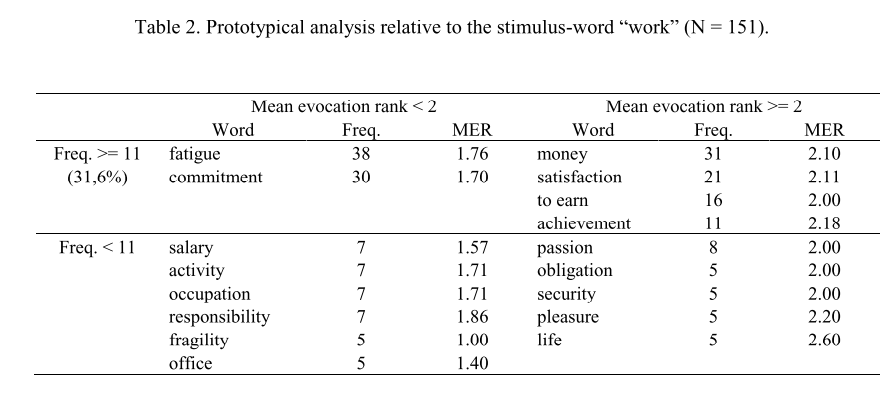
\includegraphics{images/walcheque.png}
\caption{RS de ``trabajo''}
\end{figure}

El cuadro está compuesto por 4 cuadrantes, resultante de ordenar las palabras por frecuencia y orden de evocación, ambas cortadas en 2 segmentos por el punto medio. La tabla es clara en segmentar palabras, aunque no hay manera fácil de identificar los segmentos si no es comparando frecuencias. Además, si quisierámos agregar una variable, como es valoración en nuestro caso, las tablas se vuelven extensas para compararlas.

Un gráfico debería debería permitirnos visualizar esto mejor!

Vamos a dibujar un gráfico que:
* permita dibujar puntos en el cruce de frecuencia (X) y orden de evocación (Y),
* que incluya las palabras en el gráfico, de modo tal que podamos leerlas por grupitos,
* que señale con color la valoración,
* que muestre los puntos de corte en frecuencia (X) y orden de evocación (Y),
* y que remarque el cuadrante del núcleo central.

\begin{Shaded}
\begin{Highlighting}[]
\NormalTok{prototipico }\OtherTok{\textless{}{-}} \FunctionTok{analisis\_proto}\NormalTok{(}\AttributeTok{tabla\_evocaciones =}\NormalTok{ asociaciones, }\AttributeTok{frecuencia\_minima =} \DecValTok{5}\NormalTok{, }\AttributeTok{criterio\_corte =} \StringTok{"media"}\NormalTok{)}
\end{Highlighting}
\end{Shaded}

\begin{verbatim}
## frecuencia minima = 5
\end{verbatim}

\begin{verbatim}
## valor corte frecuencia = 15.219512195122
\end{verbatim}

\begin{verbatim}
## valor corte orden = 2.87623694419952
\end{verbatim}

\begin{verbatim}
## palabras en cada segmento = 7 | 3 | 13 | 18
\end{verbatim}

\begin{Shaded}
\begin{Highlighting}[]
\FunctionTok{glimpse}\NormalTok{(prototipico)}
\end{Highlighting}
\end{Shaded}

\begin{verbatim}
## Rows: 41
## Columns: 5
## $ palabra          <chr> "información", "datos", "control", "informacion", "grande", "manipulac~
## $ freq             <int> 102, 81, 35, 28, 20, 18, 16, 34, 29, 19, 15, 10, 8, 8, 8, 7, 6, 6, 6, ~
## $ valoracion_media <dbl> 2.5784314, 2.1481481, -2.3142857, 2.2857143, 2.7000000, -3.4444444, 4.~
## $ orden_media      <dbl> 2.078431, 1.962963, 2.571429, 2.535714, 2.000000, 2.500000, 2.750000, ~
## $ segmento         <dbl> 1, 1, 1, 1, 1, 1, 1, 2, 2, 2, 3, 3, 3, 3, 3, 3, 3, 3, 3, 3, 3, 3, 3, 4~
\end{verbatim}

\begin{Shaded}
\begin{Highlighting}[]
\NormalTok{prototipico }\SpecialCharTok{\%\textgreater{}\%}
  \FunctionTok{ggplot}\NormalTok{(}\FunctionTok{aes}\NormalTok{(}\AttributeTok{x=}\NormalTok{freq,}\AttributeTok{y=}\NormalTok{orden\_media,}\AttributeTok{label=}\NormalTok{palabra)) }\SpecialCharTok{+} \CommentTok{\# frecuencia x orden}
  \FunctionTok{scale\_x\_continuous}\NormalTok{(}\AttributeTok{trans=}\StringTok{\textquotesingle{}log\textquotesingle{}}\NormalTok{) }\SpecialCharTok{+} \CommentTok{\# vamos a aplicar una transformación al eje X para ver mejor los puntos}
  \FunctionTok{geom\_hline}\NormalTok{(}\AttributeTok{yintercept =} \FloatTok{2.87623694419952}\NormalTok{, }\AttributeTok{linetype =} \DecValTok{2}\NormalTok{) }\SpecialCharTok{+} \CommentTok{\# tomamos este valor del mensaje de la función}
  \FunctionTok{geom\_vline}\NormalTok{(}\AttributeTok{xintercept =} \FloatTok{15.219512195122}\NormalTok{, }\AttributeTok{linetype =} \DecValTok{2}\NormalTok{) }\SpecialCharTok{+}  \CommentTok{\# tomamos este valor del mensaje de la función}
  \FunctionTok{geom\_point}\NormalTok{(}\FunctionTok{aes}\NormalTok{(}\AttributeTok{size=}\NormalTok{freq, }\AttributeTok{colour=}\NormalTok{valoracion\_media), }\AttributeTok{show.legend =} \ConstantTok{TRUE}\NormalTok{) }\SpecialCharTok{+} \CommentTok{\# agregamos los puntos}
  \FunctionTok{scale\_colour\_gradient}\NormalTok{(}\AttributeTok{low =} \StringTok{"red"}\NormalTok{, }\AttributeTok{high =} \StringTok{"green"}\NormalTok{, }\AttributeTok{na.value =} \ConstantTok{NA}\NormalTok{) }\SpecialCharTok{+} \CommentTok{\# gama de colores para valores continuos}
  \FunctionTok{geom\_text}\NormalTok{( }\FunctionTok{aes}\NormalTok{(}\AttributeTok{size=}\DecValTok{20}\NormalTok{, }\AttributeTok{colour=}\NormalTok{valoracion\_media), }\AttributeTok{fontface =} \StringTok{"bold"}\NormalTok{,}
             \AttributeTok{show.legend =} \ConstantTok{FALSE}\NormalTok{, }\AttributeTok{nudge\_y =} \SpecialCharTok{{-}}\NormalTok{.}\DecValTok{1}\NormalTok{, }\AttributeTok{check\_overlap =} \ConstantTok{TRUE}\NormalTok{) }\SpecialCharTok{+} \CommentTok{\# agregamos las palabras}
  \FunctionTok{labs}\NormalTok{(}\AttributeTok{y=}\StringTok{"Orden de evocación"}\NormalTok{, }\AttributeTok{x =} \StringTok{"Frecuencia (log)"}\NormalTok{) }\SpecialCharTok{+} \CommentTok{\# ponemos labels en los ejes}
  \FunctionTok{theme\_minimal}\NormalTok{() }\CommentTok{\# borremos estilos innecesarios}
\end{Highlighting}
\end{Shaded}

\includegraphics{curso-intro-r_files/figure-latex/unnamed-chunk-28-1.pdf}

\hypertarget{procesamiento-del-lenguaje-natural-y-analisis-de-sentimiento}{%
\chapter{Procesamiento del lenguaje natural y Analisis de sentimiento}\label{procesamiento-del-lenguaje-natural-y-analisis-de-sentimiento}}

En este capítulo nos introduciremos al procesamiento del lenguaje natural, y a una tarea particular de dicho campo: el análisis de sentimiento o polaridad.

Particularmente, vamos a aprender a:

\begin{enumerate}
\def\labelenumi{\arabic{enumi}.}
\tightlist
\item
  pre-procesar texto para su posterior análisis;
\item
  cruzar tablas (en nuestro caso, oraciones y diccionarios);
\item
  realizar un análisis de sentimiento, incluyendo la preparación de los datos para el uso de librerías específicas.
\end{enumerate}

Trabajaremos con un corpus de oraciones, extraídas de noticias argentinas que incluyen la palabra ``big data.'' El objetivo de nuestro análisis será \textbf{determinar si el big data es valorado como un fenómeno positivo o negativo}, de acuerdo a la carga valorativa de las palabras que le dan contexto.
Esta tarea puede ser útil para comenzar a explorar el fenómeno de la polaridad del big data. Al respecto, luego de analizar noticias acerca de big data en diarios de Estados Unidos, Reino Unido y Australia, \protect\hyperlink{ref-Paganoni2019}{Paganoni} (\protect\hyperlink{ref-Paganoni2019}{2019}) sugiere:

\begin{quote}
Big data appears to be framed between two poles---data and information as opposed to rights and privacy---whose gap has of late been emphasised by a number of data scandals affecting business, health and politics, and culminating in the major unforeseen event of Cambridge Analytica and Facebook.
\end{quote}

A lo largo de este tutorial trabajaremos con varias librerías, que podemos instalar con el siguiente código:

\begin{Shaded}
\begin{Highlighting}[]
\FunctionTok{install.packages}\NormalTok{(}\FunctionTok{c}\NormalTok{(}\StringTok{"readr"}\NormalTok{, }\StringTok{"tidyverse"}\NormalTok{, }\StringTok{"tidytext"}\NormalTok{)) }\CommentTok{\# las hemos instalado en capítulos anteriores}
\FunctionTok{install.packages}\NormalTok{(}\FunctionTok{c}\NormalTok{(}\StringTok{"udpipe"}\NormalTok{)) }\CommentTok{\# las usaremos por primera vez}
\end{Highlighting}
\end{Shaded}

\hypertarget{pre-procesamiento-de-texto}{%
\section{Pre-procesamiento de texto}\label{pre-procesamiento-de-texto}}

Naturalmente, antes de todo proyecto de análisis de datos, necesitamos datos. El dataset con el que trabajaremos en este capítulo fue construido a través de la técnica de \emph{scrapping}, que consiste en capturar datos a partir de la exploración de los elementos y anotaciones HTML de sitios webs. Ahora bien, si quisiéramos inmediatamente ``procesar'' estos datos, nos encontraríamos con varios problemas. Para empezar, ¿Cómo podríamos hacer para que el montón de textos que tenemos sea interpretable por una máquina que no habla ni entiende nuestro idioma?

Pues bien, con cualquier dataset, digamos, mayormente numérico, el problema del procesamiento consta de realizar ciertas tareas casi estandarizadas: eliminar outliers, normalizar los datos, completar o desechar valores faltantes, etc. Así, si quisiéramos analizar datos relativos a departamentos en alquiler, por ejemplo, donde nos interesaría predecir el precio de nuevas unidades en función de características como la ubicación, superficie y antigüedad, deberíamos realizar esta serie de operaciones que describimos recientemente para asegurarnos de tener los mejores resultados posibles. Esto no aplica directamente en el terreno del lenguaje natural, donde las tareas de preprocesamiento serán distintas.

El preprocesamiento de datos extraídos del lenguaje natural apunta a la construcción de una representación matemática de los mismos que, como tal, sea entendible y computable por nuestras funciones y modelos. En particular, la representación ``matemática'' de la que aquí hablaremos será la de un vector, pero hablaremos de esto un poco más adelante. Por lo pronto, es importante entender que lo que se busca es ``estructurar'' los datos ``no-estructurados'' para volverlos computables.

Para llegar a esta instancia de ``estructuración'' del lenguaje natural, el preprocesamiento deberá encargarse de una serie de operaciones sobre nuestro corpus de texto tendientes a su normalización. En este capítulo haremos 2 tareas específicas: (1) tokenización y análisis morfosintáctico, (2) reducción de las palabras del vocabulario.

Para ello empecemos por cargar los datos

\begin{Shaded}
\begin{Highlighting}[]
\FunctionTok{library}\NormalTok{(readr) }\CommentTok{\# para leer csv}
\FunctionTok{library}\NormalTok{(tidyverse) }\CommentTok{\# para manipular tablas}

\NormalTok{oraciones }\OtherTok{\textless{}{-}}\NormalTok{ readr}\SpecialCharTok{::}\FunctionTok{read\_csv}\NormalTok{(}\AttributeTok{file =} \StringTok{"https://raw.githubusercontent.com/gastonbecerra/curso{-}intro{-}r/main/data/oraciones\_entrenamiento.csv"}\NormalTok{) }\CommentTok{\# importamos datos}
\FunctionTok{glimpse}\NormalTok{(oraciones) }\CommentTok{\# miramos la estructura de la base}
\end{Highlighting}
\end{Shaded}

\begin{verbatim}
## Rows: 400
## Columns: 3
## $ doc_id  <dbl> 3578, 2300, 405, 2540, 2016, 2713, 1503, 534, 1101, 3043, 1458, 1010, 41, 2421,~
## $ oracion <chr> "vale aclarar que bigdata es el nombre que se utiliza para describir a los gran~
## $ estado  <chr> "positivo", "positivo", "positivo", "positivo", "positivo", "positivo", "positi~
\end{verbatim}

Para el análisis morfosintáctico trabajaremos con la librería UdPipe, desarrollada por el \href{https://ufal.mff.cuni.cz/udpipe}{Instituto de linguistica formal y aplicada de la Universidad de la República Checa}, que tiene un modelo para procesar texto en castellano.

Lo primero que debemos hacer es instalar la librería. Luego, deberemos descargar el modelo del idioma que nos interesa.

\begin{Shaded}
\begin{Highlighting}[]
\FunctionTok{install.packages}\NormalTok{(}\StringTok{"udpipe"}\NormalTok{) }\CommentTok{\# instalamos la libreria}
\FunctionTok{library}\NormalTok{(udpipe) }\CommentTok{\# la cargamos}
\NormalTok{modelo\_sp }\OtherTok{\textless{}{-}}\NormalTok{ udpipe}\SpecialCharTok{::}\FunctionTok{udpipe\_download\_model}\NormalTok{(}\StringTok{\textquotesingle{}spanish\textquotesingle{}}\NormalTok{) }\CommentTok{\# descarga el modelo y guarda la referencia  }
\NormalTok{modelo\_sp}\SpecialCharTok{$}\NormalTok{file\_model }\CommentTok{\# refrencia al modelo descargado}
\NormalTok{modelo\_sp }\OtherTok{\textless{}{-}} \FunctionTok{udpipe\_load\_model}\NormalTok{(}\AttributeTok{file =}\NormalTok{ modelo\_sp}\SpecialCharTok{$}\NormalTok{file\_model) }\CommentTok{\# cargamos el modelo en memoria}
\end{Highlighting}
\end{Shaded}

Con el modelo ya estamos en condiciones de empezar a \emph{parsear} nuestro corpus de oraciones, y \emph{anotar} qué tipo de componente es cada palabra.

\begin{Shaded}
\begin{Highlighting}[]
\NormalTok{oraciones\_anotadas }\OtherTok{\textless{}{-}} \FunctionTok{udpipe\_annotate}\NormalTok{( }
  \AttributeTok{object =}\NormalTok{ modelo\_sp, }\CommentTok{\# el modelo de idioma}
  \AttributeTok{x =}\NormalTok{ oraciones}\SpecialCharTok{$}\NormalTok{oracion, }\CommentTok{\# el texto a anotar, }
  \AttributeTok{doc\_id =}\NormalTok{ oraciones}\SpecialCharTok{$}\NormalTok{doc\_id, }\CommentTok{\# el id de cada oracion (el resultado tendrá 1 palabra x fila)}
  \AttributeTok{trace =} \DecValTok{100}
\NormalTok{  ) }\SpecialCharTok{\%\textgreater{}\%} \FunctionTok{as.data.frame}\NormalTok{(.) }\CommentTok{\# convertimos el resultado en data frame}
\end{Highlighting}
\end{Shaded}

Vamos a examinar la tabla con las oraciones parseadas:

\begin{Shaded}
\begin{Highlighting}[]
\FunctionTok{glimpse}\NormalTok{(oraciones\_anotadas)}
\end{Highlighting}
\end{Shaded}

\begin{verbatim}
## Rows: 12,153
## Columns: 14
## $ doc_id        <dbl> 3578, 3578, 3578, 3578, 3578, 3578, 3578, 3578, 3578, 3578, 3578, 3578, 3~
## $ paragraph_id  <dbl> 1, 1, 1, 1, 1, 1, 1, 1, 1, 1, 1, 1, 1, 1, 1, 1, 1, 1, 1, 1, 1, 1, 1, 1, 1~
## $ sentence_id   <dbl> 1, 1, 1, 1, 1, 1, 1, 1, 1, 1, 1, 1, 1, 1, 1, 1, 1, 1, 1, 1, 1, 1, 1, 1, 1~
## $ sentence      <chr> "vale aclarar que bigdata es el nombre que se utiliza para describir a lo~
## $ token_id      <chr> "1", "2", "3", "4", "5", "6", "7", "8", "9", "10", "11", "12", "13", "14"~
## $ token         <chr> "vale", "aclarar", "que", "bigdata", "es", "el", "nombre", "que", "se", "~
## $ lemma         <chr> "valer", "aclarar", "que", "bigdata", "ser", "el", "nombre", "que", "él",~
## $ upos          <chr> "VERB", "VERB", "SCONJ", "PROPN", "AUX", "DET", "NOUN", "SCONJ", "PRON", ~
## $ xpos          <lgl> NA, NA, NA, NA, NA, NA, NA, NA, NA, NA, NA, NA, NA, NA, NA, NA, NA, NA, N~
## $ feats         <chr> "Mood=Ind|Number=Sing|Person=3|Tense=Pres|VerbForm=Fin", "VerbForm=Inf", ~
## $ head_token_id <dbl> 0, 1, 7, 7, 7, 7, 2, 10, 10, 7, 12, 10, 16, 16, 16, 12, 18, 16, 21, 21, 1~
## $ dep_rel       <chr> "root", "xcomp", "mark", "nsubj", "cop", "det", "ccomp", "mark", "iobj", ~
## $ deps          <lgl> NA, NA, NA, NA, NA, NA, NA, NA, NA, NA, NA, NA, NA, NA, NA, NA, NA, NA, N~
## $ misc          <chr> NA, NA, NA, NA, NA, NA, NA, NA, NA, NA, NA, NA, NA, NA, NA, NA, NA, NA, N~
\end{verbatim}

Esta anotación se ha encargado de muchas tareas típicas del pre-procesamiento de texto:

\begin{itemize}
\tightlist
\item
  \emph{tokenización}: la unidad mínima del análisis es ahora cada palabra (notá que por eso hay muchas mas filas que antes). El \texttt{doc\_id} nos permitirá volver a unir las piezas cuando hagamos tareas por oraciones;
\item
  para cada palabra se ha anotado el tipo en \texttt{upos};
\item
  se ha convertido la palabra a su raíz en \texttt{lemma}.
\end{itemize}

Podemos usar \texttt{upos} para filtrar palabras. Este paso es una alternativa a la eliminación de \emph{stopwords} y palabras que no aportan contenido semántico de manera directa (por ejemplo, las preposiciones).

La \emph{lemmatización} es un procedimiento que busca reducir las palabras a su forma no flexionada o conjugada. Es una alternativa a la \emph{stemmization}, que intenta reducir heurística e iterativamente la extensión de las palabras, removiendo caracteres, hasta reducirlas a su raíz. Así, la expresión ``Google analiza big data para inferir el ritmo de contagio de la gripe H1N1,'' queda lemmatizada como ``google analizar bigdata inferir ritmo contagio gripe h1n1.''

\begin{Shaded}
\begin{Highlighting}[]
\NormalTok{oraciones\_anotadas2 }\OtherTok{\textless{}{-}}\NormalTok{ oraciones\_anotadas }\SpecialCharTok{\%\textgreater{}\%} 
  \FunctionTok{filter}\NormalTok{(upos}\SpecialCharTok{==}\StringTok{"ADJ"}\SpecialCharTok{|}\NormalTok{ upos}\SpecialCharTok{==}\StringTok{"VERB"}\SpecialCharTok{|}\NormalTok{ upos}\SpecialCharTok{==}\StringTok{"NOUN"} \SpecialCharTok{|}\NormalTok{ upos}\SpecialCharTok{==}\StringTok{"ADV"}\NormalTok{) }\CommentTok{\# filtramos por tipo de palabra}
\FunctionTok{glimpse}\NormalTok{(oraciones\_anotadas2)}
\end{Highlighting}
\end{Shaded}

\begin{verbatim}
## Rows: 5,445
## Columns: 14
## $ doc_id        <dbl> 3578, 3578, 3578, 3578, 3578, 3578, 3578, 3578, 3578, 3578, 3578, 3578, 3~
## $ paragraph_id  <dbl> 1, 1, 1, 1, 1, 1, 1, 1, 1, 1, 1, 1, 1, 1, 1, 1, 1, 1, 1, 1, 1, 1, 1, 1, 1~
## $ sentence_id   <dbl> 1, 1, 1, 1, 1, 1, 1, 1, 1, 1, 1, 1, 1, 1, 1, 1, 1, 1, 1, 1, 1, 1, 1, 1, 1~
## $ sentence      <chr> "vale aclarar que bigdata es el nombre que se utiliza para describir a lo~
## $ token_id      <chr> "1", "2", "7", "10", "12", "15", "16", "18", "21", "23", "25", "27", "30"~
## $ token         <chr> "vale", "aclarar", "nombre", "utiliza", "describir", "grandes", "volúmene~
## $ lemma         <chr> "valer", "aclarar", "nombre", "utilizar", "describir", "grande", "volumen~
## $ upos          <chr> "VERB", "VERB", "NOUN", "VERB", "VERB", "ADJ", "NOUN", "NOUN", "NOUN", "N~
## $ xpos          <lgl> NA, NA, NA, NA, NA, NA, NA, NA, NA, NA, NA, NA, NA, NA, NA, NA, NA, NA, N~
## $ feats         <chr> "Mood=Ind|Number=Sing|Person=3|Tense=Pres|VerbForm=Fin", "VerbForm=Inf", ~
## $ head_token_id <dbl> 0, 1, 2, 7, 10, 16, 12, 16, 16, 21, 21, 21, 21, 30, 30, 38, 35, 38, 8, 2,~
## $ dep_rel       <chr> "root", "xcomp", "ccomp", "acl:relcl", "advcl", "amod", "obl", "nmod", "a~
## $ deps          <lgl> NA, NA, NA, NA, NA, NA, NA, NA, NA, NA, NA, NA, NA, NA, NA, NA, NA, NA, N~
## $ misc          <chr> NA, NA, NA, NA, NA, NA, NA, NA, NA, NA, NA, NA, NA, NA, NA, NA, NA, NA, N~
\end{verbatim}

Es interesante señalar que pasamos de 12153 palabras parseadas y anotadas, a solo 5445, que son con las que trabajaremos.

\hypertarget{anuxe1lisis-de-sentimiento}{%
\section{Análisis de sentimiento}\label{anuxe1lisis-de-sentimiento}}

Generalmente se acepta que hay 2 métodos para este tipo de análisis:

\begin{enumerate}
\def\labelenumi{\arabic{enumi}.}
\tightlist
\item
  un enfoque basado en ``lexicos'' o ``lexicones'' (diccionarios que incluyen para cada palabra una valoración en alguna dimensión afectiva, como el agrado), y que consiste en calcular la valoración media del texto que nos interesa, a partir de pesar aquellas palabras que están en los lexicones;
\item
  un enfoque basado en clasificación / aprendizaje automático, que busca inferir reglas para establecer la polaridad de una oración a partir de estudiar un dataset de oraciones previamente clasificadas (por un humano).
\end{enumerate}

En este capítulos nos centraremos en el primer enfoque (lexicones), dejando el aprendizaje para un capítulo posterior.
Buscaremos implementar esto de dos maneras:

\begin{enumerate}
\def\labelenumi{\arabic{enumi}.}
\tightlist
\item
  en primer lugar, cruzando la tabla de oraciones con el lexicon, y haciendo nosotros alguna evaluación;
\item
  en segundo lugar, con una librería que contemple las falencias de nuestro primer enfoque.
\end{enumerate}

\hypertarget{cruce-con-lexicones}{%
\subsection{Cruce con lexicones}\label{cruce-con-lexicones}}

Ahora podemos cruzar los lemmas de nuestras oraciones con los lexicones, para calcular la orientación de cada oración que incluye big data.

Vamos a trabajar con 1 lexicón construido a partir de otros dos: 1. \emph{Spanish Dictionary Affect Language} (\texttt{sdal}), desarrollado por \protect\hyperlink{ref-Gravano2014}{Gravano and Dell'Amerlina Ríos} (\protect\hyperlink{ref-Gravano2014}{2014}), que replica el modelo de \protect\hyperlink{ref-Whissell2009}{Whissell} (\protect\hyperlink{ref-Whissell2009}{2009}). Este es un lexicon formado por 2700+ términos, clasificados manualmente en tres dimensiones afectivas, de las cuales aquí utilizamos el agrado; 2. \emph{Lexicon de evocaciones a big data} (\texttt{evoc}), desarrollado por \protect\hyperlink{ref-Becerra2020}{Becerra and López-alurralde} (\protect\hyperlink{ref-Becerra2020}{2020}) en el marco de una investigación sobre las representaciones sociales del big data con la técnica de la evocación libre de palabras, a la que se añadió la posibilidad de aclarar la valoración del término incluído. Este es un lexicon formado por 1500+ términos. Para unir estos lexicones tuvimos que lemmatizar los términos, escalar las valoraciones dentro del rango -1 y 1, eliminamos ambigüedades calculando la media.

\begin{Shaded}
\begin{Highlighting}[]
\NormalTok{lexicones }\OtherTok{\textless{}{-}}\NormalTok{ readr}\SpecialCharTok{::}\FunctionTok{read\_csv}\NormalTok{(}\StringTok{\textquotesingle{}https://raw.githubusercontent.com/gastonbecerra/curso{-}intro{-}r/main/data/lexicones.csv\textquotesingle{}}\NormalTok{)}
\end{Highlighting}
\end{Shaded}

\begin{verbatim}
## 
## -- Column specification -------------------------------------------------------------------------
## cols(
##   lemma = col_character(),
##   v = col_double()
## )
\end{verbatim}

\begin{Shaded}
\begin{Highlighting}[]
\FunctionTok{summary}\NormalTok{(lexicones)}
\end{Highlighting}
\end{Shaded}

\begin{verbatim}
##     lemma                 v          
##  Length:4005        Min.   :-1.0000  
##  Class :character   1st Qu.: 0.2000  
##  Mode  :character   Median : 0.4667  
##                     Mean   : 0.3796  
##                     3rd Qu.: 0.7333  
##                     Max.   : 1.0000
\end{verbatim}

Ahora sí: vamos a cruzar tablas! Particularmente, nos interesa ver si los lemmas que extrajimos de nuestras oraciones coinciden con los lemmas en los lexicones.
En cuyo caso, vamos a anotar la media de las valoraciones de estos lexicones, junto con la cantidad de lemmas que tomamos de cada oracion (para saber cuantos lemmas con valoraciones hay en la oracion), entre otros indicadores que podamos usar para evaluar y filtrar resultados.

Para cruzar tablas usaremos los verbos \texttt{\_join}, o más específicamente, \texttt{left\_join} que mantiene todas las filas de nuestra tabla, agregandole las columnas con los valores de otra. Para hacer el cruce de tablas, \texttt{\_join} utiliza las columnas de nombre coincidente (aunque podés especificar los pares con \texttt{by\ =\ c("x"="y")}). Esta es una opción de unión entre otras: \texttt{left\_join}, \texttt{inner\_join}, \texttt{anti\_join}.

\begin{figure}
\centering
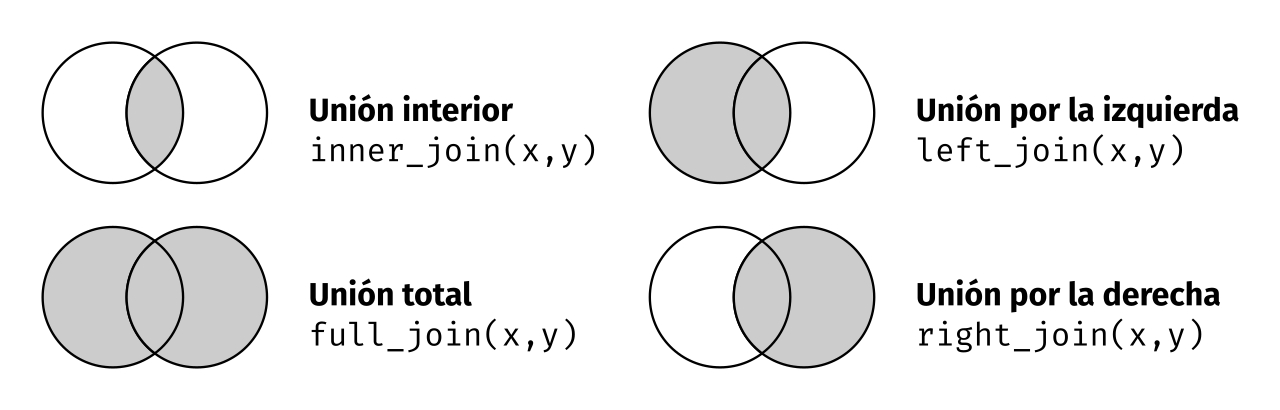
\includegraphics{images/join-venn.jpg}
\caption{Tomado de \url{https://es.r4ds.hadley.nz/datos-relacionales.html}}
\end{figure}

\begin{Shaded}
\begin{Highlighting}[]
\NormalTok{oraciones\_lexicones }\OtherTok{\textless{}{-}}\NormalTok{ oraciones\_anotadas2 }\SpecialCharTok{\%\textgreater{}\%} 
  \FunctionTok{select}\NormalTok{(doc\_id, lemma) }\SpecialCharTok{\%\textgreater{}\%} 
  \FunctionTok{mutate}\NormalTok{(}\AttributeTok{doc\_id=}\FunctionTok{as.integer}\NormalTok{(doc\_id)) }\SpecialCharTok{\%\textgreater{}\%}
  \FunctionTok{left\_join}\NormalTok{(lexicones, }\AttributeTok{by=}\StringTok{"lemma"}\NormalTok{) }\SpecialCharTok{\%\textgreater{}\%} \CommentTok{\# cruzamos con el lexicon sobre los registros de nuestra tabla}
  \FunctionTok{group\_by}\NormalTok{(doc\_id) }\SpecialCharTok{\%\textgreater{}\%} \CommentTok{\# ahora vamos a calcular valores por oración}
  \FunctionTok{summarise}\NormalTok{(}
    \AttributeTok{valor=}\FunctionTok{mean}\NormalTok{(v, }\AttributeTok{na.rm =} \ConstantTok{TRUE}\NormalTok{), }\CommentTok{\# valoración media}
    \AttributeTok{cruzadas\_n=}\FunctionTok{length}\NormalTok{(v[}\SpecialCharTok{!}\FunctionTok{is.na}\NormalTok{(v)]), }\CommentTok{\# cantidad de palabras con valoracion}
    \AttributeTok{cruzadas\_lemmas=}\FunctionTok{paste}\NormalTok{(lemma[}\SpecialCharTok{!}\FunctionTok{is.na}\NormalTok{(v)], }\AttributeTok{collapse =} \StringTok{" "}\NormalTok{) }\CommentTok{\# palabras con valoracion}
\NormalTok{  ) }

\FunctionTok{glimpse}\NormalTok{(oraciones\_lexicones)}
\end{Highlighting}
\end{Shaded}

\begin{verbatim}
## Rows: 400
## Columns: 4
## $ doc_id          <int> 10, 12, 27, 30, 32, 39, 41, 47, 52, 54, 72, 73, 74, 81, 101, 116, 117, ~
## $ valor           <dbl> 0.55729783, 0.48465926, 0.58677755, 0.42708333, 0.54875758, 0.39142857,~
## $ cruzadas_n      <int> 13, 9, 14, 8, 11, 7, 10, 7, 2, 8, 6, 15, 7, 6, 7, 4, 4, 7, 4, 8, 6, 8, ~
## $ cruzadas_lemmas <chr> "información ser utilidad estudio mercado tendencia búsqueda clase indi~
\end{verbatim}

\begin{Shaded}
\begin{Highlighting}[]
\FunctionTok{summary}\NormalTok{(oraciones\_lexicones)}
\end{Highlighting}
\end{Shaded}

\begin{verbatim}
##      doc_id         valor            cruzadas_n     cruzadas_lemmas   
##  Min.   :  10   Min.   :-0.08889   Min.   : 1.000   Length:400        
##  1st Qu.:1051   1st Qu.: 0.44121   1st Qu.: 7.000   Class :character  
##  Median :1827   Median : 0.50713   Median :10.000   Mode  :character  
##  Mean   :1869   Mean   : 0.49712   Mean   : 9.518                     
##  3rd Qu.:2778   3rd Qu.: 0.56774   3rd Qu.:12.000                     
##  Max.   :3688   Max.   : 0.86667   Max.   :21.000
\end{verbatim}

Exploremos un poco estos resultados. Busquemos oraciones con las valoraciones más altas y más bajas.
Para poder comprender mejor lo que estamos evaluando, volvamos a incluir las oraciones, previas a nuestro preprocesamiento.

\begin{Shaded}
\begin{Highlighting}[]
\NormalTok{oraciones\_lexicones }\SpecialCharTok{\%\textgreater{}\%}
  \FunctionTok{slice\_max}\NormalTok{(}\AttributeTok{order\_by =}\NormalTok{ valor, }\AttributeTok{n =} \DecValTok{10}\NormalTok{) }\SpecialCharTok{\%\textgreater{}\%}
  \FunctionTok{inner\_join}\NormalTok{(oraciones, }\AttributeTok{by=}\StringTok{"doc\_id"}\NormalTok{) }\SpecialCharTok{\%\textgreater{}\%} \CommentTok{\# indicamos el par de columnas a usar para el cruce}
  \FunctionTok{head}\NormalTok{(}\DecValTok{8}\NormalTok{)}
\end{Highlighting}
\end{Shaded}

\begin{verbatim}
## # A tibble: 8 x 6
##   doc_id valor cruzadas_n cruzadas_lemmas                oracion                           estado
##    <dbl> <dbl>      <int> <chr>                          <chr>                             <chr> 
## 1    324 0.867          4 ganador carrera caballo gracia ¿ podemos apostar al ganador en ~ posit~
## 2   2712 0.85           2 salvar vida                    mirá también ¿ puede el bigdata ~ posit~
## 3   1164 0.810          6 deporte objetivo mejorar rend~ el deporte se alía con el bigdat~ posit~
## 4   2605 0.773          2 intentar ciencia               los proponentes de bigdata tambi~ negat~
## 5   2938 0.767          2 más pequeño                    pero actualmente las usinas de b~ negat~
## 6   1114 0.757          7 nombre novedoso transformar d~ el bigdata o dataísmo , nombre d~ posit~
## 7    116 0.753          4 aplicación beneficio potencia~ ' evidentemente , las aplicacion~ posit~
## 8   1742 0.733          3 conocer bien social            es lo que se conoce como bigdata~ posit~
\end{verbatim}

\begin{Shaded}
\begin{Highlighting}[]
\NormalTok{oraciones\_lexicones }\SpecialCharTok{\%\textgreater{}\%}
  \FunctionTok{slice\_min}\NormalTok{(}\AttributeTok{order\_by =}\NormalTok{ valor, }\AttributeTok{n =} \DecValTok{10}\NormalTok{) }\SpecialCharTok{\%\textgreater{}\%}
  \FunctionTok{inner\_join}\NormalTok{(oraciones, }\AttributeTok{by=}\StringTok{"doc\_id"}\NormalTok{) }\SpecialCharTok{\%\textgreater{}\%} \CommentTok{\# indicamos el par de columnas a usar para el cruce}
  \FunctionTok{head}\NormalTok{(}\DecValTok{8}\NormalTok{)}
\end{Highlighting}
\end{Shaded}

\begin{verbatim}
## # A tibble: 8 x 6
##   doc_id   valor cruzadas_n cruzadas_lemmas                  oracion                       estado
##    <dbl>   <dbl>      <int> <chr>                            <chr>                         <chr> 
## 1    985 -0.0889          3 decir industria obligar          dijo que la industria bigdat~ negat~
## 2    129 -0.0192          4 haber gran amenaza intimidad     ' hay una gran amenaza a la ~ negat~
## 3   1064  0.0622         11 gobierno estado valley analizar~ el asesor del gobierno de es~ negat~
## 4   3367  0.0667          2 vez temer                        tal vez asuste , sí , pero n~ negat~
## 5    380  0.151           9 diferencia encuesta encuesta po~ a diferencia de una encuesta~ negat~
## 6   3412  0.170           7 empresa quedar robar informació~ tanto esta empresa como las ~ negat~
## 7   2183  0.180           9 combinación estrategia miedo mu~ la combinación de bigdata y ~ negat~
## 8   2184  0.180           9 combinación estrategia miedo mu~ la combinación de bigdata y ~ negat~
\end{verbatim}

Evaluemos los resultados y tomemos decisiones: ¿Nos resultan satisfactorios, considerando nuestros objetivos y el uso que daremos a estos datos posteriormente? ¿Queremos introducir reglas ad-hoc para mejorar estos resultados? ¿Cuántos casos se pierden por introducir reglas? ¿Cuán arbitrario se vuelve nuestro modelo?

Estamos otra vez en el momento iterativo de la exploración. Volvamos a probar introduciendo un mínimo de palabras con valoración por oración\ldots{}

\begin{Shaded}
\begin{Highlighting}[]
\NormalTok{oraciones\_lexicones }\SpecialCharTok{\%\textgreater{}\%}
  \FunctionTok{filter}\NormalTok{(cruzadas\_n}\SpecialCharTok{\textgreater{}}\DecValTok{2}\NormalTok{) }\SpecialCharTok{\%\textgreater{}\%}
  \FunctionTok{slice\_max}\NormalTok{(}\AttributeTok{order\_by =}\NormalTok{ valor, }\AttributeTok{n =} \DecValTok{10}\NormalTok{) }\SpecialCharTok{\%\textgreater{}\%}
  \FunctionTok{inner\_join}\NormalTok{(oraciones, }\AttributeTok{by=}\StringTok{"doc\_id"}\NormalTok{) }\SpecialCharTok{\%\textgreater{}\%} \CommentTok{\# indicamos el par de columnas a usar para el cruce}
  \FunctionTok{head}\NormalTok{(}\DecValTok{8}\NormalTok{)}
\end{Highlighting}
\end{Shaded}

\begin{verbatim}
## # A tibble: 8 x 6
##   doc_id valor cruzadas_n cruzadas_lemmas                oracion                           estado
##    <dbl> <dbl>      <int> <chr>                          <chr>                             <chr> 
## 1    324 0.867          4 ganador carrera caballo gracia ¿ podemos apostar al ganador en ~ posit~
## 2   1164 0.810          6 deporte objetivo mejorar rend~ el deporte se alía con el bigdat~ posit~
## 3   1114 0.757          7 nombre novedoso transformar d~ el bigdata o dataísmo , nombre d~ posit~
## 4    116 0.753          4 aplicación beneficio potencia~ ' evidentemente , las aplicacion~ posit~
## 5   1742 0.733          3 conocer bien social            es lo que se conoce como bigdata~ posit~
## 6   1133 0.722          3 herramienta transformar ciudad el bigdata va a ser una de las h~ posit~
## 7   2016 0.718          4 entender herramienta mucho bi~ hay que entender que bigdata es ~ posit~
## 8   1740 0.709          6 magia considerar clase herram~ es la magia del bigdata , consid~ posit~
\end{verbatim}

\begin{Shaded}
\begin{Highlighting}[]
\NormalTok{oraciones\_lexicones }\SpecialCharTok{\%\textgreater{}\%}
  \FunctionTok{filter}\NormalTok{(cruzadas\_n}\SpecialCharTok{\textgreater{}}\DecValTok{2}\NormalTok{) }\SpecialCharTok{\%\textgreater{}\%}
  \FunctionTok{slice\_min}\NormalTok{(}\AttributeTok{order\_by =}\NormalTok{ valor, }\AttributeTok{n =} \DecValTok{10}\NormalTok{) }\SpecialCharTok{\%\textgreater{}\%}
  \FunctionTok{inner\_join}\NormalTok{(oraciones, }\AttributeTok{by=}\StringTok{"doc\_id"}\NormalTok{) }\SpecialCharTok{\%\textgreater{}\%} \CommentTok{\# indicamos el par de columnas a usar para el cruce}
  \FunctionTok{head}\NormalTok{(}\DecValTok{8}\NormalTok{)}
\end{Highlighting}
\end{Shaded}

\begin{verbatim}
## # A tibble: 8 x 6
##   doc_id   valor cruzadas_n cruzadas_lemmas                  oracion                       estado
##    <dbl>   <dbl>      <int> <chr>                            <chr>                         <chr> 
## 1    985 -0.0889          3 decir industria obligar          dijo que la industria bigdat~ negat~
## 2    129 -0.0192          4 haber gran amenaza intimidad     ' hay una gran amenaza a la ~ negat~
## 3   1064  0.0622         11 gobierno estado valley analizar~ el asesor del gobierno de es~ negat~
## 4    380  0.151           9 diferencia encuesta encuesta po~ a diferencia de una encuesta~ negat~
## 5   3412  0.170           7 empresa quedar robar informació~ tanto esta empresa como las ~ negat~
## 6   2183  0.180           9 combinación estrategia miedo mu~ la combinación de bigdata y ~ negat~
## 7   2184  0.180           9 combinación estrategia miedo mu~ la combinación de bigdata y ~ negat~
## 8   1376  0.184           3 privacidad dato usuario          el talón de aquiles del bigd~ negat~
\end{verbatim}

Estos resultados parecen ser un poco mejores, aunque esta evaluación dependerá mucho del uso que querramos darle luego. Recordemos que el dato es un momento en un proceso\ldots{}

Ahora que podemos intuir los límites y potenciales de este tipo de procesamiento del lenguaje, vamos a volver a realizar estos análisis, con un procedimiento mucho más robusto, utilizando funciones de librerías o packages.

\hypertarget{uso-de-packages}{%
\subsection{Uso de packages}\label{uso-de-packages}}

En lo que sigue vamos a realizar \emph{sentiment analysis} utilizando packages, particularmente con \texttt{txt\_sentiment} del package \texttt{Udpipe} que ya usamos para anotar las oraciones.

Los pasos generales cuando quieras trabajar con funciones de packages son:

\begin{enumerate}
\def\labelenumi{\arabic{enumi}.}
\tightlist
\item
  consultar la documentación;
\item
  preprocesar los datos y transformar los objetos;
\item
  usar la función y evaluar los resultados;
\end{enumerate}

Primero, vamos a consultar la documentación del package para conocer qué funciones podemos ejecturar.
Un buen punto de entrada es consultar la vignette, generalmente una suerte de introducción rápida del pack.

\begin{Shaded}
\begin{Highlighting}[]
\FunctionTok{browseVignettes}\NormalTok{(}\StringTok{"udpipe"}\NormalTok{)}
\end{Highlighting}
\end{Shaded}

Otra opción es ir directamente a la documentación de la función, en la que encontraremos una descripción de los parámetros y ejemplos:

\begin{Shaded}
\begin{Highlighting}[]
\NormalTok{?udpipe}\SpecialCharTok{::}\NormalTok{txt\_sentiment}
\end{Highlighting}
\end{Shaded}

Veamos qué debemos especificar en esta función:

\begin{itemize}
\tightlist
\item
  \texttt{x} es el dataframe que devuelve el preprocesamiento con udpipe;
\item
  \texttt{term} es el nombre de la columna (dentro de \texttt{x}) que contiene las oraciones a analizar;
\item
  \texttt{polarity\_terms} es un dataframe que contiene 2 columnas: términos (\texttt{terms}) y polaridad (\texttt{polarity}), que puede ser de 1 o -1.
\item
  \texttt{polarity\_negators} , \texttt{polarity\_amplifiers}, \texttt{polarity\_deamplifiers} son vectores de palabras que niegan, aumentan o reducen la orientación de las palabras (por ejemplo, si tenemos ``bueno'' en el lexicon con una valoración de 1, y ``muy'' dentro de los amplifiers, ``muy bueno'' podría suponer una valoración más alta que la dada por el lexicon, con un factor que se explicita en \texttt{amplifier\_weight}). La ventana de palabras en las que se buscan estas palabras se configura con \texttt{n\_before} y \texttt{n\_after}.
\end{itemize}

Vamos a preparar los datos para cumplir estos parámetros:

\begin{Shaded}
\begin{Highlighting}[]
\CommentTok{\# preparamos el lexicon para que los términos tengan 2 valores: 1 positivas y {-}1 negativas}
\NormalTok{polarity\_terms }\OtherTok{\textless{}{-}}\NormalTok{ lexicones }\SpecialCharTok{\%\textgreater{}\%}
  \FunctionTok{mutate}\NormalTok{(}\AttributeTok{polarity =} \FunctionTok{if\_else}\NormalTok{(v}\SpecialCharTok{\textgreater{}}\DecValTok{0}\NormalTok{,}\DecValTok{1}\NormalTok{,}\SpecialCharTok{{-}}\DecValTok{1}\NormalTok{)) }\SpecialCharTok{\%\textgreater{}\%}
  \FunctionTok{select}\NormalTok{(}\AttributeTok{term=}\NormalTok{lemma, polarity)}

\CommentTok{\# preparamos los términos que modifican pesos}
\NormalTok{polarity\_negators }\OtherTok{\textless{}{-}} \FunctionTok{c}\NormalTok{(}\StringTok{"no"}\NormalTok{,}\StringTok{"nunca"}\NormalTok{,}\StringTok{"nadie"}\NormalTok{)}
\NormalTok{polarity\_amplifiers }\OtherTok{\textless{}{-}} \FunctionTok{c}\NormalTok{(}\StringTok{"muy"}\NormalTok{, }\StringTok{"mucho"}\NormalTok{, }\StringTok{"mas"}\NormalTok{)}
\NormalTok{polarity\_deamplifiers }\OtherTok{\textless{}{-}} \FunctionTok{c}\NormalTok{(}\StringTok{"poco"}\NormalTok{, }\StringTok{"casi"}\NormalTok{, }\StringTok{"alguno"}\NormalTok{, }\StringTok{"menos"}\NormalTok{)}
\end{Highlighting}
\end{Shaded}

Recordemos que tenemos las oraciones ya preprocesadas con \texttt{udpipe} en \texttt{oraciones\_anotadas2}.

Todo listo! Corremos la función y vemos el objeto resultante.

\begin{Shaded}
\begin{Highlighting}[]
\NormalTok{oraciones\_txt\_sentiment }\OtherTok{\textless{}{-}} \FunctionTok{txt\_sentiment}\NormalTok{(}
  \AttributeTok{x =}\NormalTok{ oraciones\_anotadas2,}
  \AttributeTok{term =} \StringTok{"lemma"}\NormalTok{,}
  \AttributeTok{polarity\_terms =}\NormalTok{ polarity\_terms,}
  \AttributeTok{polarity\_negators =}\NormalTok{ polarity\_negators,}
  \AttributeTok{polarity\_amplifiers =}\NormalTok{ polarity\_amplifiers,}
  \AttributeTok{polarity\_deamplifiers =}\NormalTok{ polarity\_deamplifiers)}

\FunctionTok{glimpse}\NormalTok{(oraciones\_txt\_sentiment)}
\end{Highlighting}
\end{Shaded}

\begin{verbatim}
## List of 2
##  $ data   :'data.frame': 5445 obs. of  16 variables:
##   ..$ doc_id            : num [1:5445] 3578 3578 3578 3578 3578 ...
##   ..$ paragraph_id      : num [1:5445] 1 1 1 1 1 1 1 1 1 1 ...
##   ..$ sentence_id       : num [1:5445] 1 1 1 1 1 1 1 1 1 1 ...
##   ..$ sentence          : chr [1:5445] "vale aclarar que bigdata es el nombre que se utiliza para describir a los grandes volúmenes de información , su"| __truncated__ "vale aclarar que bigdata es el nombre que se utiliza para describir a los grandes volúmenes de información , su"| __truncated__ "vale aclarar que bigdata es el nombre que se utiliza para describir a los grandes volúmenes de información , su"| __truncated__ "vale aclarar que bigdata es el nombre que se utiliza para describir a los grandes volúmenes de información , su"| __truncated__ ...
##   ..$ token_id          : chr [1:5445] "1" "2" "7" "10" ...
##   ..$ token             : chr [1:5445] "vale" "aclarar" "nombre" "utiliza" ...
##   ..$ lemma             : chr [1:5445] "valer" "aclarar" "nombre" "utilizar" ...
##   ..$ upos              : chr [1:5445] "VERB" "VERB" "NOUN" "VERB" ...
##   ..$ xpos              : logi [1:5445] NA NA NA NA NA NA ...
##   ..$ feats             : chr [1:5445] "Mood=Ind|Number=Sing|Person=3|Tense=Pres|VerbForm=Fin" "VerbForm=Inf" "Gender=Masc|Number=Sing" "Mood=Ind|Number=Sing|Person=3|Tense=Pres|VerbForm=Fin" ...
##   ..$ head_token_id     : num [1:5445] 0 1 2 7 10 16 12 16 16 21 ...
##   ..$ dep_rel           : chr [1:5445] "root" "xcomp" "ccomp" "acl:relcl" ...
##   ..$ deps              : logi [1:5445] NA NA NA NA NA NA ...
##   ..$ misc              : chr [1:5445] NA NA NA NA ...
##   ..$ polarity          : num [1:5445] 1 NA 1 1 1 1 1 1 1 1 ...
##   ..$ sentiment_polarity: num [1:5445] 1 NA 1 1 1 1 1 1 1 1 ...
##   ..- attr(*, "spec")=
##   .. .. cols(
##   .. ..   doc_id = col_double(),
##   .. ..   paragraph_id = col_double(),
##   .. ..   sentence_id = col_double(),
##   .. ..   sentence = col_character(),
##   .. ..   token_id = col_character(),
##   .. ..   token = col_character(),
##   .. ..   lemma = col_character(),
##   .. ..   upos = col_character(),
##   .. ..   xpos = col_logical(),
##   .. ..   feats = col_character(),
##   .. ..   head_token_id = col_double(),
##   .. ..   dep_rel = col_character(),
##   .. ..   deps = col_logical(),
##   .. ..   misc = col_character()
##   .. .. )
##  $ overall:Classes 'data.table' and 'data.frame':    400 obs. of  8 variables:
##   ..$ doc_id             : num [1:400] 3578 2300 405 2540 2016 ...
##   ..$ sentiment_polarity : num [1:400] 12 15 10 7 4 9 7 10 6 13 ...
##   ..$ sentences          : int [1:400] 1 1 1 1 1 1 1 1 1 1 ...
##   ..$ terms              : int [1:400] 18 18 12 9 6 17 9 14 8 15 ...
##   ..$ terms_positive     : chr [1:400] "almacenamiento, análisis, clasificación, describir, grande, información, múltiple, nombre, surgir, través, util"| __truncated__ "ayudar, cosa, decisión, empresa, escala, generar, gran, información, internet, mejor, pensar, permitir, proyect"| __truncated__ "categoría, crear, disponer, empresa, entorno, grande, hacer, partir, tecnología, virtual" "beneficio, conseguir, fútbol, mucho, real, realmente, ventaja" ...
##   ..$ terms_negative     : chr [1:400] "dispositivo" "" "" "" ...
##   ..$ terms_negation     : chr [1:400] "" "" "" "" ...
##   ..$ terms_amplification: chr [1:400] "" "" "" "" ...
##   ..- attr(*, ".internal.selfref")=<externalptr>
\end{verbatim}

Este tipo de objetos son muy comunes en los objetos que devuelven las funciones y modelos. Se trata de una lista: un objeto que aloja otros objetos, como por ejemplo, un dataframe y un vector. Accedemos a estos elementos con el operador \texttt{\$}.

En el caso del objeto devuelto por \texttt{txt\_sentiment}, hay 2 objetos que podemos consultar

\begin{itemize}
\tightlist
\item
  \texttt{oraciones\_txt\_sentiment\$data} que tiene la tabla resultante del cruce de las oraciones anotadas (recordemos: 1 fila x lemma) con los diccionarios y modificadores, dando un valor final \texttt{oraciones\_txt\_sentiment\$data\$sentiment\_polarity};
\item
  \texttt{oraciones\_txt\_sentiment\$overall} que tiene la tabla con los valores a nivel oración, incluyendo la polaridad en \texttt{oraciones\_txt\_sentiment\$overall\$sentiment\_polarity};
\end{itemize}

Veamos este último objeto, para evaluar los resultados:

\begin{Shaded}
\begin{Highlighting}[]
\NormalTok{oraciones\_txt\_sentiment}\SpecialCharTok{$}\NormalTok{overall }\SpecialCharTok{\%\textgreater{}\%} 
  \FunctionTok{slice\_max}\NormalTok{(}\AttributeTok{order\_by =}\NormalTok{ sentiment\_polarity, }\AttributeTok{n=}\DecValTok{10}\NormalTok{) }\SpecialCharTok{\%\textgreater{}\%}
  \FunctionTok{left\_join}\NormalTok{(oraciones, }\AttributeTok{by=}\StringTok{"doc\_id"}\NormalTok{)}
\end{Highlighting}
\end{Shaded}

\begin{verbatim}
##     doc_id sentiment_polarity sentences terms
##  1:   3644                 21         1    21
##  2:   3643                 21         1    22
##  3:   3521                 17         1    20
##  4:   3567                 17         1    21
##  5:   1380                 16         1    21
##  6:   2772                 16         1    19
##  7:    866                 16         1    21
##  8:   2300                 15         1    18
##  9:   2774                 15         1    21
## 10:   3439                 15         1    19
## 11:   1395                 15         1    21
## 12:    817                 15         1    17
## 13:   2022                 15         1    21
## 14:     73                 15         1    20
## 15:   3157                 15         1    17
## 16:   2499                 15         1    18
## 17:   1038                 15         1    21
## 18:   3166                 15         1    21
## 19:    492                 15         1    21
## 20:    172                 15         1    22
##                                                                                                                                                                                           terms_positive
##  1: algoritmo, alimentar, cerebro, conformar, constituir, controlar, dato, digital, diverso, economía, especie, inteligencia_artificial, más, masa, materia, nuevo, permitir, primo, sector, ser, social
##  2: algoritmo, alimentar, cerebro, conformar, constituir, controlar, dato, digital, diverso, economía, especie, inteligencia_artificial, más, masa, materia, nuevo, permitir, primo, sector, ser, social
##  3:                                                  caso, combinación, dar, demostrar, diferente, estudio, hardware, mejor, mercado, reciente, requerir, resultado, servicio, software, tecnología, uso
##  4:                                        adquirir, alto, cliente, conservar, desarrollar, fuente, identificar, impacto, ingreso, más, nuevo, opción, principalmente, producto, servicio, utilizar, vez
##  5:                                           almacenamiento, análisis, comportamiento, dato, diverso, fin, grande, información, masivo, referir, registro, sistema, social, tendencia, término, volumen
##  6:                                                                        decisión, día, estar, libre, más, mercado, millón, país, permitir, procesar, publicación, tecnología, tomar, utilizar, vender
##  7:                                          análisis, ayudar, conocimiento, convertir, cotidiano, datar, dato, encontrar, flujo, futuro, grande, herramienta, información, partir, solución, tecnología
##  8:                                                                   ayudar, cosa, decisión, empresa, escala, generar, gran, información, internet, mejor, pensar, permitir, proyecto, tendencia, tomar
##  9:                                                                     adquirir, análisis, área, científico, concepto, dato, decisión, enorme, estrategia, importancia, nota, potencial, técnico, tener
## 10:                                                                    acuerdo, anunciar, aplicación, caso, cliente, dato, desarrollar, desear, empresa, interno, lanzar, paquete, producto, uso, vender
## 11:                                          asistencia, atención, científico, conocimiento, dato, experiencia, grande, mejor, objetivo, paciente, profesional, proporcionar, salud, tener, uso, volumen
## 12:                                                                     alcanzar, analizar, crear, dato, establecer, fenómeno, leer, millón, patrón, poder, posibilidad, real, solución, tiempo, valioso
## 13:                                                               análisis, analizar, cantidad, complejo, comprar, factor, haber, información, inmenso, llegar, patrón, persona, producto, simple, subir
## 14:                                                                                 acceso, adaptar, aprovechar, dato, decisión, empresa, forma, más, proceso, producir, rápido, saber, tema, tomar, uso
## 15:                                                                 analizar, cantidad, capacidad, capturar, dato, decisión, enorme, generación, herramienta, llamar, real, tener, tiempo, tomar, último
## 16:                                                                calidad, eficacia, establecimiento, hacer, herramienta, impacto, incorporar, información, lograr, mayor, modelo, modo, posible, tener
## 17:                                                      aplicación, cantidad, dato, enorme, grande, información, interminable, procesamiento, real, tendencia, tiempo, traer, transmitir, útil, volumen
## 18:                                                    capturar, considerar, definición, gestionar, habilidad, hacer, herramienta, información, período, procesar, referencia, siguiente, tamaño, tiempo
## 19:                                                     analizar, concepto, costumbre, crecer, diseñar, fuerte, gente, información, mejor, mucho, obtener, sector, señalar, sistema, transportar, viajar
## 20:                                                    analizar, celular, costo, dato, decir, desarrollar, desarrollo, director, encargado, fuente, herramienta, llevar, lograr, mucho, tecnología, usar
##     terms_negative terms_negation terms_amplification
##  1:                                                  
##  2:                                                  
##  3:                                                  
##  4:        negocio                                   
##  5:                                                  
##  6:                                                  
##  7:       problema                                   
##  8:                                                  
##  9:                                                  
## 10:                                                  
## 11:       personal                                   
## 12:                                                  
## 13:                                                  
## 14:                                                  
## 15:                                                  
## 16:                                                  
## 17:                                                  
## 18:                                                  
## 19:     transporte                                   
## 20:        negocio                                   
##                                                                                                                                                                                                                                                                          oracion
##  1:       y es que los datos en masa ( o ' bigdata<U+0094> ) constituyen la materia prima de la nueva economía digital : alimentan los algoritmos y la inteligencia_artificial , conformando una especie de ' cerebro social ' que permite controlar los más diversos sectores .
##  2:               y es que los datos en masa ( ' bigdata ' ) constituyen la materia prima de la nueva economía digital : alimentan los algoritmos y la inteligencia_artificial , conformando una especie de ' cerebro social ' que permite controlar los más diversos sectores .
##  3:                 un reciente estudio de idc ( international data corporation ) sobre usos y mercados para la tecnología y servicios de bigdata demuestra que cada caso requiere combinaciones diferentes de software , hardware y servicios para dar los mejores resultados .
##  4:           utilizado principalmente para identificar nuevas fuentes de ingresos ( 94% ) , conservar y adquirir clientes ( 90% ) y desarrollar nuevos productos y servicios ( 89% ) , el bigdata se posiciona cada vez más como una opción de alto impacto para los negocios .
##  5:     el término ' bigdata ' - o datos masivos - , refiere al registro , almacenamiento y análisis de grandes volúmenes de información recolectados por sistemas informáticos para diversos fines , desde publicitarios a detección de comportamientos o tendencias sociales .
##  6:                                                   nosotros le proveemos y utilizamos tecnología de bigdata y todos los días procesamos más de 40 millones de publicaciones de mercado libre en los 17 países donde está , para tomar decisiones que les permita vender más .
##  7:                 convertir datos en conocimiento bigdata , data mining e internet_cosas son las herramientas y tecnologías que ayudarán –en un futuro cercano– a encontrar soluciones a problemas cotidianos a partir del análisis de grandes flujos de datos e información .
##  8:                                         la internet de las cosas es una tendencia que se complementa con bigdata y puede ayudar a generar información que permita a las empresas tomar mejores decisiones : ' vamos a poder pensar en proyectos de gran escala ' , subrayó .
##  9: nota relacionada : ' bigdata es un concepto que tiene un potencial enorme ' estas técnicas han adquirido enorme importancia en áreas tales como estrategias de mercadeo , soporte de decisiones , planeamiento financiero y el análisis de datos científicos , entre otras .
## 10:                                                         telefónica y huawei anunciaron un acuerdo para lanzar un paquete de productos de bigdata orientados a empresas que desean desarrollar tanto casos de uso internos como vender aplicaciones de datos a sus clientes .
## 11: el uso de grandes volúmenes de datos o bigdata en la asistencia sanitaria ' tiene como objetivo proporcionar a cada paciente una atención personalizada , que combine los mejores conocimientos científicos con la experiencia personal de los profesionales de la salud ' .
## 12:                                                                                    con el fenómeno de bigdata se crearon soluciones tecnológicas que alcanzan su poder : la posibilidad de leer millones de datos en tiempo real , analizar y establecer patrones valiosos .
## 13:                  hay simples ( subir varios escalones para llegar a la terraza ) y complejos ( los factores que una persona analiza para comprar un producto ) bigdata : análisis y cruzamiento de una inmensa cantidad de información para detectar patrones determinados .
## 14:                                                                          ' el uso de bigdata produce un acceso más rápido y certero ; el tema es saber cómo las empresas van a aprovechar esos datos para tomar decisiones en forma ágil y adaptar sus procesos velozmente .
## 15:                                                                             se llama ' bigdata ' , y es una herramienta tecnológica de última generación , que tiene la capacidad de capturar y analizar una enorme cantidad de datos en tiempo real para tomar decisiones .
## 16:                                                   lo hacen mediante herramientas de bigdata , modelos scoring e incorporando información de calidad para tener mayor eficacia en la detección cuando van a un establecimiento , de modo de lograr el mayor impacto posible .
## 17:      el abanico de aplicaciones es interminable ; toda información que pueda ser útil en tiempo real puede ser transmitida y procesada , aún en enormes volúmenes , lo que trae aparejada otra tendencia llamada bigdata para procesamiento de grandes cantidades de datos .
## 18:           se puede considerar la siguiente definición : bigdata hace referencia a la información cuyo tamaño excede la habilidad de las herramientas utilizadas actualmente para capturar , gestionar y procesar la información , dentro de un período de tiempo aceptable .
## 19:                                  agosta señaló que ' está creciendo en el sector transporte muy fuerte el concepto de bigdata : analizar cómo viaja la gente , obtener esa información , sus costumbres y preferencias , para poder diseñar un mejor sistema de transporte .
## 20:                               ' logramos desarrollar una tecnología asertiva usando como fuente bigdata y herramientas de muy bajo costo para analizar los datos y llevar al celular de cada encargado ' , dice rafael sánchez , director de desarrollo de negocios de bsg .
##       estado
##  1: positivo
##  2: positivo
##  3: positivo
##  4: positivo
##  5: positivo
##  6: positivo
##  7: positivo
##  8: positivo
##  9: positivo
## 10: positivo
## 11: positivo
## 12: positivo
## 13: positivo
## 14: positivo
## 15: positivo
## 16: positivo
## 17: positivo
## 18: positivo
## 19: positivo
## 20: positivo
\end{verbatim}

\begin{Shaded}
\begin{Highlighting}[]
\NormalTok{oraciones\_txt\_sentiment}\SpecialCharTok{$}\NormalTok{overall }\SpecialCharTok{\%\textgreater{}\%} 
  \FunctionTok{slice\_min}\NormalTok{(}\AttributeTok{order\_by =}\NormalTok{ sentiment\_polarity, }\AttributeTok{n=}\DecValTok{10}\NormalTok{) }\SpecialCharTok{\%\textgreater{}\%}
  \FunctionTok{left\_join}\NormalTok{(oraciones, }\AttributeTok{by=}\StringTok{"doc\_id"}\NormalTok{)}
\end{Highlighting}
\end{Shaded}

\begin{verbatim}
##     doc_id sentiment_polarity sentences terms
##  1:   1717                 -5         1    16
##  2:   3566                 -2         1     9
##  3:   2206                 -2         1    10
##  4:    348                 -2         1    15
##  5:   3680                 -2         1     7
##  6:     12                 -1         1    12
##  7:   2770                 -1         1    14
##  8:   1952                 -1         1    13
##  9:    123                 -1         1    10
## 10:    985                 -1         1     5
## 11:   1412                 -1         1    15
##                                                                                  terms_positive
##  1:          área, común, dato, dirección, disponible, empresa, organización, percibir, sistema
##  2:                                                           dar, nube, rápido, solución, usar
##  3:                                                           democracia, institución, preparar
##  4:                                             dar, decir, marco, peña, querer, tiempo, último
##  5:                                                                            mucho, necesitar
##  6:                 acostumbrar, conocer, generación, hacer, información, joven, querer, último
##  7:                                                            aparecer, profesión, programador
##  8: altura, ciudad, comunicación, demanda, estar, generar, principal, procesamiento, territorio
##  9:                      almacenamiento, analizar, apuntar, ejecutivo, hacer, información, solo
## 10:                                                                                       decir
## 11:        claramente, confesar, defensa, encontrar, fila, lado, mismo, oscuro, sistema, virtud
##         terms_negative terms_negation terms_amplification
##  1:                                no                    
##  2:               caro             no                    
##  3:           destruir             no                    
##  4:        dispositivo             no                    
##  5:                                no                    
##  6:                                no                    
##  7:                                no                    
##  8:                                no                    
##  9:                                no                    
## 10: industria, obligar                                   
## 11:            víctima             no                    
##                                                                                                                                                                                                        oracion
##  1:                     es común detectar ' silos ' de datos , en sistemas erp o crm no disponibles a toda la organización ; o empresas cuyas direcciones aún no perciben a bigdata como un área estratégica .
##  2:                                                                                                                            usar bigdata ' no es caro , porque la nube te da soluciones rápidas y baratas .
##  3:                           la democracia representativa no está preparada para el bigdata y está siendo destruida ¿ y la democracia es una de esas instituciones que está siendo destruida por el bigdata ?
##  4:                               <U+0096> ¿ quieren decir que no fueron seducidos por la sobredimensión que se le dio en el último tiempo al dispositivo comunicacional durán barba - marcos peña - bigdata ?
##  5:                                                                                                                             ya es así y no necesitamos el bigdata porque estamos muy acostumbrados a eso .
##  6:                       ' ahora todo lo que se hace se conoce , todo es ' bigdata ' y uno no quiere que esa información se conozca ; pero los jóvenes , la última generación , se está acostumbrando a eso .
##  7:                            nos rayan los ' cerebritos ' no busques nada a lo black mirror en el ranking , pues no aparecen profesiones relacionadas con el bigdata ni tampoco programadores informáticos .
##  8: fuera de las cuatro o cinco ciudades principales , las comunicaciones en el ochenta por ciento del territorio son pésimas y no están a la altura de la demanda que genera el procesamiento de la bigdata .
##  9:                                                               ' hasta que no se pueda analizar la información , lo que se estará haciendo no es bigdata , es solo almacenamiento ' , apuntó el ejecutivo .
## 10:                                                                                                                                                  dijo que la industria bigdata obliga a la modernización .
## 11:                 ella misma confiesa que no se encuentra entre las filas de los predicadores de las virtudes del bigdata y se alinea claramente en la defensa de las víctimas del lado oscuro del sistema .
##       estado
##  1: negativo
##  2: positivo
##  3: negativo
##  4: negativo
##  5: negativo
##  6: negativo
##  7: negativo
##  8: negativo
##  9: negativo
## 10: negativo
## 11: negativo
\end{verbatim}

\texttt{txt\_sentiment} suma los scores de las palabras por oración, lo que hace esperable que las oraciones más largas muestren una polaridad más extrema. Por ello tal vez convenga normalizar este score por la cantidad de palabras en cada oración:

\begin{Shaded}
\begin{Highlighting}[]
\NormalTok{oraciones\_txt\_sentiment}\SpecialCharTok{$}\NormalTok{overall }\SpecialCharTok{\%\textgreater{}\%} 
  \FunctionTok{mutate}\NormalTok{(}\AttributeTok{sentiment\_polarity2=}\NormalTok{sentiment\_polarity}\SpecialCharTok{/}\NormalTok{terms) }\SpecialCharTok{\%\textgreater{}\%}
  \FunctionTok{slice\_max}\NormalTok{(}\AttributeTok{order\_by =}\NormalTok{ sentiment\_polarity2, }\AttributeTok{n=}\DecValTok{10}\NormalTok{) }\SpecialCharTok{\%\textgreater{}\%}
  \FunctionTok{left\_join}\NormalTok{(oraciones, }\AttributeTok{by=}\StringTok{"doc\_id"}\NormalTok{) }\SpecialCharTok{\%\textgreater{}\%}
  \FunctionTok{select}\NormalTok{(sentiment\_polarity2,oracion)}
\end{Highlighting}
\end{Shaded}

\begin{verbatim}
##     sentiment_polarity2
##  1:           1.0000000
##  2:           0.9545455
##  3:           0.9333333
##  4:           0.9285714
##  5:           0.9166667
##  6:           0.9166667
##  7:           0.9090909
##  8:           0.9000000
##  9:           0.8888889
## 10:           0.8888889
##                                                                                                                                                                                                                                                                    oracion
##  1: y es que los datos en masa ( o ' bigdata<U+0094> ) constituyen la materia prima de la nueva economía digital : alimentan los algoritmos y la inteligencia_artificial , conformando una especie de ' cerebro social ' que permite controlar los más diversos sectores .
##  2:         y es que los datos en masa ( ' bigdata ' ) constituyen la materia prima de la nueva economía digital : alimentan los algoritmos y la inteligencia_artificial , conformando una especie de ' cerebro social ' que permite controlar los más diversos sectores .
##  3:                                                                            con los nuevos cambios la empresa quiere poner al usuario en el centro de la compañía a través seis elementos claves entre los que destacan el ' bigdata ' y la ' internet de las cosas ' .
##  4:                                                                          como resultado de este trabajo y mediante el uso de herramientas de análisis de bigdata , se lograron desarrollar algoritmos que nos permiten proyectar rendimientos para la futura campaña .
##  5:                                                                                        rojas planteó que este año , el crecimiento del mercado de bigdata será de entre 26 y 30% , lo que representa un nivel de crecimiento mucho mayor que el de otras tecnologías .
##  6:                                                                                                                            ' cuando hablamos de bigdata , el principal uso que hacemos es construir productos que la gente quiere para generar comunidad ' , aseguró .
##  7:                                                                                                                                                         el bigdata aporta mucho al deporte más popular del mundo a la hora de generar , enviar y recibir información .
##  8:                                                                                                                                            el análisis de bigdata ayuda a las organizaciones a aprovechar sus datos y utilizar para identificar nuevas oportunidades .
##  9:                                                                                                                                                  para las empresas con gran cantidad de procesos operativos , bigdata puede ofrecer frutos inmediatos o quick - wins .
## 10:                                                                                                                                      ' la bigdata que genera un sitio como vorterix ayuda en parte a ver cuáles son los comportamientos de los usuarios de ese sitio .
\end{verbatim}

\begin{Shaded}
\begin{Highlighting}[]
\NormalTok{oraciones\_txt\_sentiment}\SpecialCharTok{$}\NormalTok{overall }\SpecialCharTok{\%\textgreater{}\%} 
  \FunctionTok{mutate}\NormalTok{(}\AttributeTok{sentiment\_polarity2=}\NormalTok{sentiment\_polarity}\SpecialCharTok{/}\NormalTok{terms) }\SpecialCharTok{\%\textgreater{}\%}
  \FunctionTok{slice\_min}\NormalTok{(}\AttributeTok{order\_by =}\NormalTok{ sentiment\_polarity2, }\AttributeTok{n=}\DecValTok{10}\NormalTok{) }\SpecialCharTok{\%\textgreater{}\%}
  \FunctionTok{left\_join}\NormalTok{(oraciones, }\AttributeTok{by=}\StringTok{"doc\_id"}\NormalTok{) }\SpecialCharTok{\%\textgreater{}\%}
  \FunctionTok{select}\NormalTok{(sentiment\_polarity2,oracion)}
\end{Highlighting}
\end{Shaded}

\begin{verbatim}
##     sentiment_polarity2
##  1:         -0.31250000
##  2:         -0.28571429
##  3:         -0.22222222
##  4:         -0.20000000
##  5:         -0.20000000
##  6:         -0.13333333
##  7:         -0.10000000
##  8:         -0.08333333
##  9:         -0.07692308
## 10:         -0.07142857
##                                                                                                                                                                                                        oracion
##  1:                     es común detectar ' silos ' de datos , en sistemas erp o crm no disponibles a toda la organización ; o empresas cuyas direcciones aún no perciben a bigdata como un área estratégica .
##  2:                                                                                                                             ya es así y no necesitamos el bigdata porque estamos muy acostumbrados a eso .
##  3:                                                                                                                            usar bigdata ' no es caro , porque la nube te da soluciones rápidas y baratas .
##  4:                           la democracia representativa no está preparada para el bigdata y está siendo destruida ¿ y la democracia es una de esas instituciones que está siendo destruida por el bigdata ?
##  5:                                                                                                                                                  dijo que la industria bigdata obliga a la modernización .
##  6:                               <U+0096> ¿ quieren decir que no fueron seducidos por la sobredimensión que se le dio en el último tiempo al dispositivo comunicacional durán barba - marcos peña - bigdata ?
##  7:                                                               ' hasta que no se pueda analizar la información , lo que se estará haciendo no es bigdata , es solo almacenamiento ' , apuntó el ejecutivo .
##  8:                       ' ahora todo lo que se hace se conoce , todo es ' bigdata ' y uno no quiere que esa información se conozca ; pero los jóvenes , la última generación , se está acostumbrando a eso .
##  9: fuera de las cuatro o cinco ciudades principales , las comunicaciones en el ochenta por ciento del territorio son pésimas y no están a la altura de la demanda que genera el procesamiento de la bigdata .
## 10:                            nos rayan los ' cerebritos ' no busques nada a lo black mirror en el ranking , pues no aparecen profesiones relacionadas con el bigdata ni tampoco programadores informáticos .
\end{verbatim}

Tiene bastante sentido, no?

\hypertarget{modelado-de-topicos}{%
\chapter{Modelado de topicos}\label{modelado-de-topicos}}

En este capítulo nos introduciremos a una técnica de aprendizaje no supervisado en el campo del procesamiento del lenguaje natural: el modelado de tópicos (\emph{topic modeling}). Esta técnica busca construir tópicos o temas en base a las distribuciones de palabras en un conjunto de documentos.

A lo largo de este ejercicio veremos:

\begin{enumerate}
\def\labelenumi{\arabic{enumi}.}
\tightlist
\item
  cómo pre-procesar texto para su posterior análisis;
\item
  cómo construir vectores de documentos por términos;
\item
  cómo modelar tópicos;
\item
  cómo interpretar los tópicos, leyendo los resultados junto con nuestro propio análisis cualitativo, entre otras indagaciones.
\end{enumerate}

Vamos a utilizar esta técnica para intentar explorar \textbf{¿Cuál es la tematización del big data en la prensa?}, utilizando un corpus de noticias que incluyen la palabra ``big data,'' tomadas de periódicos digitales argentinos. Nos interesa particularmente indagar de qué manera el big data es contextualizado, de modo tal que el modelado de tópicos pueden asistir al análisis de ``frames'' discursivos. Este tipo de análisis son útiles para investigar acerca de la construcción social de un fenómeno por parte de un sistema de comunicación, como es la prensa (\protect\hyperlink{ref-Jacobi2016}{Jacobi, Atteveldt, and Welbers 2016}).

A lo largo de este tutorial trabajaremos con varias librerías, que podemos instalar con el siguiente código:

\begin{Shaded}
\begin{Highlighting}[]
\FunctionTok{install.packages}\NormalTok{(}\FunctionTok{c}\NormalTok{(}\StringTok{"readr"}\NormalTok{, }\StringTok{"tidyverse"}\NormalTok{, }\StringTok{"tidytext"}\NormalTok{, }\StringTok{"udpipe"}\NormalTok{)) }\CommentTok{\# las hemos instalado en capítulos anteriores}
\FunctionTok{install.packages}\NormalTok{(}\FunctionTok{c}\NormalTok{(}\StringTok{"topicmodels"}\NormalTok{, }\StringTok{"stopwords"}\NormalTok{, )) }\CommentTok{\# las usaremos por primera vez}
\end{Highlighting}
\end{Shaded}

\hypertarget{pre-procesamiento-de-texto-1}{%
\section{Pre-procesamiento de texto}\label{pre-procesamiento-de-texto-1}}

Como en toda tarea de procesamiento del lenguaje natural, comenzaremos por cargar el corpus y preprocesar el texto.

\begin{Shaded}
\begin{Highlighting}[]
\FunctionTok{library}\NormalTok{(tidyverse) }\CommentTok{\# para manipular en general}
\FunctionTok{library}\NormalTok{(tidytext) }\CommentTok{\# para convertir los objetos a formatos requeridos / devueltos por LDA}

\NormalTok{noticias }\OtherTok{\textless{}{-}}\NormalTok{ readr}\SpecialCharTok{::}\FunctionTok{read\_csv}\NormalTok{(}\StringTok{"https://raw.githubusercontent.com/gastonbecerra/curso{-}intro{-}r/main/data/noticias\_tm.csv"}\NormalTok{) }\SpecialCharTok{\%\textgreater{}\%}
  \FunctionTok{mutate}\NormalTok{(}\AttributeTok{id=}\DecValTok{1}\SpecialCharTok{:}\FunctionTok{n}\NormalTok{())}
\FunctionTok{glimpse}\NormalTok{(noticias) }\CommentTok{\# miramos la estructura de la base}
\end{Highlighting}
\end{Shaded}

\begin{verbatim}
## Rows: 100
## Columns: 5
## $ id     <int> 1, 2, 3, 4, 5, 6, 7, 8, 9, 10, 11, 12, 13, 14, 15, 16, 17, 18, 19, 20, 21, 22, 2~
## $ fecha  <date> 2018-03-25, 2017-07-30, 2017-09-30, 2012-06-05, 2016-10-25, 2017-05-21, 2018-07~
## $ titulo <chr> "El escándalo Facebook: la periodista que reveló la filtración de ...", "Manipul~
## $ txt    <chr> "Durante un año investigaron a Cambridge Analytica . Una empresa británica que c~
## $ fuente <chr> "www.clarin.com", "www.clarin.com", "www.clarin.com", "www.clarin.com", "www.cla~
\end{verbatim}

Para poder completar nuestros análisis primeros realizaremos varias tareas de preprocesamiento:

\begin{enumerate}
\def\labelenumi{\arabic{enumi}.}
\tightlist
\item
  Haremos un análisis morfosintático para determinar los distintos componentes de la oración;
\item
  Reduciremos las palabras a sus \emph{lemmas}, formas básicas de las palabras, sin género ni conjugación;
\item
  Descartaremos algunas palabras comunes, quedándonos sólo con las más significativas.
\end{enumerate}

Para estas tareas trabajaremos con la librería UdPipe, desarrollada por el \href{https://ufal.mff.cuni.cz/udpipe}{Instituto de linguistica formal y aplicada de la Universidad de la República Checa}, que tiene un modelo para procesar texto en castellano, y que usamos en el capítulo anterior.

\begin{Shaded}
\begin{Highlighting}[]
\CommentTok{\#install.packages("udpipe") \# instalamos la libreria}
\FunctionTok{library}\NormalTok{(udpipe) }\CommentTok{\# la cargamos}
\NormalTok{modelo\_sp }\OtherTok{\textless{}{-}}\NormalTok{ udpipe}\SpecialCharTok{::}\FunctionTok{udpipe\_download\_model}\NormalTok{(}\StringTok{\textquotesingle{}spanish\textquotesingle{}}\NormalTok{) }\CommentTok{\# descarga el modelo y guarda la referencia  }
\NormalTok{modelo\_sp}\SpecialCharTok{$}\NormalTok{file\_model }\CommentTok{\# refrencia al modelo descargado}
\NormalTok{modelo\_sp }\OtherTok{\textless{}{-}} \FunctionTok{udpipe\_load\_model}\NormalTok{(}\AttributeTok{file =}\NormalTok{ modelo\_sp}\SpecialCharTok{$}\NormalTok{file\_model) }\CommentTok{\# cargamos el modelo en memoria}
\end{Highlighting}
\end{Shaded}

\begin{Shaded}
\begin{Highlighting}[]
\NormalTok{noticias\_anotadas }\OtherTok{\textless{}{-}} \FunctionTok{udpipe\_annotate}\NormalTok{( }
  \AttributeTok{object =}\NormalTok{ modelo\_sp, }\CommentTok{\# el modelo de idioma}
  \AttributeTok{x =}\NormalTok{ noticias}\SpecialCharTok{$}\NormalTok{txt, }\CommentTok{\# el texto a anotar, }
  \AttributeTok{doc\_id =}\NormalTok{ noticias}\SpecialCharTok{$}\NormalTok{id, }\CommentTok{\# el id de cada oracion (el resultado tendrá 1 palabra x fila)}
  \AttributeTok{trace =} \DecValTok{20}
\NormalTok{  ) }\SpecialCharTok{\%\textgreater{}\%} \FunctionTok{as.data.frame}\NormalTok{(.) }\CommentTok{\# convertimos el resultado en data frame}
\end{Highlighting}
\end{Shaded}

Al igual que en el capítulo anterior, usaremos la información de \texttt{upos} para filtrar las palabras que podrían ser más signficativas: adjetivos, verbos, y sustantivos.
Aquí omitimos los adverbios, ya que no nos interesan las posibles modificaciones del sentido entre palabras cercanas, como negaciones o amplificaciones.
Además introduciremos otro filtro: eliminaremos palabras muy comunes en el lenguaje, que dificilmente puedan ayudarnos a identificar un campo semántico. Para eso recurrimos a un diccionario de palabras comunes, del pack \texttt{stopwords}, y eliminaremos esos registros con \texttt{filter}. Además, incluimos un conjunto de verbos ad-hoc para ser eliminados.

\begin{Shaded}
\begin{Highlighting}[]
\FunctionTok{library}\NormalTok{(stopwords)}
\NormalTok{noticias\_anotadas2 }\OtherTok{\textless{}{-}}\NormalTok{ noticias\_anotadas }\SpecialCharTok{\%\textgreater{}\%} 
  \FunctionTok{filter}\NormalTok{(upos}\SpecialCharTok{==}\StringTok{"ADJ"}\SpecialCharTok{|}\NormalTok{ upos}\SpecialCharTok{==}\StringTok{"VERB"}\SpecialCharTok{|}\NormalTok{ upos}\SpecialCharTok{==}\StringTok{"NOUN"}\NormalTok{) }\SpecialCharTok{\%\textgreater{}\%} \CommentTok{\# filtramos por tipo de palabra}
  \FunctionTok{select}\NormalTok{( doc\_id, lemma ) }\SpecialCharTok{\%\textgreater{}\%} \CommentTok{\# seleccionamos solo las columnas que nos interesan, esto no es necesario}
  \FunctionTok{filter}\NormalTok{(}\SpecialCharTok{!}\NormalTok{lemma }\SpecialCharTok{\%in\%}\NormalTok{ stopwords}\SpecialCharTok{::}\FunctionTok{stopwords}\NormalTok{(}\AttributeTok{language =} \StringTok{"es"}\NormalTok{)) }\SpecialCharTok{\%\textgreater{}\%} \CommentTok{\# filtrar las que no están en la tabla de stopwords}
  \FunctionTok{filter}\NormalTok{(}\SpecialCharTok{!}\NormalTok{lemma }\SpecialCharTok{\%in\%} \FunctionTok{c}\NormalTok{(}\StringTok{"ser"}\NormalTok{, }\StringTok{"decir"}\NormalTok{, }\StringTok{"tener"}\NormalTok{, }\StringTok{"haber"}\NormalTok{, }\StringTok{"estar"}\NormalTok{, }\StringTok{"hacer"}\NormalTok{, }\StringTok{"ver"}\NormalTok{, }\StringTok{"leer"}\NormalTok{,}\StringTok{"comentar"}\NormalTok{,}\StringTok{"ir"}\NormalTok{)) }\SpecialCharTok{\%\textgreater{}\%} \CommentTok{\# filtramos verbos muy comunes}
  \FunctionTok{filter}\NormalTok{(}\SpecialCharTok{!}\NormalTok{lemma }\SpecialCharTok{\%in\%} \FunctionTok{c}\NormalTok{(}\StringTok{"año"}\NormalTok{,}\StringTok{"dia"}\NormalTok{,}\StringTok{"vez"}\NormalTok{)) }\CommentTok{\# filtramos palabras típicas del género de los documentos}
\FunctionTok{glimpse}\NormalTok{(noticias\_anotadas2)}
\end{Highlighting}
\end{Shaded}

\begin{verbatim}
## Rows: 37,084
## Columns: 2
## $ doc_id <dbl> 1, 1, 1, 1, 1, 1, 1, 1, 1, 1, 1, 1, 1, 1, 1, 1, 1, 1, 1, 1, 1, 1, 1, 1, 1, 1, 1,~
## $ lemma  <chr> "investigar", "empresa", "británico", "construir", "millón", "perfil", "votante"~
\end{verbatim}

\hypertarget{vectorizado-del-texto}{%
\section{Vectorizado del texto}\label{vectorizado-del-texto}}

Comúnmente, los modelos de \emph{machine learning} son entrenados con datos estructurados en forma de tablas. Cuando trabajamos con texto debemos construir estas tablas a partir de las palabras del documento con el que estemos trabajando. Esto lo hacemos con el \emph{vectorizado}.

Supongamos que tenemos dos documentos con una oración cada uno: \texttt{El\ big\ data\ es\ el\ conjunto\ de\ técnicas\ que\ las\ grandes\ corporaciones\ analizan\ para\ manipular\ nuestro\ pensamiento\ en\ función\ de\ sus\ intereses\ privados} y \texttt{Google\ analiza\ big\ data\ para\ inferir\ el\ ritmo\ de\ contagio\ de\ la\ gripe\ H1N1}, que en su forma lemmatizada y filtrada serían \texttt{bigdata\ ser\ conjunto\ tecnica\ grande\ corporacion\ analizar\ manipular\ pensamiento\ funcion\ interes\ privado} y \texttt{google\ analizar\ bigdata\ inferir\ ritmo\ contagio\ gripe\ h1n1}.

Veamos cómo se vería estas oraciones vectorizadas (las primeras palabras):

\begin{verbatim}
##   Index bigdata ser conjunto tecnica grande corporacion analizar manipular
## 1     1       1   1        1       1      1           1        1         1
## 2     2       1   0        0       0      0           0        1         0
\end{verbatim}

Aquí hemos reducido cada oración a una ``bolsa de palabras,'' que ha resignado el contexto de formulación de las expresiones verbales, perdiendo el orden. Nos quedamos entonces sólo con un vocabulario general que, para cada oración, anota la frecuencia de aparición con 1 y 0, es decir, con datos que son interpretables por una computadora y que nos pueden servir para entrenar un modelo de machine learning.

con la función \texttt{count()} es muy fácil armar un vector, si usamos como inputs el id del documento y las palabras. Luego, podemos convertir nuestra tabla de distribución de palabras en este tipo de objeto utilizando la función \texttt{cast\_dtm} de la librería \texttt{tidytext}.

\begin{Shaded}
\begin{Highlighting}[]
\NormalTok{noticias\_dtm }\OtherTok{\textless{}{-}}\NormalTok{ noticias\_anotadas2 }\SpecialCharTok{\%\textgreater{}\%}
  \FunctionTok{count}\NormalTok{(doc\_id, lemma, }\AttributeTok{sort =} \ConstantTok{TRUE}\NormalTok{) }\SpecialCharTok{\%\textgreater{}\%} \CommentTok{\# contamos palabras x documento}
  \FunctionTok{cast\_dtm}\NormalTok{(doc\_id, lemma, n) }\CommentTok{\# convertimos a vector}
\NormalTok{noticias\_dtm}
\end{Highlighting}
\end{Shaded}

\begin{verbatim}
## <<DocumentTermMatrix (documents: 100, terms: 6848)>>
## Non-/sparse entries: 25326/659474
## Sparsity           : 96%
## Maximal term length: 25
## Weighting          : term frequency (tf)
\end{verbatim}

El objeto tipo \texttt{DocumentTermMatrix} nos informa la cantidad de documentos y la cantidad de palabras distintas, y nos indica un \% de palabras que aparecen 0 veces en un documento (Sparsity).

\hypertarget{modelado-de-tuxf3picos-con-lda}{%
\section{Modelado de tópicos con LDA}\label{modelado-de-tuxf3picos-con-lda}}

\begin{quote}
Topic models draw on the notion of distributional semantics (Turney \& Pantel, 2010) and particularly make use of the so-called bag of words assumption, i.e., the ordering of words within each document is ignored. To grasp the thematic structure of a document, it is sufficient to describe its distribution of words (Grimmer \& Stewart, 2013).
\protect\hyperlink{ref-Maier2018}{Maier et al.} (\protect\hyperlink{ref-Maier2018}{2018}).
\end{quote}

\begin{quote}
Seemingly unsupervised model becomes extremely supervised due to classification work such as setting number of topics, cleaning data in a particular way with an apriori understanding of ``meaningful'' clusters and interpreting clusters with parent classes manually
\protect\hyperlink{ref-Bechmann2019}{Bechmann and Bowker} (\protect\hyperlink{ref-Bechmann2019}{2019})
\end{quote}

\hypertarget{sobre-el-modelo-lda}{%
\subsection{Sobre el modelo LDA}\label{sobre-el-modelo-lda}}

Para construir los tópicos usaremos el modelo Latent Dirichlet Allocation, a través del pack \texttt{topicmodels}. Este modelo genera \emph{tópicos} proponiendo una cierta distribución de todas las palabras del corpus, y calcula la distribución de estos tópicos en cada documentos.

En términos gráficos (\protect\hyperlink{ref-Blei2012}{Blei} (\protect\hyperlink{ref-Blei2012}{2012})):

\begin{figure}
\centering
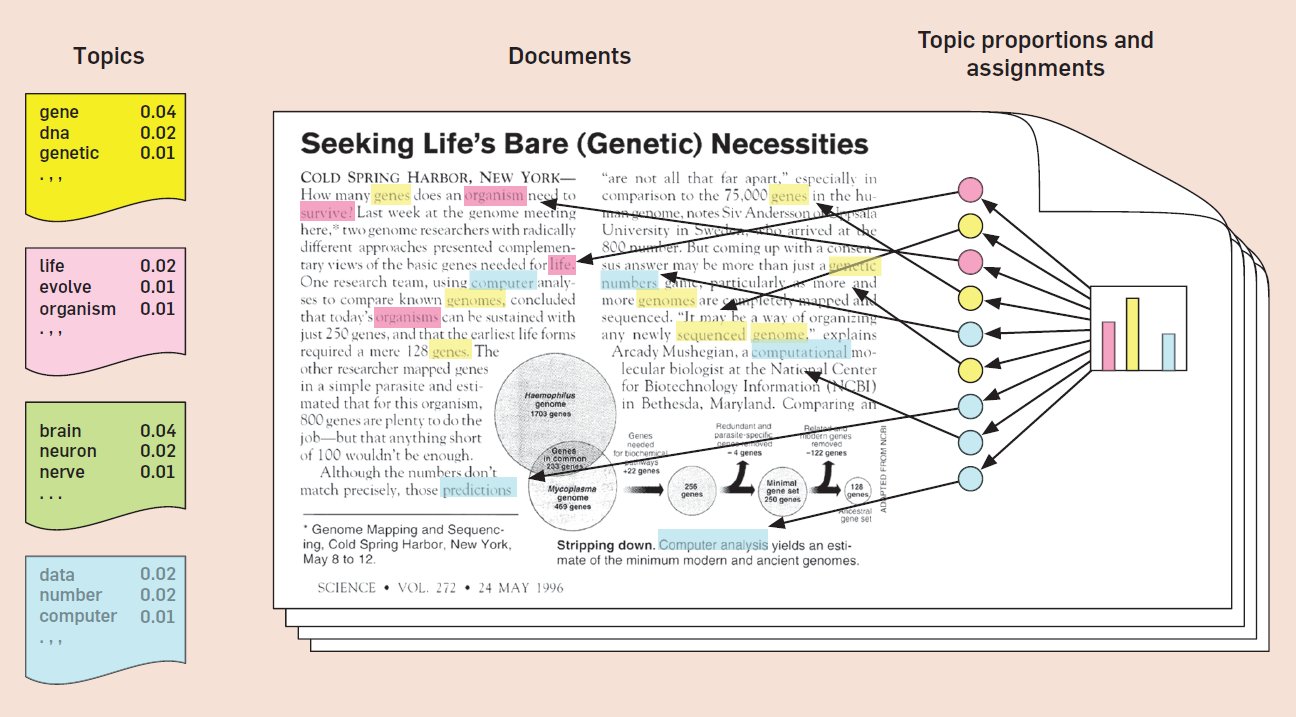
\includegraphics{images/blei2012.png}
\caption{LDA}
\end{figure}

Lo interesante de esta manera de operativizar los temas, es que cada tópico puede ser entendido como un campo semántico, un conjunto de palabras que suelen correlacionar en distintos documentos. Luego, en el momento del análisis de estos resultados, buscaremos inferir un tema a partir de las palabras que más contribuyen a cada tópico. E.g., podríamos inferir de un tópico en el que contribuyen fuertemente los términos ``venta,'' ``producto'' y ``comprador'' al tema ``comercio.''
Según uno de los autores del modelo, la interpretabilidad de la mayoría de los temas es el resultado de ``la estructura estadística del lenguaje y cómo interactúa con los supuestos probabilísticos específicos de LDA'' (D. Blei, 2012, p.~79).

A la vez, las palabras no son exclusivas de un tópico sino que cruzan todos los tópicos con una ``contribución'' relativa. Esto es justamente lo que nos interesa ya queremos comparar distintas maneras de ``contextualizar'' al mismo término (``big data'') a través de distintos tópicos, caracterizados por el uso de ciertas otras palabras.

\hypertarget{aplicar-lda}{%
\subsection{Aplicar LDA}\label{aplicar-lda}}

Vamos a construir el modelo con la función \texttt{LDA}. Una decisión importante, que debe ser introducida como un parámetro para realizar los análisis, es el número de tópicos a generar. Empecemos por un número criterioso, rápido para testear, y fácil de examinar, y volvamos sobre este problema.

\begin{Shaded}
\begin{Highlighting}[]
\FunctionTok{library}\NormalTok{(topicmodels)}
\NormalTok{k\_topics }\OtherTok{\textless{}{-}} \DecValTok{6} \CommentTok{\# numero de topicos}
\NormalTok{noticias\_tm }\OtherTok{\textless{}{-}}\NormalTok{ topicmodels}\SpecialCharTok{::}\FunctionTok{LDA}\NormalTok{(}
\NormalTok{  noticias\_dtm, }\CommentTok{\# vector de terminos por documentos}
  \AttributeTok{k =}\NormalTok{ k\_topics, }\CommentTok{\# cantidad de topicos}
  \AttributeTok{method =} \StringTok{"Gibbs"}\NormalTok{, }\CommentTok{\# metodo de sampleo de los documentos}
  \AttributeTok{control =} \FunctionTok{list}\NormalTok{(}\AttributeTok{seed =} \DecValTok{1}\SpecialCharTok{:}\DecValTok{5}\NormalTok{, }\AttributeTok{nstart=}\DecValTok{5}\NormalTok{, }\AttributeTok{verbose=}\DecValTok{1000}\NormalTok{))}
\end{Highlighting}
\end{Shaded}

\begin{Shaded}
\begin{Highlighting}[]
\NormalTok{noticias\_tm}
\end{Highlighting}
\end{Shaded}

\begin{verbatim}
## A LDA_Gibbs topic model with 6 topics.
\end{verbatim}

Ahora vamos a exportar los resultados en los 2 formatos que nos interesa explorar, utilizando la función \texttt{tidy}, y especificando la qué probabilidades que nos interesan:

\begin{itemize}
\tightlist
\item
  \textbf{beta}: probabilidad \emph{topico x palabra};
\item
  \textbf{gamma}: probabilidad \emph{topico x documento};
\end{itemize}

\begin{Shaded}
\begin{Highlighting}[]
\NormalTok{noticias\_tm\_beta }\OtherTok{\textless{}{-}} \FunctionTok{tidy}\NormalTok{(noticias\_tm, }\AttributeTok{matrix =} \StringTok{"beta"}\NormalTok{)}
\NormalTok{noticias\_tm\_gamma }\OtherTok{\textless{}{-}} \FunctionTok{tidy}\NormalTok{(noticias\_tm, }\AttributeTok{matrix =} \StringTok{"gamma"}\NormalTok{)}
\FunctionTok{glimpse}\NormalTok{(noticias\_tm\_beta)}
\end{Highlighting}
\end{Shaded}

\begin{verbatim}
## Rows: 41,088
## Columns: 3
## $ topic <int> 1, 2, 3, 4, 5, 6, 1, 2, 3, 4, 5, 6, 1, 2, 3, 4, 5, 6, 1, 2, 3, 4, 5, 6, 1, 2, 3, ~
## $ term  <chr> "dato", "dato", "dato", "dato", "dato", "dato", "información", "información", "in~
## $ beta  <dbl> 5.639872e-02, 1.606219e-05, 3.284946e-04, 1.830228e-05, 1.280606e-05, 1.593676e-0~
\end{verbatim}

\begin{Shaded}
\begin{Highlighting}[]
\FunctionTok{glimpse}\NormalTok{(noticias\_tm\_gamma)}
\end{Highlighting}
\end{Shaded}

\begin{verbatim}
## Rows: 600
## Columns: 3
## $ document <chr> "41", "51", "6", "23", "65", "77", "57", "99", "60", "95", "32", "56", "92", "~
## $ topic    <int> 1, 1, 1, 1, 1, 1, 1, 1, 1, 1, 1, 1, 1, 1, 1, 1, 1, 1, 1, 1, 1, 1, 1, 1, 1, 1, ~
## $ gamma    <dbl> 0.57725694, 0.46291667, 0.54157858, 0.31994645, 0.45619492, 0.07407407, 0.3450~
\end{verbatim}

\hypertarget{interpretar-el-modelo}{%
\section{Interpretar el modelo}\label{interpretar-el-modelo}}

Los resultados arrojados por el modelo pueden ser útiles para inferir tópicos. No obstante, esto implica un proceso iterativo de interpretación por parte del investigador, que incluye varios momentos:

\begin{enumerate}
\def\labelenumi{\arabic{enumi}.}
\tightlist
\item
  etiquetado manual y organización de los tópicos;
\item
  análisis de contenido;
\item
  validación;
\end{enumerate}

Al igual que en los diseños cualitativos debemos tener en consideración 2 cuestiones: (1) que las distintas tareas y momentos del análisis no son secuenciales sino más bien iterativos, y que constantemente iremos tomando decisiones que afectan (hacia adelante) y que informan (hacia atras) a otros momentos; (2) que todas estas decisiones serán mas claras y robustas si son producto del consenso entre distintos analistas que trabajan en forma autónoma y que documentan e intercambian la razones de sus decisiones (\protect\hyperlink{ref-Auerbach2003}{Auerbach and Silverstein 2003}).
No obstante, para todos los momentos que siguen vamos a asumir una \emph{escala pequeña} de investigación, es decir, donde las tareas puedan ser llevadas por 1 solo investigador. Cuando la investigación cuenta con recursos (humanos) suficientes se pueden plantear estrategias mucho más complejas para cada momento\footnote{Por ejemplo, \protect\hyperlink{ref-Chang2009}{Chang et al.} (\protect\hyperlink{ref-Chang2009}{2009}) diseñaron una serie de pruebas (humanas) rápidas para evaluar la coherencia de los tópicos, como por ejemplo, incluir términos extraños en un tópico para ver si un interprete podía identificarlo. Si te interesa esto, no te pierdas \href{https://www.youtube.com/watch?v=ZQLiDh1NJK4\&list=UUIXpjlxPL5Ow8rPO_gOHISQ\&index=83}{la presentación de los autores}.}, generando así resultados más confiables y robustos.

\hypertarget{etiquetado-manual-y-organizaciuxf3n-de-los-tuxf3picos}{%
\subsection{Etiquetado manual y organización de los tópicos}\label{etiquetado-manual-y-organizaciuxf3n-de-los-tuxf3picos}}

El etiquetado no es un proceso distinto al de la codificación cualitativa, es decir, a la interpretación interativa de ideas y expresiones repetidas y la imputación de un código o etiqueta que lo identifica.

En términos de \emph{codeo}, preparar los datos para esta tarea es muy fácil: simplemente listamos los términos que más contribuyen a cada tópico.

\begin{Shaded}
\begin{Highlighting}[]
\NormalTok{noticias\_tm\_beta }\SpecialCharTok{\%\textgreater{}\%} \CommentTok{\# principales términos en cada tópico}
  \FunctionTok{group\_by}\NormalTok{(topic) }\SpecialCharTok{\%\textgreater{}\%}
  \FunctionTok{top\_n}\NormalTok{(}\DecValTok{15}\NormalTok{) }\SpecialCharTok{\%\textgreater{}\%}
  \FunctionTok{ungroup}\NormalTok{() }\SpecialCharTok{\%\textgreater{}\%}
  \FunctionTok{arrange}\NormalTok{(topic, }\SpecialCharTok{{-}}\NormalTok{beta) }\SpecialCharTok{\%\textgreater{}\%} \CommentTok{\# vamos a mostrarlo como grafico}
  \FunctionTok{ggplot}\NormalTok{(}\FunctionTok{aes}\NormalTok{(}\AttributeTok{x=}\FunctionTok{reorder}\NormalTok{(term, (beta)),}\AttributeTok{y=}\NormalTok{beta)) }\SpecialCharTok{+} 
    \FunctionTok{geom\_col}\NormalTok{() }\SpecialCharTok{+}
    \FunctionTok{facet\_wrap}\NormalTok{(}\SpecialCharTok{\textasciitilde{}}\NormalTok{topic, }\AttributeTok{scales =} \StringTok{"free\_y"}\NormalTok{) }\SpecialCharTok{+}
  \FunctionTok{coord\_flip}\NormalTok{()}
\end{Highlighting}
\end{Shaded}

\includegraphics{curso-intro-r_files/figure-latex/unnamed-chunk-60-1.pdf}

El objetivo del análisis que haremos (manualmente) sobre estos datos es el de evaluar si hay un campo coherente de palabras en cada tópico, para luego asignarle una etiqueta que lo describa. En tanto estas son todas inferencias nuestras, en el mejor de los casos, guidados por nuestro conocimiento teórico del fenómeno, nos ubicamos en el plano de las hipótesis.

Veamos esto con nuestros datos, tendiendo en mente el criterio de construcción del corpus (noticias que incluyen ``big data''):

\begin{itemize}
\tightlist
\item
  Tópico 1: dato, información, empresa, usuario, millón, personas e internet son nociones que nos remiten a redes sociales y plataformas. Esta es una interpretación (hipotética) de las palabras en relación a los conceptos de la datificación y el big data social (\protect\hyperlink{ref-VanDijck2014}{Dijck 2014});
\item
  Tópico 2: campañana, político, gobierno, elección nos permiten inferir el campo de las elecciones políticas;
\item
  Tópico 3: bigdata, saber, entender, tiempo, estadística y conocimiento nos permiten suponer que se trata de la ``promesa epistémica'' del big data, es decir, de su vinculación con la generación de conocimiento novedoso (\protect\hyperlink{ref-Becerra2018}{Becerra 2018});
\item
  Tópico 4: vida, mismo, nuevo, humano son expresiones esperables en artículos críticos de los avances tecnológicos;
\item
  Tópico 5: negocio, tecnología, trabajo, innovación son términos que podrían corresponder a noticias sobre el mercado laboral y las empresas;
\item
  Tópico 6: equipo, tiempo, sensor, ciudad no parece permitirnos inferir un campo semántico muy coherente sino más bien un conjunto de artículos de áreas diversas en las que ha impactado la datificación.
\end{itemize}

Vamos a escribir estas etiquetas en un array de nombres de tópicos, por si necesitamos incluirlos en futuros gráficos como etiquetas:

\begin{Shaded}
\begin{Highlighting}[]
\NormalTok{topicos\_nombres }\OtherTok{\textless{}{-}} \FunctionTok{rbind}\NormalTok{( }
  \FunctionTok{c}\NormalTok{(}\AttributeTok{topic =} \DecValTok{1}\NormalTok{ , }\AttributeTok{nombre =} \StringTok{"1. Redes sociales"}\NormalTok{),}
  \FunctionTok{c}\NormalTok{(}\AttributeTok{topic =} \DecValTok{2}\NormalTok{ , }\AttributeTok{nombre =} \StringTok{"2. Elecciones"}\NormalTok{),}
  \FunctionTok{c}\NormalTok{(}\AttributeTok{topic =} \DecValTok{3}\NormalTok{ , }\AttributeTok{nombre =} \StringTok{"3. Conocimiento"}\NormalTok{),}
  \FunctionTok{c}\NormalTok{(}\AttributeTok{topic =} \DecValTok{4}\NormalTok{ , }\AttributeTok{nombre =} \StringTok{"4. Críticas"}\NormalTok{),}
  \FunctionTok{c}\NormalTok{(}\AttributeTok{topic =} \DecValTok{5}\NormalTok{ , }\AttributeTok{nombre =} \StringTok{"5. Negocios y trabajo"}\NormalTok{),}
  \FunctionTok{c}\NormalTok{(}\AttributeTok{topic =} \DecValTok{6}\NormalTok{ , }\AttributeTok{nombre =} \StringTok{"6. Datificación"}\NormalTok{)}
\NormalTok{) }\SpecialCharTok{\%\textgreater{}\%} \FunctionTok{as\_tibble}\NormalTok{() }\SpecialCharTok{\%\textgreater{}\%} \FunctionTok{mutate}\NormalTok{(}\AttributeTok{topic=}\FunctionTok{as.integer}\NormalTok{(topic))}
\end{Highlighting}
\end{Shaded}

Es importante tener en cuenta que no siempre todos los tópicos presentarán un campo semántico coherente: en muchos casos pueden referir a regularidades propias del tipo de comunicación que estamos analizando (e.g., palabras que remiten a una interacción por parte del usuario, si es que estamos trabajando con contenido tomado de páginas interactivas), o una mixtura de palabras tal que en lugar de permitirnos inferir un campo unívoco, nos resulte incoherente.

Luego, debemos organizar nuestros tópicos:

\begin{itemize}
\item
  \textbf{¿Descartamos tópicos irrelevantes?}: Más allá de los tópicos incoherentes o para los que un campo semántico no es tan evidente, podemos decidir filtrar otros tópicos en vistas de su (ir)relevancia para nuestra pregunta teórica. En nuestro caso, todos los tópicos parecen incluir aspectos sociales en los que el big data interviene
\item
  \textbf{¿Agrupar tópicos?}: Generalmente, en una codificación cualitativa, el proceso se repite iterativamente, haciendo inferencias cada vez más generales (mayor abstracción) y coordinadas (mayor coherencia), lo que nos permite pasar de los códigos a los temas y argumentos. El modelo LDA no tiene esa estructura jerárquica, pero nosotros podemos agrupar o colapsar tópicos en temáticas más generales. Esto es casi siempre necesario cuando trabajamos con un K elevado.
\end{itemize}

\hypertarget{anuxe1lisis-de-contenido-muestreo-cualitativo}{%
\subsection{Análisis de contenido (muestreo cualitativo)}\label{anuxe1lisis-de-contenido-muestreo-cualitativo}}

Dados los objetivos de nuestra investigación -indagar las distintas maneras en que se tematiza al big data en la prensa-, no podemos quedarnos con estos resultados que, en el mejor de los casos, son una de tantas clasificación probables. Más bien, nos interesa hacer un \emph{análisis de contenido} de los documentos en relación a cada tópico (\protect\hyperlink{ref-Krippendorff2004}{Krippendorff 2004}), no sólo para aclarar las etiquetas dadas, sino también para responder a nuestras preguntas de investigación. Este tipo de análisis, en este momento de la exploración, nos permitirá comprender los contextos semánticos en los que se definen las palabras de nuestros tópicos. Para ello, conviene tener preguntas teóricamente guiadas, como por ejemplo: ¿con qué fines se asocia al big data? ¿se lo define explicitamente o se lo da por supuesto? ¿qué actores sociales están involucrados?

En este momento sólo usaremos R para seleccionar documentos de cada tópico (construir una muestra) para su posterior análisis.
Trabajaremos estas muestras manualmente en otro entorno o software destinado al análisis cualitativo o \href{https://es.wikipedia.org/wiki/Programa_para_el_an\%C3\%A1lisis_cualitativo_asistido_por_computador}{CAQDAS}.
(Aunque existe una implementación básica de una interfaz como la de otros CAQDAS en R: RDQA (R package for Qualitative Data Analysis), \url{https://rqda.r-forge.r-project.org/}).

Una forma muy básica de construir esta muestra puede ser simplemente identificar aquellos documentos que tienen mayor probabilidad en cada tópico, a partir de \texttt{noticias\_tm\_gamma}. Asumamos que con 10 documentos podemos empezar nuestros análisis, aunque recordemos que en \emph{muestreos teóricos} (cualitativos), este número no es fijo sino que se llega por un proceso de exploración:

\begin{quote}
El muestreo teórico se realiza para descubrir categorías y sus propiedades, y para sugerir las interrelaciones dentro de una teoría. El muestreo estadístico se realiza para obtener evidencia precisa sobre distribuciones de una población entre categorías, que pueden ser utilizadas en descripciones o verificaciones (Glaser y Strauss, 1967: 62). Por el muestreo teórico el investigador selecciona casos a estudiar según su potencial para ayudar a refinar o expandir los conceptos o teorías ya desarrollados. La «saturación teórica» significa que agregar nuevos casos no representará hallar información adicional por medio de la cual el investigador pueda desarrollar nuevas propiedades de las categorías. \protect\hyperlink{ref-Gialdino2006}{Gialdino} (\protect\hyperlink{ref-Gialdino2006}{2006})\footnote{Para una discusión de esta idea: \protect\hyperlink{ref-Martinez-Salgado2012}{Martínez-Salgado} (\protect\hyperlink{ref-Martinez-Salgado2012}{2012})}
\end{quote}

\begin{Shaded}
\begin{Highlighting}[]
\NormalTok{noticias\_tm\_gamma }\SpecialCharTok{\%\textgreater{}\%} 
  \FunctionTok{group\_by}\NormalTok{(topic) }\SpecialCharTok{\%\textgreater{}\%}
  \FunctionTok{slice\_max}\NormalTok{(gamma, }\AttributeTok{n=}\DecValTok{10}\NormalTok{)}
\end{Highlighting}
\end{Shaded}

Sin embargo, esto supondría un riesgo. Consideremos la manera en que se distribuye la probabilidad de cada tópico por documento, observando los primeros documentos de nuestro corpus:

\begin{Shaded}
\begin{Highlighting}[]
\NormalTok{noticias\_tm\_gamma }\SpecialCharTok{\%\textgreater{}\%} \FunctionTok{filter}\NormalTok{(document }\SpecialCharTok{\%in\%} \FunctionTok{c}\NormalTok{(}\DecValTok{1}\SpecialCharTok{:}\DecValTok{20}\NormalTok{)) }\SpecialCharTok{\%\textgreater{}\%}
  \FunctionTok{ggplot}\NormalTok{(}\FunctionTok{aes}\NormalTok{(}\AttributeTok{x=}\NormalTok{document,}\AttributeTok{y=}\NormalTok{gamma,}\AttributeTok{label=}\NormalTok{topic,}\AttributeTok{color=}\FunctionTok{as.factor}\NormalTok{(topic))) }\SpecialCharTok{+}
  \FunctionTok{geom\_text}\NormalTok{(}\AttributeTok{size=}\DecValTok{5}\NormalTok{, }\AttributeTok{show.legend =} \ConstantTok{FALSE}\NormalTok{) }\SpecialCharTok{+}
  \FunctionTok{coord\_flip}\NormalTok{()}
\end{Highlighting}
\end{Shaded}

\includegraphics{curso-intro-r_files/figure-latex/unnamed-chunk-63-1.pdf}

En algunos documentos se observa una clara preminencia de un tópico, mientras que en otros esta distribución es más pareja (e.g., documentos \#10 y \#12). Si nos quedásemos sólo con el tópico que más alto puntúa en cada documento para asignarlos a una muestra, podríamos perder la chance de observar de qué manera algún tópico menos predominante se contextualiza. Para ello conviene construir nuestra muestra para que incluya tanto documentos con los valores más altos de afinidad, y otros seleccionados al azar que incluyan al tópico en un cierto umbral de relevancia. Esta es una decisión que deberemos considerar para otros momentos en los que querramos referir al conjunto de documentos que creemos relevante para un tópico.

\begin{Shaded}
\begin{Highlighting}[]
\NormalTok{muestra\_mixta\_1 }\OtherTok{\textless{}{-}}\NormalTok{ noticias\_tm\_gamma }\SpecialCharTok{\%\textgreater{}\%} 
  \FunctionTok{group\_by}\NormalTok{(topic) }\SpecialCharTok{\%\textgreater{}\%}
  \FunctionTok{slice\_max}\NormalTok{(gamma, }\AttributeTok{n=}\DecValTok{5}\NormalTok{)}
\NormalTok{muestra\_mixta\_2 }\OtherTok{\textless{}{-}}\NormalTok{ noticias\_tm\_gamma }\SpecialCharTok{\%\textgreater{}\%} 
  \FunctionTok{filter}\NormalTok{(gamma }\SpecialCharTok{\textgreater{}} \FloatTok{0.2}\NormalTok{) }\SpecialCharTok{\%\textgreater{}\%} \CommentTok{\# definimos el umbral}
  \FunctionTok{filter}\NormalTok{(}\SpecialCharTok{!}\NormalTok{document }\SpecialCharTok{\%in\%}\NormalTok{ muestra\_mixta\_1}\SpecialCharTok{$}\NormalTok{document) }\SpecialCharTok{\%\textgreater{}\%}
  \FunctionTok{group\_by}\NormalTok{(topic) }\SpecialCharTok{\%\textgreater{}\%}
  \FunctionTok{slice\_sample}\NormalTok{(}\AttributeTok{n =} \DecValTok{5}\NormalTok{)}
\NormalTok{muestra\_mixta }\OtherTok{\textless{}{-}} \FunctionTok{rbind}\NormalTok{(muestra\_mixta\_1, muestra\_mixta\_2)}
\end{Highlighting}
\end{Shaded}

\hypertarget{validaciuxf3n}{%
\subsection{Validación}\label{validaciuxf3n}}

En el momento de la validación se busca indagar cuán sólida es nuestra interpretación de los datos.

Hay diversas formas de validación pero podemos agruparlas en 2:

\begin{enumerate}
\def\labelenumi{\arabic{enumi}.}
\tightlist
\item
  validación de hipótesis con contenidos y metadatos;
\item
  validación estadística;
\end{enumerate}

La validación de hipótesis con contenido y metadatos (también llamada validación semántica intratópico y externa, respectivamente) consiste en hipotetizar cierta información presente en nuestros datos o metadatos, generalmente no analizados por nuestro modelo, para explorarla con los resultados del modelo.

Por ejemplo, en nuestra base de \texttt{noticias} tenemos algunos meta-datos con información que nuestro modelo no analizó (como la fecha de publicación de los artículos o sus títulos), de modo que podríamos usarlos para evaluar su coherencia. Naturalmente, esto deja muchas definiciones de criterios en manos del investigador y lo compromete a justificar sus decisiones.

\begin{Shaded}
\begin{Highlighting}[]
\NormalTok{noticias\_tm\_gamma }\SpecialCharTok{\%\textgreater{}\%}
  \FunctionTok{filter}\NormalTok{(}
\NormalTok{    gamma }\SpecialCharTok{\textgreater{}} \FloatTok{0.2} \CommentTok{\# vamos a incluir a todas las noticias con este \% de relevancia}
\NormalTok{    ) }\SpecialCharTok{\%\textgreater{}\%} 
  \FunctionTok{mutate}\NormalTok{(}
    \AttributeTok{id=}\FunctionTok{as.integer}\NormalTok{(document), }\CommentTok{\# modificamos los nombres de columnas para dp hacer join}
    \AttributeTok{topic=}\FunctionTok{as.integer}\NormalTok{(topic)}
\NormalTok{    ) }\SpecialCharTok{\%\textgreater{}\%}
  \FunctionTok{left\_join}\NormalTok{(}\AttributeTok{x =}\NormalTok{ ., }\AttributeTok{y =}\NormalTok{ noticias, }\AttributeTok{by=}\StringTok{"id"}\NormalTok{) }\SpecialCharTok{\%\textgreater{}\%} \CommentTok{\# agregamos los metadatos de noticias}
  \FunctionTok{left\_join}\NormalTok{(topicos\_nombres, }\AttributeTok{by=}\StringTok{"topic"}\NormalTok{)  }\SpecialCharTok{\%\textgreater{}\%} \CommentTok{\# agregamos los nombres de los topicos}
  \FunctionTok{group\_by}\NormalTok{(nombre, }\AttributeTok{month =}\NormalTok{ lubridate}\SpecialCharTok{::}\FunctionTok{floor\_date}\NormalTok{(fecha, }\AttributeTok{unit =} \StringTok{"month"}\NormalTok{)) }\SpecialCharTok{\%\textgreater{}\%} \CommentTok{\# agrupamos las noticias por meses}
  \FunctionTok{summarize}\NormalTok{(}\AttributeTok{n=}\FunctionTok{n}\NormalTok{()) }\SpecialCharTok{\%\textgreater{}\%}
  \FunctionTok{ggplot}\NormalTok{( }\FunctionTok{aes}\NormalTok{(}\AttributeTok{x =}\NormalTok{ month, }\AttributeTok{y =}\NormalTok{ n, }\AttributeTok{color=}\NormalTok{nombre)) }\SpecialCharTok{+}
  \FunctionTok{geom\_line}\NormalTok{()}\SpecialCharTok{+}
  \FunctionTok{scale\_x\_date}\NormalTok{(}\AttributeTok{date\_breaks =} \StringTok{"3 months"}\NormalTok{, }\AttributeTok{date\_labels =} \StringTok{"\%m/\%y"}\NormalTok{) }\SpecialCharTok{+}
  \FunctionTok{theme}\NormalTok{(}\AttributeTok{axis.text.x =} \FunctionTok{element\_text}\NormalTok{(}\AttributeTok{angle =} \DecValTok{90}\NormalTok{, }\AttributeTok{vjust =} \FloatTok{0.5}\NormalTok{, }\AttributeTok{hjust=}\DecValTok{1}\NormalTok{))}
\end{Highlighting}
\end{Shaded}

\includegraphics{curso-intro-r_files/figure-latex/unnamed-chunk-65-1.pdf}

Por caso, en relación al tópico de las elecciones políticas, vemos un pico de noticias en los últimos meses de 2017 y principios del 2018, en el que se desarrollaron las \href{https://es.wikipedia.org/wiki/Elecciones_legislativas_de_Argentina_de_2017}{elecciones legislativas argentinas} y se conoció la explotación de datos de \href{https://es.wikipedia.org/wiki/Cambridge_Analytica\#Campa\%C3\%B1a_de_Mauricio_Macri}{Facebook por parte de Cambridge Analytica}. Se debe notar que aquí introducimos un nuevo supuesto: que la manera en que hemos construído nuestra muestra habilita a un análisis de frecuencia.

A la vez, este momento de validación puede dar inicio a exploraciones heurísticas muy interesantes. Por ejemplo, en nuestra investigación sobre el tratamiento del big data por parte de la prensa digital, buscamos comparar el tratamiento del big data a través de estos tópicos en 3 niveles: artículos, oraciones que incluían los términos ``big data,'' y las fotos que acompañaban el artículo.

Por su parte, la validación estadística busca medir cuán confiable es el modelo, aunque \textbf{solamente} en términos de cuán consistentes son sus resultados.

\emph{Perplexity} es la medida más usada en este tipo de pruebas. Esta es una métrica que resulta de una prueba tipo \emph{held-out likelihood} en los que, una vez entrenado el modelo \emph{con ciertos parámetros}, se utiliza para predecir los tópicos de documentos ``nuevos'' para el modelo, es decir, documentos que no eran parte del corpus con el que se entrenó. Volveremos sobre este diseño en el próximo capítulo con más detalle.

Por ahora, nos interesa observar que este tipo de pruebas es mayormente útil para estimar distintos modelos con diferentes parámetros. En este tutorial hemos utilizado sólo 2 inputs: el número de tópicos (K) y nuestro corpus.
En lo que sigue vamos a separar algunos documentos de nuestro corpus para tener documentos ``nuevos'' (subseteamos los primeros 10); luego, vamos a vamos a entrenar varios TM con distintos valores de K; y finalmente vamos a graficar los resultados de las pruebas de perplexity.

\begin{Shaded}
\begin{Highlighting}[]
\CommentTok{\# atención: aquí vamos a entrenar 5 veces el modelo LDA. }
\CommentTok{\# este código puede ser computacionalmente pesado y lento.}
\NormalTok{posibles\_k }\OtherTok{\textless{}{-}} \FunctionTok{c}\NormalTok{(}\DecValTok{5}\NormalTok{, }\DecValTok{10}\NormalTok{, }\DecValTok{20}\NormalTok{, }\DecValTok{50}\NormalTok{, }\DecValTok{100}\NormalTok{)}
\NormalTok{comparar\_posibles\_k }\OtherTok{\textless{}{-}}\NormalTok{ posibles\_k }\SpecialCharTok{\%\textgreater{}\%}
  \FunctionTok{map}\NormalTok{(LDA, }
      \AttributeTok{x =}\NormalTok{ noticias\_dtm[}\SpecialCharTok{{-}}\FunctionTok{c}\NormalTok{(}\DecValTok{1}\SpecialCharTok{:}\DecValTok{10}\NormalTok{),], }\CommentTok{\# subseteamos todos los documentos menos los primeros 10}
      \AttributeTok{method =} \StringTok{"Gibbs"}\NormalTok{,}
      \AttributeTok{control =} \FunctionTok{list}\NormalTok{(}\AttributeTok{seed =} \DecValTok{1}\SpecialCharTok{:}\DecValTok{5}\NormalTok{, }\AttributeTok{nstart=}\DecValTok{5}\NormalTok{, }\AttributeTok{verbose=}\DecValTok{1000}\NormalTok{))}
\end{Highlighting}
\end{Shaded}

\begin{Shaded}
\begin{Highlighting}[]
\FunctionTok{tibble}\NormalTok{(}\AttributeTok{k =}\NormalTok{ posibles\_k,}
           \AttributeTok{perplex =} \FunctionTok{map\_dbl}\NormalTok{(comparar\_posibles\_k, perplexity, }
                             \AttributeTok{newdata=}\NormalTok{noticias\_dtm[}\FunctionTok{c}\NormalTok{(}\DecValTok{1}\SpecialCharTok{:}\DecValTok{10}\NormalTok{),], }
                             \AttributeTok{estimate\_theta=}\ConstantTok{FALSE}\NormalTok{)) }\SpecialCharTok{\%\textgreater{}\%}
  \FunctionTok{ggplot}\NormalTok{(}\FunctionTok{aes}\NormalTok{(k, perplex)) }\SpecialCharTok{+}
  \FunctionTok{geom\_point}\NormalTok{() }\SpecialCharTok{+}
  \FunctionTok{geom\_line}\NormalTok{()}
\end{Highlighting}
\end{Shaded}

\includegraphics{curso-intro-r_files/figure-latex/unnamed-chunk-71-1.pdf}

Dado que perplexity es una medida de inconsistencia, conviene un valor más bajo. Generalmente estos valores se consiguen a un K mayor. En este ejemplo vemos un caso extremo e improbable, en el que suponemos más tópicos (K=100) que documentos en el corpus de entrenamiento (90). Veamos cómo se ven algunos tópicos de este último modelo, en términos de distribuciones probables de palabras (beta):

\begin{Shaded}
\begin{Highlighting}[]
\NormalTok{comparar\_posibles\_k[[}\DecValTok{4}\NormalTok{]]}
\end{Highlighting}
\end{Shaded}

\begin{verbatim}
## A LDA_Gibbs topic model with 50 topics.
\end{verbatim}

\begin{Shaded}
\begin{Highlighting}[]
\FunctionTok{tidy}\NormalTok{(comparar\_posibles\_k[[}\DecValTok{4}\NormalTok{]], }\AttributeTok{matrix =} \StringTok{"beta"}\NormalTok{) }\SpecialCharTok{\%\textgreater{}\%}
  \FunctionTok{filter}\NormalTok{(topic }\SpecialCharTok{\%in\%} \FunctionTok{c}\NormalTok{(}\DecValTok{1}\SpecialCharTok{:}\DecValTok{15}\NormalTok{)) }\SpecialCharTok{\%\textgreater{}\%}
  \FunctionTok{group\_by}\NormalTok{(topic) }\SpecialCharTok{\%\textgreater{}\%}
  \FunctionTok{top\_n}\NormalTok{(}\DecValTok{10}\NormalTok{) }\SpecialCharTok{\%\textgreater{}\%}
  \FunctionTok{group\_by}\NormalTok{(topic) }\SpecialCharTok{\%\textgreater{}\%}
  \FunctionTok{summarize}\NormalTok{(}\AttributeTok{terminos =} \FunctionTok{paste}\NormalTok{(term, }\AttributeTok{collapse =} \StringTok{" , "}\NormalTok{) }\SpecialCharTok{\%\textgreater{}\%}\NormalTok{ stringr}\SpecialCharTok{::}\FunctionTok{str\_sub}\NormalTok{(}\AttributeTok{string =}\NormalTok{ ., }\AttributeTok{start =} \DecValTok{1}\NormalTok{, }\AttributeTok{end =} \DecValTok{80}\NormalTok{))}
\end{Highlighting}
\end{Shaded}

\begin{verbatim}
## Selecting by beta
\end{verbatim}

\begin{verbatim}
## # A tibble: 15 x 2
##    topic terminos                                                                          
##    <int> <chr>                                                                             
##  1     1 "contenido , necesitar , resultado , mercadeo , cuarto , evaluar , ola , presente"
##  2     2 "semiótica , palabra , punto , memorable , escribir , humanidad , literario , est"
##  3     3 "tecnología , investigación , describir , población , marcha , preciso , impresio"
##  4     4 "parecer , crear , minuto , próximo , situación , coincidir , relacionado , adapt"
##  5     5 "millón , consulta , informar , llamar , valioso , plan , sesión , caída , detall"
##  6     6 "equipo , béisbol , deporte , partido , alemán , jugador , nacimiento , posible ,"
##  7     7 "estadística , medir , social , estadístico , técnico , encuesta , cuestión , met"
##  8     8 "carrera , obtener , resolver , cálculo , década , alcance , ocupar , regulación "
##  9     9 "innovación , contenido , lector , cultural , patrón , gusto , recomendación , in"
## 10    10 "experimentación , humano , vida , relación , condición , creer , encarpetado , c"
## 11    11 "seguridad , humano , negocio , tecnología , nivel , recurso , innovación , cambi"
## 12    12 "historia , lucha , posición , relato , depresión , represión , presente , poder "
## 13    13 "fuente , provincia , judicial , autor , cosa , físico , venir , jefe , fin , cue"
## 14    14 "universidad , peso , asesorar , pese , masivo , incorporar , brasileño , partici"
## 15    15 "celular , producción , real , elaborar , década , obligatorio , publicidad , div"
\end{verbatim}

\begin{Shaded}
\begin{Highlighting}[]
\NormalTok{comparar\_posibles\_k[[}\DecValTok{5}\NormalTok{]]}
\end{Highlighting}
\end{Shaded}

\begin{verbatim}
## A LDA_Gibbs topic model with 100 topics.
\end{verbatim}

\begin{Shaded}
\begin{Highlighting}[]
\FunctionTok{tidy}\NormalTok{(comparar\_posibles\_k[[}\DecValTok{5}\NormalTok{]], }\AttributeTok{matrix =} \StringTok{"beta"}\NormalTok{) }\SpecialCharTok{\%\textgreater{}\%}
  \FunctionTok{filter}\NormalTok{(topic }\SpecialCharTok{\%in\%} \FunctionTok{c}\NormalTok{(}\DecValTok{1}\SpecialCharTok{:}\DecValTok{15}\NormalTok{)) }\SpecialCharTok{\%\textgreater{}\%}
  \FunctionTok{group\_by}\NormalTok{(topic) }\SpecialCharTok{\%\textgreater{}\%}
  \FunctionTok{top\_n}\NormalTok{(}\DecValTok{10}\NormalTok{) }\SpecialCharTok{\%\textgreater{}\%}
  \FunctionTok{group\_by}\NormalTok{(topic) }\SpecialCharTok{\%\textgreater{}\%}
  \FunctionTok{summarize}\NormalTok{(}\AttributeTok{terminos =} \FunctionTok{paste}\NormalTok{(term, }\AttributeTok{collapse =} \StringTok{" , "}\NormalTok{) }\SpecialCharTok{\%\textgreater{}\%}\NormalTok{ stringr}\SpecialCharTok{::}\FunctionTok{str\_sub}\NormalTok{(}\AttributeTok{string =}\NormalTok{ ., }\AttributeTok{start =} \DecValTok{1}\NormalTok{, }\AttributeTok{end =} \DecValTok{80}\NormalTok{)) }
\end{Highlighting}
\end{Shaded}

\begin{verbatim}
## Selecting by beta
\end{verbatim}

\begin{verbatim}
## # A tibble: 15 x 2
##    topic terminos                                                                          
##    <int> <chr>                                                                             
##  1     1 "podés , club , sistema , propio , terrorismo , economista , comprar , secreto , "
##  2     2 "conocimiento , ciencia , contar , científico , pensamiento , física , tal , físi"
##  3     3 "establecer , básico , dirigir , fabricante , basar , agregado , guardar , organi"
##  4     4 "deporte , mundial , existir , pobreza , producir , pueblo , proceso , móvil , la"
##  5     5 "pareja , grupo , día , sensor , seguir , terrorismo , político , foto , disposit"
##  6     6 "trabajo , mensaje , sitio , crear , informe , fuerza , venir , euro , peligroso "
##  7     7 "cuadro , mundo , redes_social , marca , presidente , problema , producción , log"
##  8     8 "campaña , cuenta , conversación , necesidad , beneficio , cerrar , capacidad , r"
##  9     9 "alemán , peso , quedar , tratar , calidad , cambiar , móvil , interés , gobernad"
## 10    10 "posibilidad , argentino , tiempo , director , terrorismo , fundador , ofrecer , "
## 11    11 "joven , negocio , salud , nivel , responder , establecer , causa , cambiar , ele"
## 12    12 "información , dólar , riego , colega , compañía , mercado , derecho , serie , es"
## 13    13 "ciudad , negocio , gobierno , mensaje , buscar , electoral , activo , técnica , "
## 14    14 "patrón , actividad , paso , relato , quedar , lectura , llegar , adulto , intere"
## 15    15 "mayor , experimento , país , analizar , asesor , acceso , humanos , psicología ,"
\end{verbatim}

¿Te resultan tópicos más claros? Diferentes estudios (\protect\hyperlink{ref-Hagen2018}{Hagen} (\protect\hyperlink{ref-Hagen2018}{2018}), \protect\hyperlink{ref-Maier2018}{Maier et al.} (\protect\hyperlink{ref-Maier2018}{2018}), \protect\hyperlink{ref-Boyd-Graber2014}{Boyd-Graber, Mimno, and Newman} (\protect\hyperlink{ref-Boyd-Graber2014}{2014}), \protect\hyperlink{ref-Chang2009}{Chang et al.} (\protect\hyperlink{ref-Chang2009}{2009})) muestran que números elevandos de K, si bien son más útiles para una clasificación efectiva de documentos nuevos, no suelen dar tópicos más \emph{interpretables}, es decir, más claros en términos de distinguir los sentidos que se incluyen. De hecho, parece más bien haber una correlación negativa entre la interpretabilidad de los tópicos y medidas predictivas como perplexity! Incluso, algunos de estos estudios afirman que un K \textgreater{} 50 no es humanamente interpretable, dada la dificultad de leer los resultados sin confundir u olvidar los tópicos posibles.

¿Entonces, cómo determinar K, y con ello la validez de nuestro modelo? Bueno, por el momento parece haber sólo algunos lineamientos generales:

\begin{itemize}
\tightlist
\item
  se procede por prueba y error, buscando agregar y desagregar tópicos, maximizando el número de tópicos coherentes;
\item
  asumiendo que K debe ser lo suficiente pequeño como para que sean recordados e interpretables;
\item
  y lo suficiente grande como para evitarnos asignar documentos muy dispares al mismo grupo;
\item
  usar pruebas estadísticas entre K de ordenes muy distintos, para tener una idea de los límites del \emph{overfitting};
\end{itemize}

Finalmente, el criterio no parece ser muy distinto que el que podemos aplicar en investigación cualitativa: realizar muestreos teóricos a conciencia, transparentar nuestros criterios a la hora de inferir y tomar decisiones, explicitar el marco de sentido de nuestras interpretaciones (nuestro marco teórico y epistemológico), discutir nuestras conclusiones y buscar acuerdos, sabiendo que el sentido del análisis no es tener la última palabra sino ofrecer una interpretación razonable empíricamente fundada.

¿Es esta \emph{dependencia} en el análisis cualitativo algo negativo? Sólo si nuestro objetivo es automatizar un análisis fiable sin intervención (y costos) del trabajo humano\ldots{} pero esto también es una limitación en los objetivos del análisis, no pudiendo avanzar sobre un ejercicio clasificatorio. Más promisorio es tomar al modelado de tópicos como un primer paso, una herramienta heurística, en nuestra exploración de los datos.

\begin{quote}
\emph{Topic models must find what we know is there.} Ultimately, a topic model's trustworthiness must be determined by informed human judgments. In particular, the model must find the broad trends and facts known to be true by the practitioner of the domain. Without such support in finding the known, topic models have limited value in discovering the unknown --- i.e.~quantifying known trends or discovering unexpected ones. (\protect\hyperlink{ref-Ramage2009}{Ramage et al. 2009})
\end{quote}

\hypertarget{clasificar-automaticamente}{%
\chapter{Clasificar automaticamente}\label{clasificar-automaticamente}}

En este capítulo nos introduciremos a una técnica de ``aprendizaje supervisado.'' Nos referimos así a algoritmos que, a partir de datos que ya están clasificados o catalogados de antemano por medio de alguna variable (``datos etiquetados''), buscan inferir reglas para clasificar otros registros.
Lo interesante de este tipo tareas es que nosotros no estamos introduciendo \emph{reglas explícitas} sino que nuestro modelo resultará de registrar patrones diferenciales para las clases de datos que servimos.
Esta tarea se considera ``supervisada'' porque somos nosotros los que le indicamos previamente qué es lo que está observando/aprendiendo.

Así, por ejemplo, podríamos construir un modelo que tome una base de datos de pacientes afectados por covid-19, clasificados en ``internados en terapia intensiva'' y ``no internados en terapia intensiva,'' para estimar cuáles nuevos pacientes son de riesgo, a partir considerar otros datos en nuestro registro, tales como la edad, el género, y las condiciones clínicas.

La \emph{clasificación} no es la única tarea posible para un modelo de entrenamiento supervisado. Podríamos, por ejemplo, estar interesados en predecir el precio de un departamento en venta a partir de un modelo previamente entrenado con cientos y cientos de unidades de las que se sabe de cada una su superficie, localía, antigüedad, orientación, etc. Un modelo de este tipo, que asocie todas estas variables a un precio que queremos predecir, haría referencia a lo que llamamos \emph{regresión}. A diferencia de los modelos de clasificación, que predicen etiquetas, los modelos de regresión predicen valores numéricos contínuos.

En lo que sigue construiremos un modelo para clasificar oraciones sobre big data en positivas y negativas, a partir de un corpus de oraciones ya anotadas manualmente. Este corpus se construyó por medio de \emph{scrapping} de diferentes artículos periodísticos provenientes de diarios online argentinos. De esta manera, seguiremos explorando las posibilidades y recovecos del análisis de sentimientos, de modo que este ejercicio continúa (con otro método) lo iniciado en el capitulo 3. Como nuestro corpus es textual, aquí seguimos dentro del amplio abanico de las posibilidades del procesamiento del lenguaje natural p NLP (Natural Language Processing), de modo que veremos algunas tareas repetidas con respecto a capítulos previos.

A lo largo de este ejercicio veremos cómo:

\begin{enumerate}
\def\labelenumi{\arabic{enumi}.}
\tightlist
\item
  pre-procesar texto;
\item
  vectorizar textos;
\item
  dividir del corpus para entrenamiento y testeo;
\item
  armar el modelo de clasificación;
\item
  evaluar el modelo;
\item
  ajustar el modelo.
\end{enumerate}

A lo largo de este tutorial trabajaremos con varias librerías, que podemos instalar con el siguiente código:

\begin{Shaded}
\begin{Highlighting}[]
\FunctionTok{install.packages}\NormalTok{(}\FunctionTok{c}\NormalTok{(}\StringTok{"tidyverse"}\NormalTok{, }\StringTok{"udpipe"}\NormalTok{, }\StringTok{"tm"}\NormalTok{, }\StringTok{"tidytext"}\NormalTok{)) }\CommentTok{\# las hemos instalado en capítulos anteriores}
\FunctionTok{install.packages}\NormalTok{(}\FunctionTok{c}\NormalTok{(}\StringTok{"caTools"}\NormalTok{, }\StringTok{"caret"}\NormalTok{, }\StringTok{"randomForest"}\NormalTok{, }\StringTok{"rpart"}\NormalTok{, }\StringTok{"rpart.plot"}\NormalTok{, }\StringTok{"ROSE"}\NormalTok{)) }\CommentTok{\# las usaremos por primera vez}
\end{Highlighting}
\end{Shaded}

\hypertarget{preprocesamiento}{%
\section{Preprocesamiento}\label{preprocesamiento}}

Tal como lo realizamos en el capitulo anterior, antes de avanzar a una instancia de entrenamiento de modelo, debemos ``preparar'' los datos para que sean entendibles por la máquina. ``Preprocesamiento,'' entonces, es el conjunto de técnicas y estrategias que aplicamos sobre nuestros datos para facilitar el posterior proceso de entrenamiento de un modelo. Como vimos en el capítulo anteior, el desafío de preprocesamiento en el ámbito del lenguaje natural pasa por 2 instancias: normalizar y vectorizar los datos. De fondo, lo que nos permite este flujo es ``estructurar'' datos no-estructurados.

Empecemos por importar y observar nuestra base de datos.

\begin{Shaded}
\begin{Highlighting}[]
\FunctionTok{library}\NormalTok{(tidyverse) }\CommentTok{\# para manipular tablas}
\NormalTok{oraciones }\OtherTok{\textless{}{-}}\NormalTok{ readr}\SpecialCharTok{::}\FunctionTok{read\_csv}\NormalTok{(}\StringTok{"https://raw.githubusercontent.com/gastonbecerra/curso{-}intro{-}r/main/data/oraciones\_entrenamiento.csv"}\NormalTok{) }\SpecialCharTok{\%\textgreater{}\%} \CommentTok{\# importamos los datos}
  \FunctionTok{rename}\NormalTok{(}\AttributeTok{clase\_oracion=}\NormalTok{estado, }\AttributeTok{id=}\NormalTok{doc\_id) }
\FunctionTok{glimpse}\NormalTok{(oraciones) }\CommentTok{\# exploramos la estructura de los datos}
\end{Highlighting}
\end{Shaded}

\begin{verbatim}
## Rows: 400
## Columns: 3
## $ id            <dbl> 3578, 2300, 405, 2540, 2016, 2713, 1503, 534, 1101, 3043, 1458, 1010, 41,~
## $ oracion       <chr> "vale aclarar que bigdata es el nombre que se utiliza para describir a lo~
## $ clase_oracion <chr> "positivo", "positivo", "positivo", "positivo", "positivo", "positivo", "~
\end{verbatim}

La variable que tiene nuestra ``etiqueta'' y clasifica a cada oración es la variable \texttt{clase\_oracion}, que oscila en dos valores: positivo (generalmente, cuando la oración da cuenta de los posibles beneficios del big data) y negativo (generalmente, cuando la oración implica que el big data es un fenómeno riesgoso). Esta es la variable que buscaremos inferir en oraciones nuevas, a partir del procesamiento de las demás variables.

\begin{Shaded}
\begin{Highlighting}[]
\FunctionTok{table}\NormalTok{(oraciones}\SpecialCharTok{$}\NormalTok{clase\_oracion) }\CommentTok{\# vemos la distribución de las clasificaciones}
\end{Highlighting}
\end{Shaded}

\begin{verbatim}
## 
## negativo positivo 
##      100      300
\end{verbatim}

Como podemos observar, encontramos aquí un dataset ``desbalanceado,'' en el que una cierta clase se encuentran sobre-representada en el total de la población. Particularmente: los primeros 300 registros son oraciones positivas, mientras que los últimos 100 son negativos.
Esta proporción no debe sorprendernos si consideramos el origen del dataset: en las noticias abunda el discurso promocional del big data que lo presenta como una revolución del conocimiento con aplicaciones posibles en distintos campos de la industria y el comercio, o en el manejo de las cuestiones de gobierno, sobre aquellas noticias que ponen el foco en sus riesgos.

Este desbalanceo es uno de los tantos problemas que pueden emerger en cualquier proyecto de ciencia de datos. En muchas situaciones, la cantidad y calidad de los mismos no dependen de la responsabilidad del investigador, quien deberá pensar en estrategias para hacer su corpus más ``limpio.'' Ahondaremos en este problema más adelante.

Ahora vamos a comenzar a preprocesar los datos. En nuestro corpus, todos nuestros datos se encuentran contenidos en la variable \texttt{oracion}, que tiene expresiones del lenguaje natural. Para poder entrenar un modelo con ellas conviene empezar por reducir la complejidad de estas expresiones, por ejemplo, quedándonos con las palabras posiblemente más significativas. Aquí optamos por reconstruir las oraciones con los \emph{lemmas} de sólo algunos tipos de palabras, anotando el texto con la librería \texttt{udpipe} que hemos usado en capítulos anteriores.

\begin{Shaded}
\begin{Highlighting}[]
\CommentTok{\#install.packages("udpipe") \# instalamos la libreria}
\FunctionTok{library}\NormalTok{(udpipe) }\CommentTok{\# la cargamos}
\NormalTok{modelo\_sp }\OtherTok{\textless{}{-}}\NormalTok{ udpipe}\SpecialCharTok{::}\FunctionTok{udpipe\_download\_model}\NormalTok{(}\StringTok{\textquotesingle{}spanish\textquotesingle{}}\NormalTok{) }\CommentTok{\# descarga el modelo y guarda la referencia  }
\NormalTok{modelo\_sp}\SpecialCharTok{$}\NormalTok{file\_model }\CommentTok{\# refrencia al modelo descargado}
\NormalTok{modelo\_sp }\OtherTok{\textless{}{-}} \FunctionTok{udpipe\_load\_model}\NormalTok{(}\AttributeTok{file =}\NormalTok{ modelo\_sp}\SpecialCharTok{$}\NormalTok{file\_model) }\CommentTok{\# cargamos el modelo en memoria}
\end{Highlighting}
\end{Shaded}

\begin{Shaded}
\begin{Highlighting}[]
\NormalTok{oraciones\_anotadas }\OtherTok{\textless{}{-}} \FunctionTok{udpipe\_annotate}\NormalTok{( }
  \AttributeTok{object =}\NormalTok{ modelo\_sp, }\CommentTok{\# el modelo de idioma}
  \AttributeTok{x =}\NormalTok{ oraciones}\SpecialCharTok{$}\NormalTok{oracion, }\CommentTok{\# el texto a anotar, }
  \AttributeTok{doc\_id =}\NormalTok{ oraciones}\SpecialCharTok{$}\NormalTok{id, }\CommentTok{\# el id de cada oracion (el resultado tendrá 1 palabra x fila)}
  \AttributeTok{trace =} \DecValTok{100}
\NormalTok{  ) }\SpecialCharTok{\%\textgreater{}\%} \FunctionTok{as.data.frame}\NormalTok{(.) }\CommentTok{\# convertimos el resultado en data frame}
\end{Highlighting}
\end{Shaded}

\begin{verbatim}
## 2021-06-14 14:40:16 Annotating text fragment 1/400
## 2021-06-14 14:40:18 Annotating text fragment 101/400
## 2021-06-14 14:40:20 Annotating text fragment 201/400
## 2021-06-14 14:40:23 Annotating text fragment 301/400
\end{verbatim}

\begin{Shaded}
\begin{Highlighting}[]
\NormalTok{oraciones\_anotadas2 }\OtherTok{\textless{}{-}}\NormalTok{ oraciones\_anotadas }\SpecialCharTok{\%\textgreater{}\%} 
  \FunctionTok{filter}\NormalTok{(upos }\SpecialCharTok{\%in\%} \FunctionTok{c}\NormalTok{(}\StringTok{"ADJ"}\NormalTok{,}\StringTok{"NOUN"}\NormalTok{,}\StringTok{"VERB"}\NormalTok{) ) }\SpecialCharTok{\%\textgreater{}\%} \CommentTok{\# filtramos por tipo de palabra}
  \FunctionTok{filter}\NormalTok{(lemma }\SpecialCharTok{!=} \StringTok{"bigdata"}\NormalTok{) }\SpecialCharTok{\%\textgreater{}\%} \CommentTok{\# sacamos la expresion bigdata que estará en todas las oraciones}
  \FunctionTok{select}\NormalTok{(doc\_id, lemma) }\CommentTok{\# nos quedamos sólo con los lemmas}
\FunctionTok{glimpse}\NormalTok{(oraciones\_anotadas2)}
\end{Highlighting}
\end{Shaded}

\begin{verbatim}
## Rows: 4,719
## Columns: 2
## $ doc_id <chr> "3578", "3578", "3578", "3578", "3578", "3578", "3578", "3578", "3578", "3578", ~
## $ lemma  <chr> "valer", "aclarar", "nombre", "utilizar", "describir", "grande", "volumen", "inf~
\end{verbatim}

Con esta forma de preprocesar los datos de preprocesar los datos hemos ``perdido'' la variable que contenía la clasificación. No te preocupes, la incluiremos más adelante, cuando rearmemos las oraciones.

\hypertarget{vectorizado}{%
\section{Vectorizado}\label{vectorizado}}

La vectorización es la estrategia aquí utilizada para transformar estos datos (provenientes del lenguaje natural) en una expresión de carácter matemático, de modo que sean entendibles por una computadora. Particularmente vamos a convertir a cada oración en una fila donde contamos qué/cuantas palabras hay en relación al vocabulario total. Hay muchas formas de realizar este objetivo. Aquí optamos por realizar un conteo de palabras con las funciones de \texttt{dplyr} que ya conocemos, y trasformaremos el objeto resultante a una \emph{matriz de documentos por frecuencias} (o \emph{dtm}) con \texttt{cast\_dtm} del paquete \texttt{tidytext}.

\begin{Shaded}
\begin{Highlighting}[]
\FunctionTok{library}\NormalTok{(tidytext) }\CommentTok{\# para manejar texto}
\FunctionTok{library}\NormalTok{(tm) }\CommentTok{\# para vectorizar}
\NormalTok{or\_dtm }\OtherTok{\textless{}{-}}\NormalTok{ oraciones\_anotadas2 }\SpecialCharTok{\%\textgreater{}\%}
        \FunctionTok{count}\NormalTok{(doc\_id, lemma) }\SpecialCharTok{\%\textgreater{}\%}
\NormalTok{        tidytext}\SpecialCharTok{::}\FunctionTok{cast\_dtm}\NormalTok{(}\AttributeTok{document =}\NormalTok{ doc\_id, }\AttributeTok{term =}\NormalTok{ lemma, }\AttributeTok{value =}\NormalTok{ n)}
\NormalTok{or\_dtm}
\end{Highlighting}
\end{Shaded}

\begin{verbatim}
## <<DocumentTermMatrix (documents: 400, terms: 1649)>>
## Non-/sparse entries: 4643/654957
## Sparsity           : 99%
## Maximal term length: 23
## Weighting          : term frequency (tf)
\end{verbatim}

Las distintas palabras que se distribuyen en cada oración serán las variables que nuestro modelo va a considerar para predecir la etiqueta. Aquí podemos ir un paso más en la simplificación y en la reducción de nuestros datos para asegurarnos que los cómputos siguientes sean más rápidos. Para ellos, vamos a reducir el nivel de escasez o \emph{sparcity} de nuestros datos, eliminando aquellos términos que están menos presente a través de las oraciones, es decir, términos que mayormente registran valores de \texttt{0}. Para ello vamos a usar la función \texttt{removeSparseTerms} del paquete \texttt{tm}.

\begin{Shaded}
\begin{Highlighting}[]
\NormalTok{or\_dtm }\OtherTok{\textless{}{-}}\NormalTok{ tm}\SpecialCharTok{::}\FunctionTok{removeSparseTerms}\NormalTok{(or\_dtm, }\AttributeTok{sparse =}\NormalTok{ .}\DecValTok{98}\NormalTok{)}
\NormalTok{or\_dtm}
\end{Highlighting}
\end{Shaded}

\begin{verbatim}
## <<DocumentTermMatrix (documents: 400, terms: 92)>>
## Non-/sparse entries: 1648/35152
## Sparsity           : 96%
## Maximal term length: 23
## Weighting          : term frequency (tf)
\end{verbatim}

Ahora nuestro modelo deberá considerar un número mucho menor de variables.

\hypertarget{division-en-entrenamiento-y-testeo}{%
\section{Division en entrenamiento y testeo}\label{division-en-entrenamiento-y-testeo}}

Antes de comenzar el entrenamiento, vamos a dividir nuestra base de datos etiquetados en 2:

\begin{itemize}
\tightlist
\item
  por un lado, un conjunto de \emph{entrenamiento}, que es la porción de registros que el algoritmo va analizar observando las variables predictoras (palabras) y la etiqueta (\texttt{clase\_oracion}), para generar el modelo de clasificación. Esta porción de registros suele ser bastante más amplia.
\item
  por otro lado, un conjunto de \emph{testeo}, sobre el que vamos a aplicar el modelo para clasificar las oraciones, y con el que compararemos la predicción del modelo con la etiqueta \emph{real} de cada registro. Dicha comparación nos permitirá medir cuan fiable (\emph{accuracy}) es nuestro modelo.
\end{itemize}

Aquí vamos a usar las funciones del paquete \texttt{caTools} para realizar este procedimiento de \emph{train/test split}.

Pero antes deberemos hacer algunas transformaciones para que nuestro objeto tenga la forma requerida por \texttt{caTools}, una de las cuales es muy importante: vamos a reincluir la clase de oración (ahora como una variable de tipo factor).

\begin{Shaded}
\begin{Highlighting}[]
\FunctionTok{set.seed}\NormalTok{(}\DecValTok{100}\NormalTok{) }\CommentTok{\# seteamos una semilla, para poder reproducir los resultados}

\CommentTok{\# transformamos nuestra matriz de la manera requerida por caTools}
\NormalTok{or\_dtm2 }\OtherTok{=} \FunctionTok{as.data.frame}\NormalTok{(}\FunctionTok{as.matrix}\NormalTok{(or\_dtm))}
\FunctionTok{colnames}\NormalTok{(or\_dtm2) }\OtherTok{=} \FunctionTok{make.names}\NormalTok{(}\FunctionTok{colnames}\NormalTok{(or\_dtm2))}
\NormalTok{or\_dtm2}\SpecialCharTok{$}\NormalTok{clase\_oracion }\OtherTok{=} \FunctionTok{as.factor}\NormalTok{(oraciones}\SpecialCharTok{$}\NormalTok{clase\_oracion) }\CommentTok{\# reincluimos la clase como factor}

\FunctionTok{library}\NormalTok{(caTools) }\CommentTok{\# cargamos la librería para hacer el split}
\NormalTok{division }\OtherTok{=} \FunctionTok{sample.split}\NormalTok{(or\_dtm2}\SpecialCharTok{$}\NormalTok{clase\_oracion, }\AttributeTok{SplitRatio =} \FloatTok{0.7}\NormalTok{) }\CommentTok{\# divide 70/30}
\NormalTok{or\_train }\OtherTok{=} \FunctionTok{subset}\NormalTok{(or\_dtm2, division}\SpecialCharTok{==}\ConstantTok{TRUE}\NormalTok{) }\CommentTok{\# subconjunto de entrenamiento}
\NormalTok{or\_test }\OtherTok{=} \FunctionTok{subset}\NormalTok{(or\_dtm2, division}\SpecialCharTok{==}\ConstantTok{FALSE}\NormalTok{) }\CommentTok{\# subconjunto de testeo}
\end{Highlighting}
\end{Shaded}

Ya estamos listos para generar nuestro modelo!

\hypertarget{modelado}{%
\section{Modelado}\label{modelado}}

En lo que sigue vamos a generar distintos modelos de clasificación, utilizando distintos algoritmos.

\hypertarget{modelo-1-random-forest}{%
\subsection{Modelo 1: Random forest}\label{modelo-1-random-forest}}

\emph{Random forest} es uno de los métodos de entrenamiento de modelos más estandarizados y extendidos. Su nivel de eficacia suele ser tan bueno como su simpleza conceptual: se trata de un ``bosque'' poblado de ``árboles de decisión'' que hacen distintas preguntas a los datos, resultando en la asignación de una etiqueta.

Como su nombre lo indica, un random forest se constituye a partir del ``ensamble'' de varios árboles (de decisión). Así, la clasificación resultante de una predicción de este tipo de modelos se basa en una suerte de ``votación'' donde cada uno de los árboles del bosque emite su voto (etiqueta predicha para cada muestra) resultando electa la que mayor score haya conseguido. Este tipo de modelos de ``ensambla'' se basan en el principio de conceder mayor probabilidad de acierto a una mayoría de voces, que a la de una sola.

Para generar el modelo utilizaremos el paquete \texttt{randomForest}, con la función homónima. Si bien hay muchos parámetros, aquí utilizaremos la función de la manera más simple: indicándo tan sólo cuáles son las variables a contemplar y la variable a predecir, y cuál es la tabla con la que debe trabajar (\texttt{data=or\_train}). Para lo primero vamos a usar la notación de fórmula: \texttt{clase\_oracion\ \textasciitilde{}\ .}, donde indicamos que la variable de la izquierda (\texttt{clase\_oracion}) depende (o es \emph{función de}, \texttt{\textasciitilde{}}) las variables de la derecha, que en nuestro caso son todas las demás, de modo que las anotamos como \texttt{.}.

\begin{Shaded}
\begin{Highlighting}[]
\FunctionTok{library}\NormalTok{(randomForest) }\CommentTok{\# cargamos la librería}
\NormalTok{or\_rf }\OtherTok{=} \FunctionTok{randomForest}\NormalTok{(clase\_oracion }\SpecialCharTok{\textasciitilde{}}\NormalTok{ ., }\AttributeTok{data=}\NormalTok{or\_train) }\CommentTok{\# generar modelo}
\end{Highlighting}
\end{Shaded}

Una vez generado el modelo, es hora de validarlo con nuestros datos de testeo que, recordemos, es una parte de la base de datos \emph{anotada}, es decir, en la que cada registro ya tiene una clasificación asignada por nosotros. El sentido de esta comparación no es otro que medir la eficacia y fiabilidad del modelo. Para ello usaremos la función \texttt{predict} del paquete \texttt{stats} (generalmente precargado en la instalación de R), a la que pasaremos nuestro modelo \texttt{object=or\_rf}, junto con la base de testeo \texttt{newdata=or\_test}

\begin{Shaded}
\begin{Highlighting}[]
\NormalTok{or\_rf\_predict }\OtherTok{=} \FunctionTok{predict}\NormalTok{(}\AttributeTok{object=}\NormalTok{or\_rf, }\AttributeTok{newdata=}\NormalTok{or\_test) }\CommentTok{\# predecimos con tabla test, para evaluar contra real}
\end{Highlighting}
\end{Shaded}

El resultado de esta función es un vector que incluye las etiquetas predichas para cada registro, y que podemos comparar con las etiquetas \emph{reales}. Generalmente, en modelo clasificatorios como el nuestro, esta comparación supone la construcción de una \emph{matriz de confusión} que cruza la cantidad de registros etiquetados con cada valor \emph{real} contra la cantidad de registros etiquetados con cada valor \emph{predicho}. Podemos generar una matriz ``a mano'' con \texttt{table}, o con el paquete \texttt{caret}. Por ahora, vamos a mano:

\begin{Shaded}
\begin{Highlighting}[]
\FunctionTok{table}\NormalTok{(or\_test}\SpecialCharTok{$}\NormalTok{clase\_oracion, or\_rf\_predict) }\CommentTok{\# matriz de confusion}
\end{Highlighting}
\end{Shaded}

\begin{verbatim}
##           or_rf_predict
##            negativo positivo
##   negativo        4       26
##   positivo        6       84
\end{verbatim}

\begin{Shaded}
\begin{Highlighting}[]
\CommentTok{\# algunos datos a tener en cuenta}
\FunctionTok{nrow}\NormalTok{(or\_test) }\CommentTok{\# cantidad de registros en nuestra tabla de test}
\end{Highlighting}
\end{Shaded}

\begin{verbatim}
## [1] 120
\end{verbatim}

\begin{Shaded}
\begin{Highlighting}[]
\FunctionTok{table}\NormalTok{(or\_test}\SpecialCharTok{$}\NormalTok{clase\_oracion) }\CommentTok{\# cuantos registros en cada clase real?}
\end{Highlighting}
\end{Shaded}

\begin{verbatim}
## 
## negativo positivo 
##       30       90
\end{verbatim}

En la diagonal (descendiente) de la matriz de confusión se cuentan los casos donde la etiqueta \emph{real} y la \emph{predicha} coinciden. De aquí podemos ver que de los \texttt{120} casos, \texttt{88} fueron predichos correctamente. Es decir, un \emph{accuracy} del \texttt{0.7333333}/1. Un resultado bastante pobre!

Antes de avanzar, conviene que nos hagamos una pregunta para comprender cómo opera el modelo que hemos construído: ¿los errores del modelo son parejos? En el caso de \texttt{or\_rf\_predict}, podemos ver que las oraciones ``positivas'' tienen un ratio de error mucho menor que los ``negativos,'' o en otras palabras, que nuestro modelo no es tan bueno clasificando correctamente negativos, como lo es clasificando positivos. Esta \emph{insensibilidad} de nuestro modelo es, entre otras razones, producto de la distribución desigual, o del desbalanceo, de nuestra base.

Ahora bien, nos gustaría conocer un poco más de nuestro modelo, para entender qué reglas se generaron. ``Abrir la caja negra'' de un modelo, incluso de un modelo tan simple como el que acabamos de implementar, no es tarea fácil. Por suerte el paquete \texttt{caret} tiene algunas funciones que nos pueden dar algunas pistas. Una de ellas (\texttt{varImp} para obtener una tabla, \texttt{varImpPlot} para un gráfico) muestra la \emph{importancia} de las variables, indicando cuáles han tenido un mayor peso a la hora de determinar a qué clase corresponde un registro.

\begin{Shaded}
\begin{Highlighting}[]
\FunctionTok{library}\NormalTok{(caret)}
\FunctionTok{varImpPlot}\NormalTok{(or\_rf)}
\end{Highlighting}
\end{Shaded}

\includegraphics{curso-intro-r_files/figure-latex/unnamed-chunk-80-1.pdf}

¿Qué nos dice este gráfico? Lo que vemos ordenado de mayor a menos son las palarbas que nuestro modelo considera como más efectivas para dictaminar una predicción. Esto quiere decir que nuestro modelo tenderá a computar la presencia y o ausencia de estas palabras como dato de peso para inferir si un caso evaluado es de tal o cual clase.

Sin embargo, como mencionamos previamente analizando la matriz de confusión, nuestro modelo ha sido entrenado con una sobrerepresentación de casos positivos, por lo que sus inferencias tenderán mayoritariamente a una clasificación positiva. En otras palabras, lo que vemos aquí son las palabras que nuestro modelo considera más significativas para inferir un caso de oración positiva.

Ah! no nos olvidemos que \texttt{caret} también tiene una función que nos simplifica la construcción de una matriz de confusión, y otras métricas.

\begin{Shaded}
\begin{Highlighting}[]
\NormalTok{caret}\SpecialCharTok{::}\FunctionTok{confusionMatrix}\NormalTok{(or\_test}\SpecialCharTok{$}\NormalTok{clase\_oracion, or\_rf\_predict)}
\end{Highlighting}
\end{Shaded}

\begin{verbatim}
## Confusion Matrix and Statistics
## 
##           Reference
## Prediction negativo positivo
##   negativo        4       26
##   positivo        6       84
##                                           
##                Accuracy : 0.7333          
##                  95% CI : (0.6449, 0.8099)
##     No Information Rate : 0.9167          
##     P-Value [Acc > NIR] : 1.0000000       
##                                           
##                   Kappa : 0.0857          
##                                           
##  Mcnemar's Test P-Value : 0.0007829       
##                                           
##             Sensitivity : 0.40000         
##             Specificity : 0.76364         
##          Pos Pred Value : 0.13333         
##          Neg Pred Value : 0.93333         
##              Prevalence : 0.08333         
##          Detection Rate : 0.03333         
##    Detection Prevalence : 0.25000         
##       Balanced Accuracy : 0.58182         
##                                           
##        'Positive' Class : negativo        
## 
\end{verbatim}

Veamos si nos va mejor con otro modelo, antes de empezar a hacer ajustes.

\hypertarget{modelo-2-rpart}{%
\subsection{Modelo 2: rpart}\label{modelo-2-rpart}}

Un algoritmo alternativo es \texttt{rpart}, que se puede extender con el paquete \texttt{rpart.plot} para generar visualizaciones del modelo. El código es igual al usado con random forest.

\begin{Shaded}
\begin{Highlighting}[]
\FunctionTok{library}\NormalTok{(rpart) }\CommentTok{\# cargamos librería}
\NormalTok{or\_rpart }\OtherTok{\textless{}{-}} \FunctionTok{rpart}\NormalTok{(clase\_oracion}\SpecialCharTok{\textasciitilde{}}\NormalTok{., }\AttributeTok{data =}\NormalTok{ or\_train, }\AttributeTok{method =} \StringTok{\textquotesingle{}class\textquotesingle{}}\NormalTok{) }\CommentTok{\# generamos el modelo}
\NormalTok{or\_rpart\_predict }\OtherTok{\textless{}{-}} \FunctionTok{predict}\NormalTok{(or\_rpart, or\_test, }\AttributeTok{type =} \StringTok{\textquotesingle{}class\textquotesingle{}}\NormalTok{) }\CommentTok{\# \# predecimos con tabla test, para evaluar contra real}

\FunctionTok{confusionMatrix}\NormalTok{(or\_test}\SpecialCharTok{$}\NormalTok{clase\_oracion, or\_rpart\_predict) }\CommentTok{\# veamos como nos fue}
\end{Highlighting}
\end{Shaded}

\begin{verbatim}
## Confusion Matrix and Statistics
## 
##           Reference
## Prediction negativo positivo
##   negativo        3       27
##   positivo        5       85
##                                           
##                Accuracy : 0.7333          
##                  95% CI : (0.6449, 0.8099)
##     No Information Rate : 0.9333          
##     P-Value [Acc > NIR] : 1.0000000       
##                                           
##                   Kappa : 0.0588          
##                                           
##  Mcnemar's Test P-Value : 0.0002054       
##                                           
##             Sensitivity : 0.37500         
##             Specificity : 0.75893         
##          Pos Pred Value : 0.10000         
##          Neg Pred Value : 0.94444         
##              Prevalence : 0.06667         
##          Detection Rate : 0.02500         
##    Detection Prevalence : 0.25000         
##       Balanced Accuracy : 0.56696         
##                                           
##        'Positive' Class : negativo        
## 
\end{verbatim}

La \emph{accuracy} de este modelo es apenas superior al anterior.

Podemos ver el modelo para ver cómo asignó las variables:

\begin{Shaded}
\begin{Highlighting}[]
\NormalTok{or\_rpart }\CommentTok{\# para ver el objeto en crudo}
\end{Highlighting}
\end{Shaded}

\begin{verbatim}
## n= 280 
## 
## node), split, n, loss, yval, (yprob)
##       * denotes terminal node
## 
##  1) root 280 70 positivo (0.2500000 0.7500000)  
##    2) crear>=0.5 11  3 negativo (0.7272727 0.2727273) *
##    3) crear< 0.5 269 62 positivo (0.2304833 0.7695167)  
##      6) cambio>=0.5 7  2 negativo (0.7142857 0.2857143) *
##      7) cambio< 0.5 262 57 positivo (0.2175573 0.7824427)  
##       14) sector>=0.5 10  4 negativo (0.6000000 0.4000000) *
##       15) sector< 0.5 252 51 positivo (0.2023810 0.7976190) *
\end{verbatim}

\begin{Shaded}
\begin{Highlighting}[]
\FunctionTok{library}\NormalTok{(rpart.plot) }\CommentTok{\# para visualizarlo }
\FunctionTok{rpart.plot}\NormalTok{(or\_rpart) }\CommentTok{\# grafiquemos}
\end{Highlighting}
\end{Shaded}

\includegraphics{curso-intro-r_files/figure-latex/unnamed-chunk-82-1.pdf}

\hypertarget{ajustar-el-modelo}{%
\section{Ajustar el modelo}\label{ajustar-el-modelo}}

\hypertarget{oversub-sampling-sobre-o-sub-muestreo}{%
\subsection{Over/sub sampling (sobre o sub muestreo)}\label{oversub-sampling-sobre-o-sub-muestreo}}

Como dijimos anteriormente, varios son los problemas que pueden emerger en la tarea de analizar un dataset.
Como el investigador muchas veces no controla el origen, cantidad ni calidad de los datos, puede que lleguemos a enfrentar situaciones problemáticas como la que aquí se delinea: una clara sobrerepresentación de la muestra positiva por sobre la negativa. Como vimos, contamos con muchas más frases positivas que negativas.

¿Qué implicancias problemáticas genera esto? Signica que al entrenar un modelo con mayor input de casos de una clase en particular (y mucho menos de otra), podemos generar un modelo más eficaz para detectar cierto tipo de casos en detrimento de su habilidad para detectar casos de la clase sub-representada. Pensemos, por ejemplo, en un modelo que puede detectar correctamente el 99\% de los casos de una clase, pero solo el 1\% de otra. En algunas aplicaciones, este modelo sería totalmente inaceptable, por ejemplo, si estuvieramos prediciendo situaciones de riesgo de suicidio o reincidencia criminal.

¿Qué podemos hacer al respecto? Una de las estrategias posibles consiste en la generación de datos sintéticos a partir de los casos disponibles de la clase sub-representada. Esto es lo que conocemos como over-sampling. La estrategia contraria es reducir los casos de la clase sobre-representada, para que el modelo de entrenamiento sea parejo. Esto es lo que conocemos como sub-sampling. Para ambas estrategias, podemos contar con el paquete \texttt{ROSE}.

Tengamos en cuenta que estamos alternado la base de datos con la que trabajamos (post-procesamiento), de modo que tenemos que volver a realizar el \emph{split}.

\begin{Shaded}
\begin{Highlighting}[]
\FunctionTok{library}\NormalTok{(ROSE) }\CommentTok{\# cargamos la librería}

\NormalTok{or\_dmt\_over }\OtherTok{\textless{}{-}} \FunctionTok{ovun.sample}\NormalTok{(}
\NormalTok{  clase\_oracion}\SpecialCharTok{\textasciitilde{}}\NormalTok{., }\CommentTok{\# vamos a usar la variable clase\_oracion para generar la paridad}
  \AttributeTok{data=}\NormalTok{or\_dtm2, }
  \AttributeTok{N=}\DecValTok{800}\NormalTok{, }\CommentTok{\# con 800 casos deberíamos poder igualar}
  \AttributeTok{p=}\FloatTok{0.5}\NormalTok{, }\AttributeTok{method=}\StringTok{"both"}\NormalTok{)}\SpecialCharTok{$}\NormalTok{data }\CommentTok{\# tomamos la tabla data del resultado de la función}

\FunctionTok{table}\NormalTok{(or\_dmt\_over}\SpecialCharTok{$}\NormalTok{clase\_oracion) }\CommentTok{\# vemos como aumento}
\end{Highlighting}
\end{Shaded}

\begin{verbatim}
## 
## positivo negativo 
##      386      414
\end{verbatim}

\begin{Shaded}
\begin{Highlighting}[]
\CommentTok{\# volvemos a hacer la división}

\CommentTok{\# para ello, primero preparamos el objeto}
\NormalTok{or\_dmt\_over }\OtherTok{=} \FunctionTok{as.data.frame}\NormalTok{(}\FunctionTok{as.matrix}\NormalTok{(or\_dmt\_over))}
\FunctionTok{colnames}\NormalTok{(or\_dmt\_over) }\OtherTok{=} \FunctionTok{make.names}\NormalTok{(}\FunctionTok{colnames}\NormalTok{(or\_dmt\_over))}

\CommentTok{\# luego, dividimos}
\NormalTok{division\_over }\OtherTok{=} \FunctionTok{sample.split}\NormalTok{(or\_dmt\_over}\SpecialCharTok{$}\NormalTok{clase\_oracion, }\AttributeTok{SplitRatio =} \FloatTok{0.7}\NormalTok{)}
\NormalTok{or\_train\_over }\OtherTok{=} \FunctionTok{subset}\NormalTok{(or\_dmt\_over, division\_over}\SpecialCharTok{==}\ConstantTok{TRUE}\NormalTok{)}
\NormalTok{or\_test\_over }\OtherTok{=} \FunctionTok{subset}\NormalTok{(or\_dmt\_over, division\_over}\SpecialCharTok{==}\ConstantTok{FALSE}\NormalTok{)}

\CommentTok{\# y finalmente, volvemos a incluir las etiquetas con forma de factor}
\NormalTok{or\_train\_over}\SpecialCharTok{$}\NormalTok{clase\_oracion }\OtherTok{=} \FunctionTok{as.factor}\NormalTok{(or\_train\_over}\SpecialCharTok{$}\NormalTok{clase\_oracion)}
\NormalTok{or\_test\_over}\SpecialCharTok{$}\NormalTok{clase\_oracion }\OtherTok{=} \FunctionTok{as.factor}\NormalTok{(or\_test\_over}\SpecialCharTok{$}\NormalTok{clase\_oracion)}
\end{Highlighting}
\end{Shaded}

Veamos como resulta, volviendo a generar el modelo y las predicciones.

\begin{Shaded}
\begin{Highlighting}[]
\NormalTok{or\_rf\_over }\OtherTok{=} \FunctionTok{randomForest}\NormalTok{(clase\_oracion }\SpecialCharTok{\textasciitilde{}}\NormalTok{ ., }\AttributeTok{data=}\NormalTok{or\_train\_over)}
\NormalTok{or\_rf\_predict\_over }\OtherTok{=} \FunctionTok{predict}\NormalTok{(or\_rf\_over, }\AttributeTok{newdata=}\NormalTok{or\_test\_over)}

\NormalTok{caret}\SpecialCharTok{::}\FunctionTok{confusionMatrix}\NormalTok{(or\_test\_over}\SpecialCharTok{$}\NormalTok{clase\_oracion, or\_rf\_predict\_over)}
\end{Highlighting}
\end{Shaded}

\begin{verbatim}
## Confusion Matrix and Statistics
## 
##           Reference
## Prediction negativo positivo
##   negativo      111       13
##   positivo       16      100
##                                           
##                Accuracy : 0.8792          
##                  95% CI : (0.8311, 0.9176)
##     No Information Rate : 0.5292          
##     P-Value [Acc > NIR] : <2e-16          
##                                           
##                   Kappa : 0.7579          
##                                           
##  Mcnemar's Test P-Value : 0.7103          
##                                           
##             Sensitivity : 0.8740          
##             Specificity : 0.8850          
##          Pos Pred Value : 0.8952          
##          Neg Pred Value : 0.8621          
##              Prevalence : 0.5292          
##          Detection Rate : 0.4625          
##    Detection Prevalence : 0.5167          
##       Balanced Accuracy : 0.8795          
##                                           
##        'Positive' Class : negativo        
## 
\end{verbatim}

Estos resultados son mucho más promisorios\ldots{} aunque esto nos enfrenta a un enorme riesgo: \emph{overfitting}. Considerá que entrenamos al modelo con muestras sintéticas pero análogas a los pocos casos sub-representados. No hay palabras nuevas que denoten un sentido negativo. Así, nuestro modelo no se volvió más abierto y abstracto sino que probablemente este rendimiento esté limitado a los datos de entrenamiento. En otras palabras, corremos el riesgo de que lo hayamos vuelto experto en unos pocos casos y que sirva sólo a ellos.

\begin{figure}
\centering
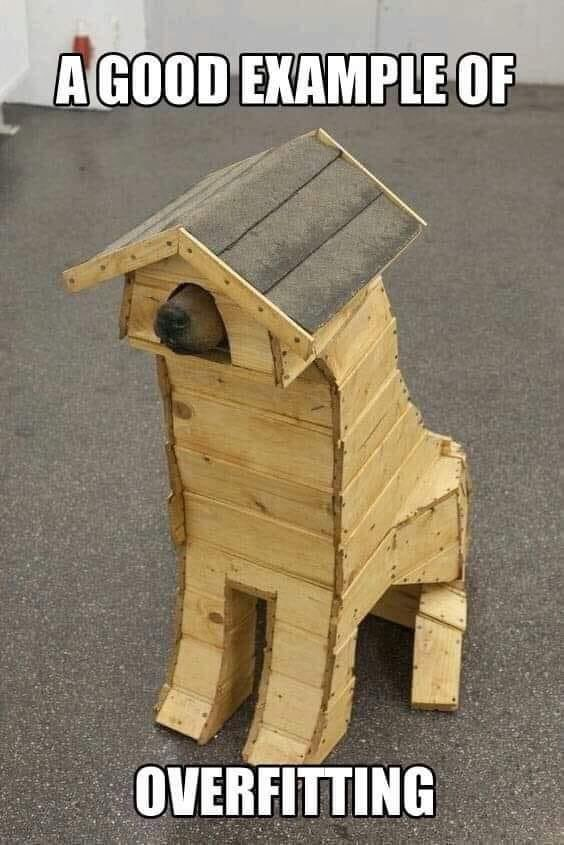
\includegraphics[width=\textwidth,height=2.08333in]{images/over1.jpg}
\caption{Overfitting: descripción gráfica}
\end{figure}

Lamentablemente la solución es una generalmente costosa y que no siempre tenemos a mano: incluir más casos etiquetados, con más variedad y vocabulario, y mejorar procesamientos e hiperparámetros.

\hypertarget{feature-engineering-modificar-datos}{%
\subsection{Feature engineering (modificar datos)}\label{feature-engineering-modificar-datos}}

Over y sub-sampling modifican la proporción de casos de la base de entrenamiento pero no modifican lo que los datos dicen en sí. Una estrategia alternativa es afinar o agregar \emph{más variables}, es decir, nuevas columnas que incluyan información adicional que el modelo pueda considerar. A estas tareas se les llama \emph{feature engineering} porque suponen ajustar/afinar las variables a considerar por el modelo.

Por ejemplo, con nuestra base podríamos:

\begin{itemize}
\tightlist
\item
  aumentar la cantidad de tokens o términos considerados, para dar cuenta de un vocabulario más amplio;
\item
  realizar un preprocesamiento distinto para las palabras;
\item
  incluir otras variables resultantes de algún cálculo, como por ejemplo, una rutina de \emph{sentiment analysis} que incluya una columna de score para cada oración. Esto últimos nos daría un enfoque híbrido para clasificar, posiblemente, con resultados mucho más robusto.
\end{itemize}

Vamos a probar esto último. Por simpleza, vamos a calcular un \emph{score} de sentimiento sobre la tabla \texttt{oraciones\_anotadas}, que tiene las oraciones anotadas por \texttt{udpipe}, de donde vamos a usar la función \texttt{txt\_sentiment}. Todo esto ya lo hicimos en un capítulo anterior, donde dijimos que el score dependía mayormente del largo de la oración, asi que vamos a normalizar ese valor dividiendo el score por la cantidad de términos.
Para poder considerar este valor lo vamos a agregar a nuestro objeto \texttt{or\_dtm2} (la matrix de términos por documentos) sobre la que estabamos trabajando.

\begin{Shaded}
\begin{Highlighting}[]
\NormalTok{lexicones }\OtherTok{\textless{}{-}}\NormalTok{ readr}\SpecialCharTok{::}\FunctionTok{read\_csv}\NormalTok{(}\StringTok{\textquotesingle{}https://raw.githubusercontent.com/gastonbecerra/curso{-}intro{-}r/main/data/lexicones.csv\textquotesingle{}}\NormalTok{)}
\end{Highlighting}
\end{Shaded}

\begin{verbatim}
## 
## -- Column specification -------------------------------------------------------------------------
## cols(
##   lemma = col_character(),
##   v = col_double()
## )
\end{verbatim}

\begin{Shaded}
\begin{Highlighting}[]
\CommentTok{\# preparamos el lexicon para que los términos tengan 2 valores: 1 positivas y {-}1 negativas}
\NormalTok{polarity\_terms }\OtherTok{\textless{}{-}}\NormalTok{ lexicones }\SpecialCharTok{\%\textgreater{}\%}
  \FunctionTok{mutate}\NormalTok{(}\AttributeTok{polarity =} \FunctionTok{if\_else}\NormalTok{(v}\SpecialCharTok{\textgreater{}}\DecValTok{0}\NormalTok{,}\DecValTok{1}\NormalTok{,}\SpecialCharTok{{-}}\DecValTok{1}\NormalTok{)) }\SpecialCharTok{\%\textgreater{}\%}
  \FunctionTok{select}\NormalTok{(}\AttributeTok{term=}\NormalTok{lemma, polarity)}

\CommentTok{\# preparamos los términos que modifican pesos}
\NormalTok{polarity\_negators }\OtherTok{\textless{}{-}} \FunctionTok{c}\NormalTok{(}\StringTok{"no"}\NormalTok{,}\StringTok{"nunca"}\NormalTok{,}\StringTok{"nadie"}\NormalTok{)}
\NormalTok{polarity\_amplifiers }\OtherTok{\textless{}{-}} \FunctionTok{c}\NormalTok{(}\StringTok{"muy"}\NormalTok{, }\StringTok{"mucho"}\NormalTok{, }\StringTok{"mas"}\NormalTok{)}
\NormalTok{polarity\_deamplifiers }\OtherTok{\textless{}{-}} \FunctionTok{c}\NormalTok{(}\StringTok{"poco"}\NormalTok{, }\StringTok{"casi"}\NormalTok{, }\StringTok{"alguno"}\NormalTok{, }\StringTok{"menos"}\NormalTok{)}

\CommentTok{\# corremos la función de sentiment analysis de udpipe}
\NormalTok{oraciones\_txt\_sentiment }\OtherTok{\textless{}{-}}\NormalTok{ udpipe}\SpecialCharTok{::}\FunctionTok{txt\_sentiment}\NormalTok{(}
  \AttributeTok{x =}\NormalTok{ oraciones\_anotadas,}
  \AttributeTok{term =} \StringTok{"lemma"}\NormalTok{,}
  \AttributeTok{polarity\_terms =}\NormalTok{ polarity\_terms,}
  \AttributeTok{polarity\_negators =}\NormalTok{ polarity\_negators,}
  \AttributeTok{polarity\_amplifiers =}\NormalTok{ polarity\_amplifiers,}
  \AttributeTok{polarity\_deamplifiers =}\NormalTok{ polarity\_deamplifiers)}\SpecialCharTok{$}\NormalTok{overall}

\CommentTok{\# chusmeemos el objeto}
\FunctionTok{glimpse}\NormalTok{(oraciones\_txt\_sentiment)}
\end{Highlighting}
\end{Shaded}

\begin{verbatim}
## Rows: 400
## Columns: 8
## $ doc_id              <chr> "3578", "2300", "405", "2540", "2016", "2713", "1503", "534", "1101~
## $ sentiment_polarity  <dbl> 10.0, 16.0, 8.0, 9.0, 4.0, 9.0, 8.0, 10.0, 7.0, 13.0, 10.0, 3.0, 11~
## $ sentences           <int> 1, 1, 1, 1, 1, 1, 1, 1, 1, 1, 1, 1, 1, 1, 1, 1, 1, 1, 1, 1, 1, 1, 1~
## $ terms               <int> 36, 37, 27, 21, 13, 25, 17, 30, 16, 35, 30, 9, 32, 16, 13, 17, 35, ~
## $ terms_positive      <chr> "almacenamiento, análisis, clasificación, describir, grande, inform~
## $ terms_negative      <chr> "dispositivo, que", "que", "que", "", "que", "que", "", "que", "", ~
## $ terms_negation      <chr> "", "", "", "", "", "", "", "", "", "", "", "", "", "", "", "", "",~
## $ terms_amplification <chr> "", "", "", "", "", "", "", "", "", "", "", "", "", "", "", "", "",~
\end{verbatim}

\begin{Shaded}
\begin{Highlighting}[]
\CommentTok{\# agregamos una columan en dtm con el score }
\NormalTok{or\_dtm2}\SpecialCharTok{$}\NormalTok{sentiment\_score }\OtherTok{=}\NormalTok{ (oraciones\_txt\_sentiment}\SpecialCharTok{$}\NormalTok{sentiment\_polarity }\SpecialCharTok{/}\NormalTok{ oraciones\_txt\_sentiment}\SpecialCharTok{$}\NormalTok{terms)}
\end{Highlighting}
\end{Shaded}

Ahora nuestra base incluye una variable más: \texttt{sentiment\_score}!
Pero metamos un chequeo rápido: grafiquemos este valor para cada registro, recordando que nuestra base tiene 300 registros positivos, seguidos de 100 negativos:

\begin{Shaded}
\begin{Highlighting}[]
\FunctionTok{plot}\NormalTok{(or\_dtm2}\SpecialCharTok{$}\NormalTok{sentiment\_score)}
\end{Highlighting}
\end{Shaded}

\includegraphics{curso-intro-r_files/figure-latex/unnamed-chunk-83-1.pdf}

Los resultados son mas o menos esperables con la división del dataset, no?

Vamos entonces a seguir con el camino que ya conocemos: vamos a hacer el split entre training y test (acá no necesitamos hacer la transformación que hicimos antes ya que \texttt{or\_dtm2} tiene la forma requerida por el algoritmo), y luego vamos a entrenar el modelo considerando esta nueva variable. Para esto vamos a usar la notación de función: \texttt{clase\_oracion\textasciitilde{}.+clase\_oracion}, donde indicamos que \texttt{clase\_oracion} es \emph{función de} \texttt{\textasciitilde{}.+clase\_oracion} = todas las otras variables y además \texttt{sentiment\_score}.

\begin{Shaded}
\begin{Highlighting}[]
\CommentTok{\# split entre training y test}
\FunctionTok{set.seed}\NormalTok{(}\DecValTok{100}\NormalTok{) }\CommentTok{\# seteamos una semilla, para poder reproducir los resultados}
\NormalTok{division }\OtherTok{=} \FunctionTok{sample.split}\NormalTok{(or\_dtm2}\SpecialCharTok{$}\NormalTok{clase\_oracion, }\AttributeTok{SplitRatio =} \FloatTok{0.7}\NormalTok{) }\CommentTok{\# divide 70/30}
\NormalTok{or\_train }\OtherTok{=} \FunctionTok{subset}\NormalTok{(or\_dtm2, division}\SpecialCharTok{==}\ConstantTok{TRUE}\NormalTok{) }\CommentTok{\# subconjunto de entrenamiento}
\NormalTok{or\_test }\OtherTok{=} \FunctionTok{subset}\NormalTok{(or\_dtm2, division}\SpecialCharTok{==}\ConstantTok{FALSE}\NormalTok{) }\CommentTok{\# subconjunto de testeo}

\CommentTok{\# vamos a convertir la variable con la etiqueta en factores}
\NormalTok{or\_train}\SpecialCharTok{$}\NormalTok{clase\_oracion }\OtherTok{=} \FunctionTok{as.factor}\NormalTok{(or\_train}\SpecialCharTok{$}\NormalTok{clase\_oracion)}
\NormalTok{or\_test}\SpecialCharTok{$}\NormalTok{clase\_oracion }\OtherTok{=} \FunctionTok{as.factor}\NormalTok{(or\_test}\SpecialCharTok{$}\NormalTok{clase\_oracion)}

\CommentTok{\# entrenamos modelo y predecimos}
\NormalTok{or\_rpart\_fe }\OtherTok{\textless{}{-}} \FunctionTok{rpart}\NormalTok{(clase\_oracion}\SpecialCharTok{\textasciitilde{}}\NormalTok{.}\SpecialCharTok{+}\NormalTok{sentiment\_score, }\AttributeTok{data =}\NormalTok{ or\_train, }\AttributeTok{method =} \StringTok{\textquotesingle{}class\textquotesingle{}}\NormalTok{) }\CommentTok{\# generamos el modelo}
\NormalTok{or\_rpart\_predict\_fe }\OtherTok{\textless{}{-}} \FunctionTok{predict}\NormalTok{(or\_rpart\_fe, or\_test, }\AttributeTok{type =} \StringTok{\textquotesingle{}class\textquotesingle{}}\NormalTok{) }\CommentTok{\# \# predecimos con tabla test, para evaluar contra real}

\FunctionTok{confusionMatrix}\NormalTok{(or\_test}\SpecialCharTok{$}\NormalTok{clase\_oracion, or\_rpart\_predict\_fe) }\CommentTok{\# veamos como nos fue}
\end{Highlighting}
\end{Shaded}

\begin{verbatim}
## Confusion Matrix and Statistics
## 
##           Reference
## Prediction negativo positivo
##   negativo       22        8
##   positivo        4       86
##                                           
##                Accuracy : 0.9             
##                  95% CI : (0.8318, 0.9473)
##     No Information Rate : 0.7833          
##     P-Value [Acc > NIR] : 0.0006378       
##                                           
##                   Kappa : 0.7209          
##                                           
##  Mcnemar's Test P-Value : 0.3864762       
##                                           
##             Sensitivity : 0.8462          
##             Specificity : 0.9149          
##          Pos Pred Value : 0.7333          
##          Neg Pred Value : 0.9556          
##              Prevalence : 0.2167          
##          Detection Rate : 0.1833          
##    Detection Prevalence : 0.2500          
##       Balanced Accuracy : 0.8805          
##                                           
##        'Positive' Class : negativo        
## 
\end{verbatim}

Mucho mejor! Notemos que con este enfoque ``hibrido'' no tuvimos que considerar nosotros cuál era el \emph{score} en el que una oración se volvía positiva o negativa.

\hypertarget{construcciuxf3n-de-datasets-borrador}{%
\chapter{Construcción de datasets (BORRADOR)}\label{construcciuxf3n-de-datasets-borrador}}

En este tutorial vamos a explorar distintas maneras de construir un dataset.

\begin{enumerate}
\def\labelenumi{\arabic{enumi}.}
\tightlist
\item
  Vamos a conectar con una API (Wikipedia) de la manera más básica;
\item
  Vamos a conectar con una API (Twitter) usando el paquete \texttt{rtweet};
\item
  Mencionamos las limtaciones de la API de Facebook;
\item
  Hacemos \emph{scrapping} para recuperar contenido de páginas web tipo OJS.
\end{enumerate}

Al final listamos algunos otros recursos donde se pueden obtener datasets.

\hypertarget{apis}{%
\section{APIs}\label{apis}}

Un API (Application Programming Interface) es una ``puerta de entrada'' que algunas aplicaciones ofrecen para interatuar con sus datos y sus funciones de forma ordenada.
Se puede utilizar una API para recuperar contenido de las bases de datos de la aplicación (e.g., obtener tweets de Twitter) de forma legal y dentro de las condiciones de acceso y uso que la aplicación impone.

Generalmente, las API se utilizan a través del protocolo HTTP, de modo que se puede interactuar con ella a través desde distintos lenguajes y/o programas que nos permita hacer \emph{requests} (acciones para leer, enviar y manipular datos) por internet, ya sea un navegador como Chrome, un programa específico como \href{https://learning.postman.com/}{Postman}, o R.

Cada API tiene su dirección URL, y una forma particular de requerir parámetros por medio de ella. Un ejemplo de un request simple que devuelve la información de una foto de Facebook es la siguiente URL, que se puede consultar desde el navegador: \url{https://graph.facebook.com/facebook/picture?redirect=false}.

El \emph{response} o resultado del request es sólo datos, es decir, contenido de la aplicación sin los elementos de diseño o interfaces.
Generalmente los datos se escriben en un formato flexible, como XML o JSON.
En ocasiones, hay algunos metadatos en los encabezados de las responses que indican cómo resultó nuestros request por medio de un código (e.g., un status 200 significa que el request se procesó OK, mientras un 404 indica que el recurso que buscamos no está disponible).

Muchas APIs requieren una autenticación para poder procesar un request, esto les permite regular el acceso a la información. Para ello, en algunos casos basta con proveer algunas credenciales que obtenemos al registrarnos como usuarios de la aplicación. En otros casos, como en las APIs de Facebook y Twitter, además es necesario registrarse como ``desarrollador'' y registrar una ``aplicación'' para la cual se piden ciertos permisos particulares, como leer o postear contenido. Como resultado de este registro generalmente obtenemos algunas ``llaves'' que incluimos en nuestros requests como parámetros. Otras APIs, como la de Google, tienen algunos servicios pagos y requieren que registremos una tarjeta de crédito en nuestro perfil, para cobrarnos por consumo.

Por suerte, para algunas aplicaciones contamos con paquetes de R para interactuar con sus APIs. Estos paquetes se encargan de formatear los request de pedido de información, incluyendo las claves de seguridad que hayamos obtenido, y/o leer los datos que nos devuelven en un formato compatible con R, como un dataframe.

\hypertarget{api-de-wikipedia-sin-paquetes}{%
\subsection{API de Wikipedia (Sin paquetes!)}\label{api-de-wikipedia-sin-paquetes}}

La primera API que vamos a explorar es la de Wikipedia.
Nos interesa esta API por 2 razones: (1) no requiere autenticación\ldots{} por lo menos para el tipo de request que vamos a estar haciendo;
y (2) no hay paquete de R para interactuar con ella, asi que vamos a usarla ``sin rueditas''\ldots. aunque vale la aclaración, si vamos a usar un paquete para hacer requests por HTTP, llamado \texttt{httr}.

Particularmente:

\begin{enumerate}
\def\labelenumi{\arabic{enumi}.}
\tightlist
\item
  vamos a hacer un request, componiendo una URL y llamandola por GET (un método del protocolo HTTP, que usás todo el tiempo para navegar);
\item
  vamos a leer el response, que está en formato JSON, y vamos a ver cómo lo podemos convertir a un formato más cómodo con R.
\end{enumerate}

Antes que nada, tenemos que saber qué clase de requests se pueden hacer (qué puedo preguntarle a la API). Todas las aplicaciones tienen una \emph{API Reference} que aclara esto; otras, mas copadas, tienen una \emph{API Explorer} que permite ``componer'' con formularios los parámetros de los requests y explorar los resultados. Wikipedia, por suerte es uno de ellos: \url{https://es.wikipedia.org/wiki/Especial:Zona_de_pruebas_de_la_API}.

Lo primero que vamos a hacer es buscar entradas que incluyan las palabras ``big data.''

Para hacer este request es necesario conocer como componer la URL. En el caso de Wikipedia esto se compone por una URL base (\texttt{https://es.wikipedia.org/w/api.php?}) seguido de la acción que nos interesa realizar: ``query'' porque vamos a buscar páginas (\texttt{\&action=query}).
Esta acción requiere un criterio (\texttt{\&srsearch=big\%20data}) y que especifiquemos qué devolver y en qué formato (\texttt{\&list=search\&format=json}):
\url{https://es.wikipedia.org/w/api.php?action=query\&list=search\&srsearch=big\%20data\&format=json}

\begin{Shaded}
\begin{Highlighting}[]
\FunctionTok{library}\NormalTok{(tidyverse)}

\NormalTok{criterio }\OtherTok{\textless{}{-}} \StringTok{"big\%20data"} \CommentTok{\# como es una URL hay que codificar algunos caracteres, como el espacio (\%20)}

\FunctionTok{library}\NormalTok{(httr) }\CommentTok{\# vamos usar este paquete para usar el protocolo HTTP}
\NormalTok{llamada }\OtherTok{\textless{}{-}}\NormalTok{ httr}\SpecialCharTok{::}\FunctionTok{GET}\NormalTok{(}\FunctionTok{paste0}\NormalTok{(}\StringTok{"https://es.wikipedia.org/w/api.php?action=query\&list=search\&format=json\&srsearch="}\NormalTok{, criterio)) }\CommentTok{\# hacemos el request via HTTP/GET}

\NormalTok{llamada}\SpecialCharTok{$}\NormalTok{status\_code }\CommentTok{\# si es 200, todo OK}
\end{Highlighting}
\end{Shaded}

\begin{verbatim}
## [1] 200
\end{verbatim}

Veamos un pedazo de la respuesta, que se encuentra en formato JSON:

\begin{verbatim}
{
  batchcomplete: "",
  continue: {
    sroffset: 10,
    continue: "-||"
  },
  query: {
    searchinfo: {
      totalhits: 6783
    },
    search: [
      {
        ns: 0,
        title: "Macrodatos",
        pageid: 5242736,
        size: 115077,
        wordcount: 13491,
        snippet: "también llamados datos masivos, inteligencia de datos, datos a gran escala o <span class="searchmatch">big</span> <span class="searchmatch">data</span> (terminología en idioma inglés utilizada comúnmente) es un término que",
        timestamp: "2021-06-03T16:23:33Z"
        },
      {
        ns: 0,
        title: "Big Bang",
        pageid: 6822,
        size: 71060,
        wordcount: 9270,
        snippet: "En cosmología, se entiende por <span class="searchmatch">Big</span> Bang,[1]​[2]​ también llamada la Gran Explosión (término proveniente del astrofísico Fred Hoyle a modo de burla de",
        timestamp: "2021-06-12T03:48:05Z"
        },
...
\end{verbatim}

Este contenido se puede acceder a través del \texttt{content} del objeto generado por \texttt{httr::GET}. Esta función convierte el JSON es una lista, es decir, una colección de objetos en R.

Esta lista tiene 4 elementos: \texttt{batchcomplete} y \texttt{continue} se usan para paginar los resultados; \texttt{query} que a su vez tiene 2 elementos: primero informa cuantos resultados hubo; y despues en \texttt{search} incluye los resultados. Arriba mostramos 2 resultados, que incluyen un título, un pageid, y otra info.

Veamos como podemos acceder a este JSON:

\begin{Shaded}
\begin{Highlighting}[]
\NormalTok{respuesta }\OtherTok{\textless{}{-}}\NormalTok{ httr}\SpecialCharTok{::}\FunctionTok{content}\NormalTok{(}\AttributeTok{x =}\NormalTok{ llamada) }\CommentTok{\# httr nos lee el content del objeto que generamos}

\FunctionTok{class}\NormalTok{(respuesta) }\CommentTok{\# chequeemos que es una lista}
\end{Highlighting}
\end{Shaded}

\begin{verbatim}
## [1] "list"
\end{verbatim}

\begin{Shaded}
\begin{Highlighting}[]
\FunctionTok{str}\NormalTok{(respuesta, }\AttributeTok{max=}\DecValTok{3}\NormalTok{) }\CommentTok{\# veamos su estructura ... lo que nos interesa está en query \textgreater{} search}
\end{Highlighting}
\end{Shaded}

\begin{verbatim}
## List of 3
##  $ batchcomplete: chr ""
##  $ continue     :List of 2
##   ..$ sroffset: int 10
##   ..$ continue: chr "-||"
##  $ query        :List of 2
##   ..$ searchinfo:List of 1
##   .. ..$ totalhits: int 6831
##   ..$ search    :List of 10
##   .. ..$ :List of 7
##   .. ..$ :List of 7
##   .. ..$ :List of 7
##   .. ..$ :List of 7
##   .. ..$ :List of 7
##   .. ..$ :List of 7
##   .. ..$ :List of 7
##   .. ..$ :List of 7
##   .. ..$ :List of 7
##   .. ..$ :List of 7
\end{verbatim}

\begin{Shaded}
\begin{Highlighting}[]
\NormalTok{resultados }\OtherTok{\textless{}{-}}\NormalTok{ respuesta[[}\StringTok{"query"}\NormalTok{]][[}\StringTok{"search"}\NormalTok{]] }\CommentTok{\# tomamos del objeto respuesta su objeto query, y luego su objeto "search"}
\end{Highlighting}
\end{Shaded}

La lista tiene dentro 1 lista por cada elemento (resultado). Como estas listas son iguales, podemos convertirlas a un formato tabla.

\begin{Shaded}
\begin{Highlighting}[]
\FunctionTok{library}\NormalTok{(dplyr) }\CommentTok{\# para transformar la lista vamos a usar dplyr}
\NormalTok{resultados\_df }\OtherTok{\textless{}{-}}\NormalTok{ dplyr}\SpecialCharTok{::}\FunctionTok{bind\_rows}\NormalTok{(resultados) }\CommentTok{\# vamos a separar las listas y unirlas en formato dataframe}
\FunctionTok{glimpse}\NormalTok{(resultados\_df) }\CommentTok{\# veamos la tabla armada}
\end{Highlighting}
\end{Shaded}

\begin{verbatim}
## Rows: 10
## Columns: 7
## $ ns        <int> 0, 0, 0, 0, 0, 0, 0, 0, 0, 0
## $ title     <chr> "Macrodatos", "Big Bang", "Tidy data", "Big Rapids", "Río Big Sioux", "Big Be~
## $ pageid    <int> 5242736, 6822, 8754307, 4702847, 2648540, 4102878, 4115045, 4103098, 480752, ~
## $ size      <int> 115077, 71060, 2054, 3911, 8016, 11851, 2731, 3073, 3007, 129354
## $ wordcount <int> 13491, 9270, 247, 319, 575, 1121, 208, 241, 494, 13781
## $ snippet   <chr> "también llamados datos masivos, inteligencia de datos, datos a gran escala o~
## $ timestamp <chr> "2021-06-03T16:23:33Z", "2021-06-12T03:48:05Z", "2020-08-26T21:03:30Z", "2019~
\end{verbatim}

Ahora vamos a usar estos valores para recuperar los contenidos de las páginas.

Para esta acción la URL base es la misma que veniamos usando (\texttt{https://es.wikipedia.org/w/api.php?}) seguido de la acción que nos interesa realizar: ``parse'' porque le pedimos que imprima una pagina (\texttt{\&action=parse}).
Esta acción requiere un criterio (\texttt{\&page=}) con el título que querramos recuperar, y finalmente, que especifiquemos qué en qué formatos (\texttt{\&list=search\&format=json}).

Veamos los títulos que podemos recuperar y compongamos la URL con los primeros.

\begin{Shaded}
\begin{Highlighting}[]
\NormalTok{resultados\_df}\SpecialCharTok{$}\NormalTok{title }\CommentTok{\# veamos cuales son los primeros titulos}
\end{Highlighting}
\end{Shaded}

\begin{verbatim}
##  [1] "Macrodatos"          "Big Bang"            "Tidy data"           "Big Rapids"         
##  [5] "Río Big Sioux"       "Big Bear Lake"       "Big Pine"            "Big Bear City"      
##  [9] "Big Water"           "The Big Bang Theory"
\end{verbatim}

\begin{Shaded}
\begin{Highlighting}[]
\NormalTok{criterio2 }\OtherTok{\textless{}{-}} \FunctionTok{str\_replace}\NormalTok{(}\AttributeTok{string =}\NormalTok{ resultados\_df}\SpecialCharTok{$}\NormalTok{title[}\DecValTok{1}\NormalTok{], }\AttributeTok{pattern =} \StringTok{" "}\NormalTok{, }\AttributeTok{replacement =} \StringTok{"\_"}\NormalTok{)  }\CommentTok{\# llamemos al primer elemento, reemplazando espacios por \_ .... esto hay que mejorarlo para encodear otros elementos, como acentos}

\FunctionTok{library}\NormalTok{(httr) }\CommentTok{\# vamos usar este paquete para usar el protocolo HTTP}
\NormalTok{llamada2 }\OtherTok{\textless{}{-}}\NormalTok{ httr}\SpecialCharTok{::}\FunctionTok{GET}\NormalTok{(}\FunctionTok{paste0}\NormalTok{(}\StringTok{"https://es.wikipedia.org/w/api.php?action=parse\&prop=text\&formatversion=2\&format=json\&page="}\NormalTok{, criterio2)) }\CommentTok{\# hacemos el request via HTTP/GET}

\NormalTok{llamada2}\SpecialCharTok{$}\NormalTok{status\_code }\CommentTok{\# veamos si devuelve 200 == OK}
\end{Highlighting}
\end{Shaded}

\begin{verbatim}
## [1] 200
\end{verbatim}

\begin{Shaded}
\begin{Highlighting}[]
\NormalTok{respuesta2 }\OtherTok{\textless{}{-}}\NormalTok{ httr}\SpecialCharTok{::}\FunctionTok{content}\NormalTok{(}\AttributeTok{x =}\NormalTok{ llamada2) }\CommentTok{\# httr nos lee el content del objeto que generamos}

\FunctionTok{class}\NormalTok{(respuesta2) }\CommentTok{\# chequeemos que es una lista}
\end{Highlighting}
\end{Shaded}

\begin{verbatim}
## [1] "list"
\end{verbatim}

\begin{Shaded}
\begin{Highlighting}[]
\FunctionTok{str}\NormalTok{(respuesta2, }\AttributeTok{max=}\DecValTok{3}\NormalTok{) }\CommentTok{\# veamos su estructura ... lo que nos interesa está en parse \textgreater{} text}
\end{Highlighting}
\end{Shaded}

\begin{verbatim}
## List of 1
##  $ parse:List of 3
##   ..$ title : chr "Macrodatos"
##   ..$ pageid: int 5242736
##   ..$ text  : chr "<div class=\"mw-parser-output\"><div class=\"thumb tright\"><div class=\"thumbinner\" style=\"width:252px;\"><a"| __truncated__
\end{verbatim}

\begin{Shaded}
\begin{Highlighting}[]
\NormalTok{respuesta2[[}\StringTok{"parse"}\NormalTok{]][[}\StringTok{"text"}\NormalTok{]] }\SpecialCharTok{\%\textgreater{}\%} \FunctionTok{str\_sub}\NormalTok{(}\AttributeTok{start =} \DecValTok{1}\NormalTok{, }\AttributeTok{end =} \DecValTok{500}\NormalTok{) }\CommentTok{\# tomemos un fragmento}
\end{Highlighting}
\end{Shaded}

\begin{verbatim}
## [1] "<div class=\"mw-parser-output\"><div class=\"thumb tright\"><div class=\"thumbinner\" style=\"width:252px;\"><a href=\"/wiki/Archivo:Viegas-UserActivityonWikipedia.gif\" class=\"image\"><img alt=\"\" src=\"//upload.wikimedia.org/wikipedia/commons/thumb/6/69/Viegas-UserActivityonWikipedia.gif/250px-Viegas-UserActivityonWikipedia.gif\" decoding=\"async\" width=\"250\" height=\"188\" class=\"thumbimage\" srcset=\"//upload.wikimedia.org/wikipedia/commons/thumb/6/69/Viegas-UserActivityonWikipedia.gif/375px-Viegas-UserActivit"
\end{verbatim}

Lo que vemos es el código fuente (HTML) de esta página: \url{https://es.wikipedia.org/wiki/Macrodatos}

\hypertarget{api-de-twitter-con-rtweet}{%
\subsection{API de Twitter (con rtweet)}\label{api-de-twitter-con-rtweet}}

Twitter requiere generar una \emph{aplicacion} y registrarla en una \emph{cuenta de desarrollador}. Para es necesario:

\begin{enumerate}
\def\labelenumi{\arabic{enumi}.}
\tightlist
\item
  Registrarse en \href{https://developer.twitter.com/en}{Twitter developers} y aplicar al acceso: \url{https://developer.twitter.com/en/apply-for-access}
\item
  Crear un \emph{proyecto}: \url{https://developer.twitter.com/en/portal/projects/new}
\end{enumerate}

Para esto te va a pedir que definas: tipo de proyecto (academico), descripcion (objetivos, posta), crear/vincularla a una app (va a pedir solo el nombre). Twitter aclara: \emph{Apps are where you get your access keys and tokens and set permissions}.

Luego, vamos a ir a la pagina de app que acabamos de crear, a buscar las credenciales para acceder:

(Estamos usando el metodo de generar un \emph{token}\ldots{} pero hay otros: \url{https://cran.r-project.org/web/packages/rtweet/vignettes/auth.html})

\begin{enumerate}
\def\labelenumi{\arabic{enumi}.}
\setcounter{enumi}{2}
\tightlist
\item
  Vamos a configurar las app permissions, que habilitan a distintas acciones, como buscar y leer tweets, o postear.
\item
  Vasmo a configurar credenciales, yendo a ``Keys and tokens''
\end{enumerate}

Aquí vamos a buscar ``API Key and Secret'' y ``Access Token and Secret.'' Ambos tienen 2 claves: key y secret key.

\begin{Shaded}
\begin{Highlighting}[]
\CommentTok{\# estos datos son de ejemplo...}

\NormalTok{api\_key }\OtherTok{\textless{}{-}} \StringTok{"afYS4vbIlPAj096E60c4W1fiK"}
\NormalTok{api\_secret\_key }\OtherTok{\textless{}{-}} \StringTok{"bI91kqnqFoNCrZFbsjAWHD4gJ91LQAhdCJXCj3yscfuULtNkuu"}
\NormalTok{access\_token }\OtherTok{\textless{}{-}} \StringTok{"9551451262{-}wK2EmA942kxZYIwa5LMKZoQA4Xc2uyIiEwu2YXL"}
\NormalTok{access\_token\_secret }\OtherTok{\textless{}{-}} \StringTok{"9vpiSGKg1fIPQtxc5d5ESiFlZQpfbknEN1f1m2xe5byw7"}
\end{Highlighting}
\end{Shaded}

Con estas 4 claves mas el nombre de la app, ya podemos ir al codigo, a trabajar con el paquete \texttt{rtweet}. Vamos a registrar un \emph{token} que queda en memoria y que el pack va a usar para autenticar cada pedido a twitter.

\begin{Shaded}
\begin{Highlighting}[]
\FunctionTok{library}\NormalTok{(rtweet)}
\end{Highlighting}
\end{Shaded}

\begin{verbatim}
## 
## Attaching package: 'rtweet'
\end{verbatim}

\begin{verbatim}
## The following object is masked from 'package:purrr':
## 
##     flatten
\end{verbatim}

\begin{Shaded}
\begin{Highlighting}[]
\NormalTok{token }\OtherTok{\textless{}{-}} \FunctionTok{create\_token}\NormalTok{(}
  \AttributeTok{app =}\NormalTok{ registered\_app,}
  \AttributeTok{consumer\_key =}\NormalTok{ api\_key,}
  \AttributeTok{consumer\_secret =}\NormalTok{ api\_secret\_key,}
  \AttributeTok{access\_token =}\NormalTok{ access\_token,}
  \AttributeTok{access\_secret =}\NormalTok{ access\_token\_secret) }\CommentTok{\# creamos token de autenticacion en memoria}
\end{Highlighting}
\end{Shaded}

Ahora ya estamos en condiciones de buscar tweets.

\begin{Shaded}
\begin{Highlighting}[]
\FunctionTok{library}\NormalTok{(tidyverse)}
\NormalTok{tweets }\OtherTok{\textless{}{-}} \FunctionTok{search\_tweets}\NormalTok{(}\AttributeTok{q =} \StringTok{"\#bigdata"}\NormalTok{,}\AttributeTok{n =} \DecValTok{20}\NormalTok{,}\AttributeTok{lang =} \StringTok{"es"}\NormalTok{, }\AttributeTok{include\_rts =} \ConstantTok{FALSE}\NormalTok{)}

\FunctionTok{names}\NormalTok{(tweets)}
\end{Highlighting}
\end{Shaded}

\begin{verbatim}
##  [1] "user_id"                 "status_id"               "created_at"             
##  [4] "screen_name"             "text"                    "source"                 
##  [7] "display_text_width"      "reply_to_status_id"      "reply_to_user_id"       
## [10] "reply_to_screen_name"    "is_quote"                "is_retweet"             
## [13] "favorite_count"          "retweet_count"           "quote_count"            
## [16] "reply_count"             "hashtags"                "symbols"                
## [19] "urls_url"                "urls_t.co"               "urls_expanded_url"      
## [22] "media_url"               "media_t.co"              "media_expanded_url"     
## [25] "media_type"              "ext_media_url"           "ext_media_t.co"         
## [28] "ext_media_expanded_url"  "ext_media_type"          "mentions_user_id"       
## [31] "mentions_screen_name"    "lang"                    "quoted_status_id"       
## [34] "quoted_text"             "quoted_created_at"       "quoted_source"          
## [37] "quoted_favorite_count"   "quoted_retweet_count"    "quoted_user_id"         
## [40] "quoted_screen_name"      "quoted_name"             "quoted_followers_count" 
## [43] "quoted_friends_count"    "quoted_statuses_count"   "quoted_location"        
## [46] "quoted_description"      "quoted_verified"         "retweet_status_id"      
## [49] "retweet_text"            "retweet_created_at"      "retweet_source"         
## [52] "retweet_favorite_count"  "retweet_retweet_count"   "retweet_user_id"        
## [55] "retweet_screen_name"     "retweet_name"            "retweet_followers_count"
## [58] "retweet_friends_count"   "retweet_statuses_count"  "retweet_location"       
## [61] "retweet_description"     "retweet_verified"        "place_url"              
## [64] "place_name"              "place_full_name"         "place_type"             
## [67] "country"                 "country_code"            "geo_coords"             
## [70] "coords_coords"           "bbox_coords"             "status_url"             
## [73] "name"                    "location"                "description"            
## [76] "url"                     "protected"               "followers_count"        
## [79] "friends_count"           "listed_count"            "statuses_count"         
## [82] "favourites_count"        "account_created_at"      "verified"               
## [85] "profile_url"             "profile_expanded_url"    "account_lang"           
## [88] "profile_banner_url"      "profile_background_url"  "profile_image_url"
\end{verbatim}

\begin{Shaded}
\begin{Highlighting}[]
\FunctionTok{glimpse}\NormalTok{(tweets)}
\end{Highlighting}
\end{Shaded}

\begin{verbatim}
## Rows: 20
## Columns: 90
## $ user_id                 <chr> "872131876168900608", "994948727566753792", "122716346017531084~
## $ status_id               <chr> "1404493839579107328", "1404493587845427202", "1404490451143606~
## $ created_at              <dttm> 2021-06-14 17:40:00, 2021-06-14 17:39:00, 2021-06-14 17:26:32,~
## $ screen_name             <chr> "ECON_Automation", "citicven", "MariaGuzur", "GrupoAIS", "con10~
## $ text                    <chr> "Smart Management System (SMS), otro de nuestros productos #Sma~
## $ source                  <chr> "Twitter Web App", "TweetDeck", "Twitter Web App", "Twitter Web~
## $ display_text_width      <dbl> 254, 171, 277, 268, 272, 254, 262, 278, 262, 275, 267, 209, 276~
## $ reply_to_status_id      <chr> NA, NA, NA, NA, "1404470968593141766", NA, NA, NA, NA, NA, NA, ~
## $ reply_to_user_id        <chr> NA, NA, NA, NA, "1668435678", NA, NA, NA, NA, NA, NA, NA, NA, N~
## $ reply_to_screen_name    <chr> NA, NA, NA, NA, "MedicoFernandez", NA, NA, NA, NA, NA, NA, NA, ~
## $ is_quote                <lgl> FALSE, FALSE, FALSE, FALSE, FALSE, FALSE, FALSE, FALSE, FALSE, ~
## $ is_retweet              <lgl> FALSE, FALSE, FALSE, FALSE, FALSE, FALSE, FALSE, FALSE, FALSE, ~
## $ favorite_count          <int> 0, 0, 1, 0, 0, 2, 0, 0, 0, 0, 0, 0, 0, 0, 0, 1, 0, 1, 1, 0
## $ retweet_count           <int> 0, 1, 1, 0, 0, 1, 0, 1, 0, 1, 0, 0, 1, 0, 0, 0, 0, 0, 0, 0
## $ quote_count             <int> NA, NA, NA, NA, NA, NA, NA, NA, NA, NA, NA, NA, NA, NA, NA, NA,~
## $ reply_count             <int> NA, NA, NA, NA, NA, NA, NA, NA, NA, NA, NA, NA, NA, NA, NA, NA,~
## $ hashtags                <list> <"SmartFactory", "Automation", "Manufacturing", "BigData", "IoT~
## $ symbols                 <list> NA, NA, NA, NA, NA, NA, NA, NA, NA, NA, NA, NA, NA, NA, NA, NA,~
## $ urls_url                <list> "econ-tech.com/wp-content/upl…", "citicven.la", "gzmaria97.wix~
## $ urls_t.co               <list> "https://t.co/uD4UE15vJw", "https://t.co/b6pJ7XUD2L", "https:/~
## $ urls_expanded_url       <list> "https://econ-tech.com/wp-content/uploads/2020/06/Caso-de-Exit~
## $ media_url               <list> "http://pbs.twimg.com/media/E3vLN9pWQAEX5MQ.png", "http://pbs.~
## $ media_t.co              <list> "https://t.co/Nz52uQM5wE", "https://t.co/URmJQuK8h4", NA, "htt~
## $ media_expanded_url      <list> "https://twitter.com/ECON_Automation/status/140449383957910732~
## $ media_type              <list> "photo", "photo", NA, "photo", NA, "photo", "photo", NA, "phot~
## $ ext_media_url           <list> "http://pbs.twimg.com/media/E3vLN9pWQAEX5MQ.png", "http://pbs.~
## $ ext_media_t.co          <list> "https://t.co/Nz52uQM5wE", "https://t.co/URmJQuK8h4", NA, "htt~
## $ ext_media_expanded_url  <list> "https://twitter.com/ECON_Automation/status/140449383957910732~
## $ ext_media_type          <chr> NA, NA, NA, NA, NA, NA, NA, NA, NA, NA, NA, NA, NA, NA, NA, NA~
## $ mentions_user_id        <list> NA, <"3017145715", "994948727566753792">, NA, <"171962485", "1~
## $ mentions_screen_name    <list> NA, <"QualitasGlobal", "citicven">, NA, <"Leandrosoft", "Felaba~
## $ lang                    <chr> "es", "es", "es", "es", "es", "es", "es", "es", "es", "es", "e~
## $ quoted_status_id        <chr> NA, NA, NA, NA, NA, NA, NA, NA, NA, NA, NA, NA, NA, NA, NA, "1~
## $ quoted_text             <chr> NA, NA, NA, NA, NA, NA, NA, NA, NA, NA, NA, NA, NA, NA, NA, "¡A~
## $ quoted_created_at       <dttm> NA, NA, NA, NA, NA, NA, NA, NA, NA, NA, NA, NA, NA, NA, NA, 202~
## $ quoted_source           <chr> NA, NA, NA, NA, NA, NA, NA, NA, NA, NA, NA, NA, NA, NA, NA, "Tw~
## $ quoted_favorite_count   <int> NA, NA, NA, NA, NA, NA, NA, NA, NA, NA, NA, NA, NA, NA, NA, 2,~
## $ quoted_retweet_count    <int> NA, NA, NA, NA, NA, NA, NA, NA, NA, NA, NA, NA, NA, NA, NA, 1, ~
## $ quoted_user_id          <chr> NA, NA, NA, NA, NA, NA, NA, NA, NA, NA, NA, NA, NA, NA, NA, "19~
## $ quoted_screen_name      <chr> NA, NA, NA, NA, NA, NA, NA, NA, NA, NA, NA, NA, NA, NA, NA, "mi~
## $ quoted_name             <chr> NA, NA, NA, NA, NA, NA, NA, NA, NA, NA, NA, NA, NA, NA, NA, "Mi~
## $ quoted_followers_count  <int> NA, NA, NA, NA, NA, NA, NA, NA, NA, NA, NA, NA, NA, NA, NA, 124~
## $ quoted_friends_count    <int> NA, NA, NA, NA, NA, NA, NA, NA, NA, NA, NA, NA, NA, NA, NA, 309~
## $ quoted_statuses_count   <int> NA, NA, NA, NA, NA, NA, NA, NA, NA, NA, NA, NA, NA, NA, NA, 691~
## $ quoted_location         <chr> NA, NA, NA, NA, NA, NA, NA, NA, NA, NA, NA, NA, NA, NA, NA, "Sp~
## $ quoted_description      <chr> NA, NA, NA, NA, NA, NA, NA, NA, NA, NA, NA, NA, NA, NA, NA, "Mi~
## $ quoted_verified         <lgl> NA, NA, NA, NA, NA, NA, NA, NA, NA, NA, NA, NA, NA, NA, NA, FAL~
## $ retweet_status_id       <chr> NA, NA, NA, NA, NA, NA, NA, NA, NA, NA, NA, NA, NA, NA, NA, NA,~
## $ retweet_text            <chr> NA, NA, NA, NA, NA, NA, NA, NA, NA, NA, NA, NA, NA, NA, NA, NA,~
## $ retweet_created_at      <dttm> NA, NA, NA, NA, NA, NA, NA, NA, NA, NA, NA, NA, NA, NA, NA, NA,~
## $ retweet_source          <chr> NA, NA, NA, NA, NA, NA, NA, NA, NA, NA, NA, NA, NA, NA, NA, NA,~
## $ retweet_favorite_count  <int> NA, NA, NA, NA, NA, NA, NA, NA, NA, NA, NA, NA, NA, NA, NA, NA~
## $ retweet_retweet_count   <int> NA, NA, NA, NA, NA, NA, NA, NA, NA, NA, NA, NA, NA, NA, NA, NA,~
## $ retweet_user_id         <chr> NA, NA, NA, NA, NA, NA, NA, NA, NA, NA, NA, NA, NA, NA, NA, NA,~
## $ retweet_screen_name     <chr> NA, NA, NA, NA, NA, NA, NA, NA, NA, NA, NA, NA, NA, NA, NA, NA,~
## $ retweet_name            <chr> NA, NA, NA, NA, NA, NA, NA, NA, NA, NA, NA, NA, NA, NA, NA, NA,~
## $ retweet_followers_count <int> NA, NA, NA, NA, NA, NA, NA, NA, NA, NA, NA, NA, NA, NA, NA, NA,~
## $ retweet_friends_count   <int> NA, NA, NA, NA, NA, NA, NA, NA, NA, NA, NA, NA, NA, NA, NA, NA,~
## $ retweet_statuses_count  <int> NA, NA, NA, NA, NA, NA, NA, NA, NA, NA, NA, NA, NA, NA, NA, NA,~
## $ retweet_location        <chr> NA, NA, NA, NA, NA, NA, NA, NA, NA, NA, NA, NA, NA, NA, NA, NA,~
## $ retweet_description     <chr> NA, NA, NA, NA, NA, NA, NA, NA, NA, NA, NA, NA, NA, NA, NA, NA,~
## $ retweet_verified        <lgl> NA, NA, NA, NA, NA, NA, NA, NA, NA, NA, NA, NA, NA, NA, NA, NA,~
## $ place_url               <chr> NA, NA, NA, NA, NA, NA, NA, NA, NA, NA, NA, NA, NA, NA, NA, NA,~
## $ place_name              <chr> NA, NA, NA, NA, NA, NA, NA, NA, NA, NA, NA, NA, NA, NA, NA, NA,~
## $ place_full_name         <chr> NA, NA, NA, NA, NA, NA, NA, NA, NA, NA, NA, NA, NA, NA, NA, NA,~
## $ place_type              <chr> NA, NA, NA, NA, NA, NA, NA, NA, NA, NA, NA, NA, NA, NA, NA, NA,~
## $ country                 <chr> NA, NA, NA, NA, NA, NA, NA, NA, NA, NA, NA, NA, NA, NA, NA, NA,~
## $ country_code            <chr> NA, NA, NA, NA, NA, NA, NA, NA, NA, NA, NA, NA, NA, NA, NA, NA,~
## $ geo_coords              <list> <NA, NA>, <NA, NA>, <NA, NA>, <NA, NA>, <NA, NA>, <NA, NA>, <NA~
## $ coords_coords           <list> <NA, NA>, <NA, NA>, <NA, NA>, <NA, NA>, <NA, NA>, <NA, NA>, <NA~
## $ bbox_coords             <list> <NA, NA, NA, NA, NA, NA, NA, NA>, <NA, NA, NA, NA, NA, NA, NA,~
## $ status_url              <chr> "https://twitter.com/ECON_Automation/status/140449383957910732~
## $ name                    <chr> "ECON Tech", "CiTICven", "María Gutiérrez", "AIS", "Opino en d~
## $ location                <chr> "Puebla, México", "Caracas, Venezuela", "VIT/VLL/SEV", "Barcelo~
## $ description             <chr> "Somos expertos en tecnología avanzada para control de procesos~
## $ url                     <chr> "https://t.co/rESTisWvVv", "https://t.co/txqe2OZ3J8", "https://~
## $ protected               <lgl> FALSE, FALSE, FALSE, FALSE, FALSE, FALSE, FALSE, FALSE, FALSE, ~
## $ followers_count         <int> 454, 251, 30, 373, 140, 3686, 155, 1099, 370, 2647, 386, 649, 6~
## $ friends_count           <int> 318, 196, 92, 124, 752, 1292, 664, 3373, 479, 567, 955, 490, 77~
## $ listed_count            <int> 11, 4, 0, 41, 1, 120, 1, 150, 7, 69, 0, 65, 0, 682, 1105, 391, ~
## $ statuses_count          <int> 7569, 1766, 72, 2102, 2757, 5582, 163, 2824, 1899, 8468, 2299, ~
## $ favourites_count        <int> 131, 127, 6, 804, 2010, 3603, 249, 567, 184, 1199, 323, 3408, 6~
## $ account_created_at      <dttm> 2017-06-06 16:43:37, 2018-05-11 14:33:56, 2020-02-11 09:32:34, ~
## $ verified                <lgl> FALSE, FALSE, FALSE, FALSE, FALSE, FALSE, FALSE, FALSE, FALSE, ~
## $ profile_url             <chr> "https://t.co/rESTisWvVv", "https://t.co/txqe2OZ3J8", "https:/~
## $ profile_expanded_url    <chr> "http://www.econ-tech.com", "http://citicven.la", "https://gzma~
## $ account_lang            <lgl> NA, NA, NA, NA, NA, NA, NA, NA, NA, NA, NA, NA, NA, NA, NA, NA,~
## $ profile_banner_url      <chr> "https://pbs.twimg.com/profile_banners/872131876168900608/16221~
## $ profile_background_url  <chr> "http://abs.twimg.com/images/themes/theme1/bg.png", NA, NA, "ht~
## $ profile_image_url       <chr> "http://pbs.twimg.com/profile_images/1322742634335657984/TsQBYG~
\end{verbatim}

Además de buscar tweets hay otras funciones:

\begin{Shaded}
\begin{Highlighting}[]
\NormalTok{?rtweet}\SpecialCharTok{::}\FunctionTok{search\_users}\NormalTok{() }\CommentTok{\# busca usuarios}
\NormalTok{?rtweet}\SpecialCharTok{::}\FunctionTok{get\_trends}\NormalTok{()  }\CommentTok{\# busca tendencias en algún lugar (por latitud y longitud)}
\NormalTok{?rtweet}\SpecialCharTok{::}\FunctionTok{get\_timeline}\NormalTok{() }\CommentTok{\# busca los tweets de 1 o mas usuarios}
\end{Highlighting}
\end{Shaded}

Sobre los límites del API de Twitter: \url{https://developer.twitter.com/en/docs/twitter-api/v1/rate-limits}

\hypertarget{una-nota-sobre-la-api-de-facebook}{%
\subsection{Una nota sobre la API de Facebook}\label{una-nota-sobre-la-api-de-facebook}}

Facebook impuso serias limitaciones a la información que es posible consultar via API.

Al igual que Twitter, Facebook requiere registrar una app. Pero, los tipos de apps que se sugieren y los permisos a otorgar, son indicativos del poco acceso que se puede obtener a los contenidos de la red social para investigación, dejando la API mayormente para interactuar y controlar campañas y negocios: \url{https://developers.facebook.com/docs/development/create-an-app/app-dashboard/app-types}.

Lo más cercano que hay al \emph{feed} de contenido social publicado por los usuarios, se limita a las páginas de las empresas, para lo que hay que tener una cuenta de negocios asociada a la página, y además someterse a una revisión de la app. \url{https://developers.facebook.com/docs/permissions/reference/pages_read_user_content/}

En contrapartida, Facebook ofrece algunos datasets: \url{https://research.fb.com/data/}

Mas info: \url{https://theconversation.com/facebooks-data-lockdown-is-a-disaster-for-academic-researchers-94533}

Como resultado de estos cambios, uno de los paquetes más usados para interactuar con el API de Facebook para R (\url{https://github.com/pablobarbera/Rfacebook}) ya no se mantiene más\ldots{}

\hypertarget{web-scraping}{%
\section{Web Scraping}\label{web-scraping}}

El proceso de recuperar contenido de manera automática a partir de páginas web se conoce como \emph{Web Scraping}.

Para poder recuperar contenido de páginas web hay \emph{2 requisitos}: tenemos que averiguar:

\begin{enumerate}
\def\labelenumi{\arabic{enumi}.}
\tightlist
\item
  las URLs de las páginas que queremos leer: en muchos casos pueden ser URLs dinámicas, con parámetros y valores, que podemos manipular.
\item
  la estructura HTML de la página donde está el contenido: como probablemente no nos interese \emph{todo el contenido de la página} (logos,textos,botones) sino sólo algunos textos, tenemos que poder identificar en qué parte del template de la página se insertan los contenidos que nos interesa, para así poder mapearlos.
\end{enumerate}

Ambas informaciones varían de sitio en sitio y de sistema en sistema. Para lo primero conviene entender lo básico de la sintáxis de las URLs: \url{https://en.wikipedia.org/wiki/URL\#Syntax}; para lo segundo, comprender lo básico de HTML markup \url{https://en.wikipedia.org/wiki/HTML\#Markup}, incluyendo como tomar los identificadores de un pedazo de sitio \url{https://towardsdatascience.com/web-scraping-in-r-using-rvest-and-selectorgadget-5fc5124547e}, algo para lo que el Dev.Tools del Chrome (F12 navegando la página) puede ser muy util.

\hypertarget{webscraping-resultados-de-buxfaqsqueda-de-ojs}{%
\subsection{Webscraping resultados de búqsqueda de OJS}\label{webscraping-resultados-de-buxfaqsqueda-de-ojs}}

Open Journal Systems (OJS) es un sistema de manejo editorial para revistas académicas. Es usado mayormente por universidades y por revistas que no tienen acuerdos editoriales con grandes empresas.

En este tutorial vamos a intentar recuperar los links a los artículos sobre ``big data'' que estén publicados en un listado de revistas que utilizan el sistema OJS:

\begin{Shaded}
\begin{Highlighting}[]
\NormalTok{sitios\_ojs }\OtherTok{=} \FunctionTok{c}\NormalTok{(}
  \StringTok{"http://ojs.sociologia{-}alas.org/index.php/CyC/"}\NormalTok{,}
  \StringTok{"http://ediciones.ucsh.cl/ojs/index.php/TSUCSH/"}\NormalTok{,}
  \CommentTok{\#"https://revistachasqui.org/index.php/chasqui/", \# tiene muchos resultados}
  \StringTok{"http://revistamexicanadesociologia.unam.mx/index.php/rms/"}
\NormalTok{  )}
\end{Highlighting}
\end{Shaded}

Nuestro \textbf{primer requisito} es averiguar las URLs de las páginas que queremos leer.

Recordemos que queremos encontrar sólo artículos que contengan ``big data,'' de modo que necesitamos utilizar la función de búsqueda de cada OJS. Luego de realizar algunas búsqueda ``a mano'' y obsevar cómo el OJS construye sus URLs (\url{https://docs.pkp.sfu.ca/dev/documentation/en/architecture-routes}), podemos armar las de los resultados de búsqueda:

\begin{Shaded}
\begin{Highlighting}[]
\NormalTok{criterio }\OtherTok{\textless{}{-}} \StringTok{"\%22big+data\%22"}
\NormalTok{url\_scrapear }\OtherTok{\textless{}{-}} \FunctionTok{paste}\NormalTok{( sitios\_ojs , }\CommentTok{\# vamos a contatenar pedazos de textos}
                       \StringTok{"search/search?query="}\NormalTok{,}
\NormalTok{                       criterio,}
                       \AttributeTok{sep =} \StringTok{""}\NormalTok{)}
\NormalTok{url\_scrapear}
\end{Highlighting}
\end{Shaded}

\begin{verbatim}
## [1] "http://ojs.sociologia-alas.org/index.php/CyC/search/search?query=%22big+data%22"            
## [2] "http://ediciones.ucsh.cl/ojs/index.php/TSUCSH/search/search?query=%22big+data%22"           
## [3] "http://revistamexicanadesociologia.unam.mx/index.php/rms/search/search?query=%22big+data%22"
\end{verbatim}

Ya tenemos listo el primer requisito: las URLs de las páginas a leer!

Nuestro \textbf{segundo requisito} es encontrar algún patrón para identificar el pedazo de contenido que nos interesa. En nuestro caso, se trata de los links a los artículos, de modo que, otra vez, tenemos que ver cómo se componen las URLs del OJS. Según su convención, los artículos en OJS tienen una URL con esta estructura: url\_sitio + ``/article/view/'' + id\_artículo. Con XPath, podemos escribir una expresión que filtre este tipo de link: \texttt{//a{[}contains(@href,\ "/article/view/"){]}}.

Ya tenemos listo el primer requisito: el patrón para identificar el contenido!

Ahora vamos a podemos comenzar con el scraping. Aquí vamos a ayudarnos con el paquete \texttt{rvest}.

\begin{Shaded}
\begin{Highlighting}[]
\FunctionTok{library}\NormalTok{(rvest)}

\NormalTok{tomar\_links\_resultados }\OtherTok{\textless{}{-}} \ControlFlowTok{function}\NormalTok{( url ) \{}
\NormalTok{  url\_con }\OtherTok{\textless{}{-}} \FunctionTok{url}\NormalTok{(url, }\StringTok{"rb"}\NormalTok{) }\CommentTok{\# abrimos una conexion para leer la pagina}
\NormalTok{  webpage }\OtherTok{\textless{}{-}}\NormalTok{ xml2}\SpecialCharTok{::}\FunctionTok{read\_html}\NormalTok{(url\_con) }\CommentTok{\# leemos la pagina}
  \FunctionTok{close}\NormalTok{(url\_con) }\CommentTok{\# cerramos la conexion}
\NormalTok{  xpath }\OtherTok{\textless{}{-}} \StringTok{\textquotesingle{}//a[contains(@href, "/article/view/")]\textquotesingle{}} \CommentTok{\# XPath para distinguir links a artículos}
\NormalTok{  links }\OtherTok{\textless{}{-}}\NormalTok{ rvest}\SpecialCharTok{::}\FunctionTok{html\_nodes}\NormalTok{(webpage, }\AttributeTok{xpath =}\NormalTok{ xpath) }\SpecialCharTok{\%\textgreater{}\%} \CommentTok{\# leemos los pedazos de codigo de links}
    \FunctionTok{html\_attr}\NormalTok{(}\StringTok{\textquotesingle{}href\textquotesingle{}}\NormalTok{) }\SpecialCharTok{\%\textgreater{}\%} \CommentTok{\# nos quedamos solo con la URL de los links}
    \FunctionTok{return}\NormalTok{()}
\NormalTok{\}}

\NormalTok{links\_articulos }\OtherTok{\textless{}{-}} \FunctionTok{character}\NormalTok{()}

\ControlFlowTok{for}\NormalTok{ (i }\ControlFlowTok{in} \DecValTok{1}\SpecialCharTok{:}\FunctionTok{length}\NormalTok{(url\_scrapear)) \{ }\CommentTok{\# vamos a ejecutar un bucle, donde i toma el valor del indice del array de URLs a visitar}
  \FunctionTok{message}\NormalTok{(}\StringTok{"scrapeando "}\NormalTok{,url\_scrapear[i]) }\CommentTok{\# que nos muestre en pantalla por donde anda}
\NormalTok{  links\_articulos }\OtherTok{\textless{}{-}} \FunctionTok{c}\NormalTok{(links\_articulos, }\FunctionTok{tomar\_links\_resultados}\NormalTok{(url\_scrapear[i]))}
\NormalTok{\}}
\end{Highlighting}
\end{Shaded}

\begin{verbatim}
## scrapeando http://ojs.sociologia-alas.org/index.php/CyC/search/search?query=%22big+data%22
\end{verbatim}

\begin{verbatim}
## scrapeando http://ediciones.ucsh.cl/ojs/index.php/TSUCSH/search/search?query=%22big+data%22
\end{verbatim}

\begin{verbatim}
## scrapeando http://revistamexicanadesociologia.unam.mx/index.php/rms/search/search?query=%22big+data%22
\end{verbatim}

\begin{Shaded}
\begin{Highlighting}[]
\NormalTok{links\_articulos}
\end{Highlighting}
\end{Shaded}

\begin{verbatim}
## [1] "http://ojs.sociologia-alas.org/index.php/CyC/article/view/245"                    
## [2] "http://ojs.sociologia-alas.org/index.php/CyC/article/view/219"                    
## [3] "http://ojs.sociologia-alas.org/index.php/CyC/article/view/213"                    
## [4] "http://ojs.sociologia-alas.org/index.php/CyC/article/view/151"                    
## [5] "http://ojs.sociologia-alas.org/index.php/CyC/article/view/131"                    
## [6] "http://ediciones.ucsh.cl/ojs/index.php/TSUCSH/article/view/268"                   
## [7] "http://revistamexicanadesociologia.unam.mx/index.php/rms/article/view/57723"      
## [8] "http://revistamexicanadesociologia.unam.mx/index.php/rms/article/view/57723/51185"
\end{verbatim}

Listo, tenemos los links de los artículos donde dice ``big data'' en varias revistas distintas. Ahora, seguro nos interese hacer un nuevo proceso de scraping para recuperar algunos metadatos de esos artículos. Pero para eso, mejor usemos el paquete \texttt{ojsr}.

\begin{Shaded}
\begin{Highlighting}[]
\FunctionTok{library}\NormalTok{(ojsr)}

\NormalTok{metadata }\OtherTok{\textless{}{-}}\NormalTok{ ojsr}\SpecialCharTok{::}\FunctionTok{get\_html\_meta\_from\_article}\NormalTok{(}\AttributeTok{input\_url =}\NormalTok{ links\_articulos, }\AttributeTok{verbose =} \ConstantTok{TRUE}\NormalTok{)}
\end{Highlighting}
\end{Shaded}

\begin{verbatim}
## trying url 1/8 http://ojs.sociologia-alas.org/index.php/CyC/article/view/245
\end{verbatim}

\begin{verbatim}
## scrapped http://ojs.soci ... found 53 elements using criteria .//meta
\end{verbatim}

\begin{verbatim}
## trying url 2/8 http://ojs.sociologia-alas.org/index.php/CyC/article/view/219
\end{verbatim}

\begin{verbatim}
## scrapped http://ojs.soci ... found 61 elements using criteria .//meta
\end{verbatim}

\begin{verbatim}
## trying url 3/8 http://ojs.sociologia-alas.org/index.php/CyC/article/view/213
\end{verbatim}

\begin{verbatim}
## scrapped http://ojs.soci ... found 54 elements using criteria .//meta
\end{verbatim}

\begin{verbatim}
## trying url 4/8 http://ojs.sociologia-alas.org/index.php/CyC/article/view/151
\end{verbatim}

\begin{verbatim}
## scrapped http://ojs.soci ... found 52 elements using criteria .//meta
\end{verbatim}

\begin{verbatim}
## trying url 5/8 http://ojs.sociologia-alas.org/index.php/CyC/article/view/131
\end{verbatim}

\begin{verbatim}
## scrapped http://ojs.soci ... found 53 elements using criteria .//meta
\end{verbatim}

\begin{verbatim}
## trying url 6/8 http://ediciones.ucsh.cl/ojs/index.php/TSUCSH/article/view/268
\end{verbatim}

\begin{verbatim}
## scrapped http://edicione ... found 51 elements using criteria .//meta
\end{verbatim}

\begin{verbatim}
## trying url 7/8 http://revistamexicanadesociologia.unam.mx/index.php/rms/article/view/57723
\end{verbatim}

\begin{verbatim}
## scrapped http://revistam ... found 51 elements using criteria .//meta
\end{verbatim}

\begin{verbatim}
## trying url 8/8 http://revistamexicanadesociologia.unam.mx/index.php/rms/article/view/57723
\end{verbatim}

\begin{verbatim}
## scrapped http://revistam ... found 51 elements using criteria .//meta
\end{verbatim}

\begin{Shaded}
\begin{Highlighting}[]
\FunctionTok{glimpse}\NormalTok{(metadata)}
\end{Highlighting}
\end{Shaded}

\begin{verbatim}
## Rows: 426
## Columns: 5
## $ input_url         <chr> "http://ojs.sociologia-alas.org/index.php/CyC/article/view/245", "htt~
## $ meta_data_name    <chr> NA, "viewport", "generator", "DC.Creator.PersonalName", "DC.Creator.P~
## $ meta_data_content <chr> NA, "width=device-width, initial-scale=1.0", "Open Journal Systems 3.~
## $ meta_data_scheme  <chr> NA, NA, NA, NA, NA, "ISO8601", "ISO8601", "ISO8601", "ISO8601", NA, N~
## $ meta_data_xmllang <chr> NA, NA, NA, NA, NA, NA, NA, NA, NA, "en", "es", "pt", NA, NA, NA, NA,~
\end{verbatim}

\begin{Shaded}
\begin{Highlighting}[]
\NormalTok{metadata }\SpecialCharTok{\%\textgreater{}\%} 
  \FunctionTok{filter}\NormalTok{(}
\NormalTok{      meta\_data\_name}\SpecialCharTok{==}\StringTok{"citation\_keywords"}\NormalTok{, }
      \FunctionTok{trimws}\NormalTok{(meta\_data\_content)}\SpecialCharTok{!=}\StringTok{""}
\NormalTok{    ) }\SpecialCharTok{\%\textgreater{}\%} \CommentTok{\# filtering keywords}
  \FunctionTok{mutate}\NormalTok{(}\AttributeTok{keyword =} \FunctionTok{trimws}\NormalTok{(}\FunctionTok{tolower}\NormalTok{(meta\_data\_content))) }\SpecialCharTok{\%\textgreater{}\%}
  \FunctionTok{count}\NormalTok{(keyword, }\AttributeTok{sort =} \ConstantTok{TRUE}\NormalTok{) }
\end{Highlighting}
\end{Shaded}

\begin{verbatim}
##                                                                     keyword n
## 1  big data, epistemología, metodología, ciencias sociales, redes sociales. 2
## 2    big data, epistemology, methodology, social sciences, social networks. 2
## 3                                                       relaciones públicas 2
## 4                                                            automatización 1
## 5                                                                  big data 1
## 6                                                civilización transcultural 1
## 7                                                              colonialidad 1
## 8                                                competencias profesionales 1
## 9                                                              comunicación 1
## 10                                                 comunicación estratégica 1
## 11                                                                 covid-19 1
## 12                                                            crisis raigal 1
## 13                                                      cultura del trabajo 1
## 14                                                          cyberdemocracia 1
## 15                                                               empirismo. 1
## 16                                                        huellas digitales 1
## 17                                                         industria láctea 1
## 18                                                     investigación social 1
## 19                                                  métodos deinvestigación 1
## 20                                                               modernidad 1
## 21                                                         perfil de egreso 1
## 22                                                       políticas públicas 1
## 23                                                             sindicalismo 1
## 24                                            tecnologías de la información 1
## 25                                                    tecnologías digitales 1
## 26                                                                     vida 1
\end{verbatim}

Además de recuperar metadatos del HTML de los OJS, el paquete permite:

\begin{Shaded}
\begin{Highlighting}[]
\NormalTok{?ojsr}\SpecialCharTok{::}\FunctionTok{get\_issues\_from\_archive}\NormalTok{() }\CommentTok{\# busca numeros de la revista}
\NormalTok{?ojsr}\SpecialCharTok{::}\FunctionTok{get\_articles\_from\_issue}\NormalTok{() }\CommentTok{\# busca artículos de un número de la revista}
\NormalTok{?ojsr}\SpecialCharTok{::}\FunctionTok{get\_galleys\_from\_article}\NormalTok{() }\CommentTok{\# toma las galeradas (los pdf, xml, epub, y demas)}
\end{Highlighting}
\end{Shaded}

\hypertarget{recursos}{%
\section{Recursos}\label{recursos}}

\hypertarget{listado-de-apis}{%
\subsection{Listado de APIs:}\label{listado-de-apis}}

\begin{itemize}
\tightlist
\item
  \emph{LISTADO APIS}: \url{https://github.com/public-apis/public-apis}
\item
  \emph{API SPOTIFY}: \url{https://developer.spotify.com/documentation/web-api/}
\item
  \emph{API WIKIPEDIA}: \url{https://en.wikipedia.org/wiki/Help:Creating_a_bot\#APIs_for_bots}
\end{itemize}

\hypertarget{repositorios-de-datasets}{%
\subsection{Repositorios de datasets:}\label{repositorios-de-datasets}}

\begin{itemize}
\tightlist
\item
  \emph{PORTAL DATASETS GOB.AR.}: \url{https://datos.gob.ar/}
\item
  \emph{PORTAL DATASETS CABA}: \url{https://data.buenosaires.gob.ar/}
\item
  \emph{DATASETS FACEBOOK}: \url{https://research.fb.com/data/}
\end{itemize}

\hypertarget{herrameintas-de-scraping}{%
\subsection{Herrameintas de Scraping:}\label{herrameintas-de-scraping}}

\begin{itemize}
\tightlist
\item
  \emph{GOOGLE SHEETS}: \url{https://www.youtube.com/watch?v=OygCWEmNjyw}
\end{itemize}

\hypertarget{refs}{}
\begin{CSLReferences}{1}{0}
\leavevmode\hypertarget{ref-Abric2001}{}%
Abric, Jean-Claude. 2001. \emph{{Pr{á}cticas sociales y representaciones}}. M{é}xico D.F.: Presses Universitaires.

\leavevmode\hypertarget{ref-Auerbach2003}{}%
Auerbach, Carl, and Louise B. Silverstein. 2003. \emph{{Qualitative data: an introduction to coding and analysis}}. New York: New York University Press.

\leavevmode\hypertarget{ref-Becerra2018}{}%
Becerra, Gastón. 2018. {``{Interpelaciones entre el Big data y la Teor{í}a de los sistemas sociales. Propuestas para un programa de investigaci{ó}n.}''} \emph{Hipertextos} 6 (9): 41--62. \url{http://revistahipertextos.org/ediciones/hipertextos-no-9/}.

\leavevmode\hypertarget{ref-Becerra2019}{}%
---------. 2019. {``{La construcci{ó}n del big data en la prensa digital argentina}.''} In \emph{XIII Jornadas de Sociolog{í}a.} Buenos Aires: Universidad de Buenos Aires. \url{http://jornadasdesociologia2019.sociales.uba.ar/altaponencia/?acciones2=ver\&id_mesa=9\&id_ponencia=1252}.

\leavevmode\hypertarget{ref-Becerra2020}{}%
Becerra, Gastón, and Juan Pablo López-alurralde. 2020. {``{Hacia una exploraci{ó}n de las representaciones sociales en torno al big data}.''} In \emph{49 Jornadas Argentinas de Inform{á}tica {\&} Simposio Argentino de Tecnolog{í}a y Sociedad.} Buenos Aires: Sociedad Argentina de Inform{á}tica.

\leavevmode\hypertarget{ref-Bechmann2019}{}%
Bechmann, Anja, and Geoffrey C. Bowker. 2019. {``{Unsupervised by any other name: Hidden layers of knowledge production in artificial intelligence on social media}.''} \emph{Big Data and Society} 6 (1): 1--11. \url{https://doi.org/10.1177/2053951718819569}.

\leavevmode\hypertarget{ref-Blei2012}{}%
Blei, David. 2012. {``{Probabilistic topic models}.''} \emph{Communications of the ACM} 55 (4): 77. \url{https://doi.org/10.1145/2133806.2133826}.

\leavevmode\hypertarget{ref-Boyd-Graber2014}{}%
Boyd-Graber, Jordan, David Mimno, and David Newman. 2014. {``{Topic model: a review}.''} In \emph{Handbook ofMixed Membership Models and Their Applications}, edited by Edoardo M. Airoldi, David Blei, Elena A. Erosheva, and Stephen E. Fienberg. Boca Raton, Florida: CRC Press.

\leavevmode\hypertarget{ref-Chang2009}{}%
Chang, Jonathan, Jordan Boyd-Graber, Sean Gerris, Chong Wang, and David Blei. 2009. {``{Reading Tea Leaves: How Humans Interpret Topic Models}.''} In \emph{Neural Information Processing Systems}.

\leavevmode\hypertarget{ref-Dany2014}{}%
Dany, Lionel, Isabel Urdapilleta, and Grégory Lo Monaco. 2014. {``{Free associations and social representations: some reflections on rank-frequency and importance-frequency methods}.''} \emph{Quality and Quantity} 49 (2): 489--507. \url{https://doi.org/10.1007/s11135-014-0005-z}.

\leavevmode\hypertarget{ref-VanDijck2014}{}%
Dijck, José van. 2014. {``{Datafication, dataism and dataveillance: Big data between scientific paradigm and ideology}.''} \emph{Surveillance and Society} 12 (2): 197--208.

\leavevmode\hypertarget{ref-Gialdino2006}{}%
Gialdino, Irene Vasilachis de. 2006. \emph{{Estrategias de investigaci{ó}n cualitativa}}. Barcelona: Gedisa.

\leavevmode\hypertarget{ref-Gravano2014}{}%
Gravano, Agustín, and Matías Dell'Amerlina Ríos. 2014. {``{Spanish DAL: A Spanish Dictionary of Affect in Language}.''} Buenos Aires: Facultad de Ciencias Exactas y Naturales. Universidad de Buenos Aires. \url{http://digital.bl.fcen.uba.ar/Download/technicalreport/technicalreport_00001.pdf}.

\leavevmode\hypertarget{ref-Hagen2018}{}%
Hagen, Loni. 2018. {``{Content analysis of e-petitions with topic modeling: How to train and evaluate LDA models?}''} \emph{Information Processing and Management} 54 (6): 1292--1307. \url{https://doi.org/10.1016/j.ipm.2018.05.006}.

\leavevmode\hypertarget{ref-Jacobi2016}{}%
Jacobi, Carina, Wouter van Atteveldt, and Kasper Welbers. 2016. {``{Quantitative analysis of large amounts of journalistic texts using topic modelling}.''} \emph{Digital Journalism} 4 (1): 89--106. \url{https://doi.org/10.1080/21670811.2015.1093271}.

\leavevmode\hypertarget{ref-Krippendorff2004}{}%
Krippendorff, Klaus. 2004. \emph{{Content Analysis: An Introduction to its Methodology.}} London: Sage Publications.

\leavevmode\hypertarget{ref-Maier2018}{}%
Maier, Daniel, A. Waldherr, P. Miltner, G. Wiedemann, A. Niekler, A. Keinert, B. Pfetsch, et al. 2018. {``{Applying LDA Topic Modeling in Communication Research: Toward a Valid and Reliable Methodology}.''} \emph{Communication Methods and Measures} 12 (2-3): 93--118. \url{https://doi.org/10.1080/19312458.2018.1430754}.

\leavevmode\hypertarget{ref-Martinez-Salgado2012}{}%
Martínez-Salgado, Carolina. 2012. {``{El muestreo en investigaci{ó}n cualitativa. Principios b{á}sicos y algunas controversias}.''} \emph{Ciencia e Saude Coletiva} 17 (3): 613--19. \url{https://doi.org/10.1590/S1413-81232012000300006}.

\leavevmode\hypertarget{ref-Paganoni2019}{}%
Paganoni, Maria Cristina. 2019. \emph{{Framing big data : a linguistic and discursive approach}}. Cham: palgrave macmillan.

\leavevmode\hypertarget{ref-Ramage2009}{}%
Ramage, Daniel, Evan Rosen, Jason Chuang, Christopher D Manning, and Daniel A Mcfarland. 2009. {``{Topic Modeling for the Social Sciences}.''} \emph{Artificial Intelligence}, 2--5. \url{http://www.umiacs.umd.edu/$/sim$jbg/nips_tm_workshop/23.pdf}.

\leavevmode\hypertarget{ref-Wachelke2011}{}%
Wachelke, João ., and Rafael . P . Wolter. 2011. {``{Crit{é}rios de constru{ç}{ã}o e relato da an{á}lise protot{í}pica para representa{ç}{õ}es sociais}.''} \emph{Psicologia: Teoria e Pesquisa} 24 (4): 521--26. \url{https://doi.org/10.1590/S0102-37722011000400017}.

\leavevmode\hypertarget{ref-Whissell2009}{}%
Whissell, Cynthia. 2009. {``{Using the Revised Dictionary of Affect in Language to Quantify the Emotional Undertones of Samples of Natural Language}.''} \emph{Psychological Reports} 105 (2): 509--21. \url{https://doi.org/10.2466/PR0.105.2.509-521}.

\end{CSLReferences}

\end{document}
